\documentclass[preprint,12pt,authoryear]{elsarticle}
\usepackage{amsmath,amssymb,amsthm}
\usepackage{booktabs}
\usepackage{graphicx}
\usepackage{xcolor}
\usepackage{adjustbox}
\usepackage{hyperref}
\usepackage{algorithm}
\usepackage{algpseudocode}
\usepackage[section]{placeins}
\begin{document}
\begin{frontmatter}
\title{Examination before attraction: lifelong affinities and detection-adjusted item appeal for recommendation under randomised exposure}
\author[buv]{Quang-Vinh Dang\corref{cor1}}
\ead{vinh.dq4@buv.edu.vn}
\cortext[cor1]{Corresponding author.}
\affiliation[buv]{organization={British University Vietnam},
            city={Hung Yen},
            country={Vietnam}}
\begin{abstract}
Policy logs answer only indirectly how users respond to randomly placed items. We propose LEAF, which summarises each user's exposure-conditional click rates on tags, authors and music and feeds them to a graph recommender. We propose DAX, which models examination by user and scenario, separately from item attraction, and adds the fitted score to a backbone. On KuaiRand-27K, the model reaches nDCG@10 0.4854, against 0.4634 for an unpublished propensity-weighted baseline. Its margins over that baseline and over DIN (a lifelong model) with DAX are significant at split level after Holm correction, though close to the 0.05 threshold in the main comparison. The DIN margin is consistent in sign and significant in each matched-capacity and seed re-run. DAX improves all six backbones per user, and five at split level. Log popularity or the raw click rate added to the backbone gives smaller gains. Removing the examination factors lowers the gain at split level, though neither factor alone does. Alone, DAX does no better than popularity. Shuffling lifelong statistics across users brings LEAF-LGN to the level of a model without them, and permuting attractiveness across items reduces the DAX gain to zero per user. The evidence comes from one platform.

\end{abstract}
\begin{keyword}
recommender systems \sep exposure bias \sep click models \sep lifelong user behaviour \sep randomised exposure \sep graph collaborative filtering
\end{keyword}
\end{frontmatter}
\section{Introduction}
\label{sec:intro}

A short-video recommender is trained on the platform's own logs. These record which videos the production recommender, the
\emph{policy}, showed to which users and whether the users clicked. A model fitted to such a log learns how the audiences chosen
by the policy responded, and it is partly rewarded for reproducing the policy. Many platform decisions depend on a different
question: how would a user respond to a video that the policy would not have shown her? The question arises when a platform
explores new items, promotes content beyond its usual audience or changes its recommender. Some platforms answer it directly by
occasionally filling a feed slot with a video drawn uniformly at random from a pool. The KuaiRand data \citep{gao2022kuairand}
contain such random insertions for thousands of users, which makes it possible to evaluate a recommender on items that reach
users regardless of what the policy predicted.

\paragraph{Why logged clicks mislead} Consider a viewer who regularly watches cooking videos, and a short cooking clip by a
little-known author that is inserted into her feed at random. The clip's logged click rate may be low for reasons unrelated to
its appeal. If the policy showed it mostly to users who rarely click, or in a part of the application where people scroll quickly,
most of its non-clicks come from viewers who never looked at it. Second, the policy log may hold little about this viewer's taste for
cooking, because she was rarely shown cooking videos from the pool. Her taste is recorded in her long history on the millions of
videos outside the pool. Counting how many cooking videos she was shown would, however, measure the policy's choices rather than
her preferences.

\paragraph{The gap} Existing work addresses these problems piecemeal. Lifelong behaviour models such as DIN, SIM and TWIN
\citep{zhou2018din,pi2020sim,chang2023twin} use long histories, but they are trained and evaluated on policy logs in which history
and target share item identifiers. Debiasing methods reweight the loss by estimated exposure propensities
\citep{saito2020unbiased,joachims2017unbiased} or treat exposure as latent \citep{liang2016exposure}. A shown but unclicked item still
counts against the item, whatever the attention of the viewer. Click models for web search \citep{richardson2007predicting,
craswell2008cascade,chuklin2015clickmodels} separate examination from attraction, but examination there depends on the rank of
a result, which a single feed slot does not have. Methods that learn from a small uniformly exposed sample
\citep{chen2021autodebias} use data that our protocol reserves for evaluation. We are not aware of a log-only method that estimates
how a randomly chosen user would respond to an item and that is evaluated on randomly inserted items.

\paragraph{Our approach} We propose two signals, one for each side of the mismatch, both computed from data that a platform logs anyway.
\begin{itemize}
\item \emph{LEAF} (lifelong exposure-conditional affinities) describes the user. For every user and every tag, author and music
  track outside the pool, it computes how much more often the user clicked videos with that key when they were shown than her other
  videos, together with how familiar she is with the key. The statistics are conditional on exposure, so they describe the user's
  response rather than the policy's choices. Content keys carry them to the candidates, and LEAF-LGN adds them to the graph
  recommender LightGCN \citep{he2020lightgcn}.
\item \emph{DAX} (detection-adjusted attractiveness) describes the item. It models each logged impression as an examination, whose
  probability depends on the user and the scenario, followed by an attraction, whose probability depends on the item. Occupancy
  models in ecology \citep{mackenzie2002occupancy} use the same separation between presence and detection. A non-click therefore
  counts against an item only in proportion to the chance that the item was examined. The attractiveness is fitted by an
  approximate expectation-maximisation, with shrinkage towards the mean of the item's tag, and added to any trained recommender with a weight
  chosen on validation users.
\end{itemize}
The combined model, LEAF-LGN+DAX, adds the DAX score to the LEAF-LGN score of each candidate.

\paragraph{Evaluation design} All training signals, including the lifelong statistics and the DAX fit, use only events before the
random period starts. The random insertions select hyperparameters on one group of users and measure accuracy on a disjoint group,
over five user-level splits. Each comparison is tested per user and at split level, the split-level test accounts for the shared
training run, and both are corrected for multiple comparisons. The baselines include graph recommenders, four published debiased
estimators, PW-LightGCN, a closed-form recommender and two lifelong deep models, and the backbones are also given the DAX module.

\paragraph{Main findings} On KuaiRand-27K, LEAF-LGN+DAX reaches an nDCG@10 of 0.4854, against 0.4634 for PW-LightGCN, our
unpublished propensity-weighted LightGCN. It is also highest on the other five ranking metrics (Section~\ref{sec:res-metrics}). Its margins over PW-LightGCN and over DIN with DAX, the strongest comparator, are
significant at split level after Holm correction, though the split-level test is close to the 0.05 threshold in the main comparison. The
PW-LightGCN margin is unchanged under two further training seeds. The DIN margin is consistent in sign and significant in each
re-run, under matched model capacity and under those seeds. DAX improves per-user nDCG@10 on all six backbones tested, and at split
level on five of them. Adding log popularity or the raw click rate to the backbone gives much smaller gains than DAX, and removing
the examination factors lowers the gain at split level, although neither factor alone does. Used alone, DAX does no better than
popularity, so its value lies in complementing a personalised backbone. Section~\ref{sec:results} gives the controls and the
KuaiRand-1K replication.

\paragraph{Contributions}
\begin{itemize}
\item We formulate recommendation for randomly inserted items as a learning problem in which only the policy log may be used for
  training, and the random insertions are reserved for selection and testing.
\item We propose LEAF, exposure-conditional affinities computed from each user's history outside the evaluated pool and transferred
  through content keys, and LEAF-LGN, which learns how much each affinity counts inside a graph recommender.
\item We propose DAX, a generative model of logged clicks that separates user and scenario examination from item attractiveness,
  with an approximate expectation-maximisation estimator and priors that pool information over tags and over each user's lifelong history.
\item We give an evaluation with split-level and per-user tests, baselines that receive the same DAX module, and permutation controls
  for both signals.
\end{itemize}
We do not claim that DAX recovers an unbiased or causally identified item quality, and all evidence comes from one platform
(Section~\ref{sec:limits}).

\section{Related work}
\label{sec:related}

\paragraph{Lifelong behaviour models} SIM \citep{pi2020sim} selects behaviours from a lifelong sequence that match the category of
the target, and TWIN \citep{chang2023twin} applies two-step target attention over a lifelong sequence on the Kuaishou platform,
which belongs to the platform family of KuaiRand. Both learn from policy logs and rely on item identifiers that the history shares
with the target. LEAF uses exposure-conditional statistics, transfers them to a pool disjoint from the history through content keys,
and is evaluated on random insertions. DIN \citep{zhou2018din} and SIM-hard are baselines here; TWIN is not.

\paragraph{Click models and examination} A click model explains a click as the product of an examination and a judgement about the
item. The position-based model \citep{richardson2007predicting}, the cascade model \citep{craswell2008cascade} and the monograph of
\citet{chuklin2015clickmodels} make examination depend on the rank of the item, and the dynamic Bayesian network
\citep{chapelle2009dbn} adds a satisfaction state. DAX has neither a position term nor a satisfaction state. Its examination depends
on the user and the scenario, and its target is item appeal under uniform insertion.

\paragraph{Exposure-aware and debiased recommendation} Impression-aware recommenders use shown but unclicked items as evidence
\citep{perezmaurera2025iars}. ExpoMF \citep{liang2016exposure} treats exposure as a latent variable fitted by EM. Inverse-propensity
estimators for missing-not-at-random feedback \citep{saito2020unbiased,joachims2017unbiased,schnabel2016} weight the loss, and doubly
robust estimators \citep{wang2019drjl,guo2021mrdr} add an imputation model. IPS-MF, DR-JL and MRDR, together with the graph model NAVIP
\citep{kim2022navip}, are published baselines here. AutoDebias \citep{chen2021autodebias} learns its debiasing parameters from a small
uniform sample, which the present protocol does not allow. DAX is a generative model of examination and appeal fitted by EM. The
estimators above weight a loss or use impressions as negatives or features.

\paragraph{Occupancy and small-area estimation} Occupancy models separate the presence of a species from its detection in repeated
surveys \citep{mackenzie2002occupancy}, so a site can be occupied and still yield no detection. Small-area estimation shrinks noisy
direct estimates towards a regression on area covariates \citep{fay1979smallarea}. The likelihood of DAX has the same structure as
the occupancy model: an impression plays the role of a survey, a click the role of a detection, and the attractiveness of an item
the role of presence. Its estimand, however, is appeal under a uniform audience. We are not aware of a recommendation paper that
uses this likelihood on a policy log.

\paragraph{Evaluation under randomised exposure} KuaiRand \citep{gao2022kuairand} ships randomly exposed videos in its feed logs, and
several recent papers use them for evaluation: propensity calibration \citep{hu2025uncertainty}, debiasing of watch-time signals
\citep{zhao2023d2co}, the reliability of the evaluation of debiasing methods \citep{wang2025debiasunreliable}, and category means in
logs with random insertions \citep{zhang2026categorymeans}. To our knowledge none of them uses the out-of-pool history of each user in
the random test, which is the source of the LEAF channels here.

\paragraph{Graph recommenders} The backbones are LightGCN \citep{he2020lightgcn}, EASE \citep{steck2019ease} and the r-AdjNorm
normalisation \citep{zhao2022radjnorm}. Debiasing work for graph recommenders acts on propagation or on popularity
\citep{kim2022navip,zhang2021pda}, and uses neither impressions nor lifelong data.

The contribution is the combination rather than any single ingredient. Each ingredient has a precedent: lifelong behaviour
statistics, examination multiplied by attractiveness, and Beta shrinkage towards a group mean. We are not aware of a work that
combines lifelong channels built from other pools, examination factors for the user and the scenario, and randomly inserted items as
the test target. Table~\ref{tab:positioning} in Appendix E lists the closest works.

\section{Method}
\label{sec:method}

This section defines the ranking problem and the data, the two signals and their combination. LEAF summarises what a user's
long-term behaviour on other videos says about a candidate (Sections~\ref{sec:method-leaf} and~\ref{sec:method-leaflgn}). DAX
aims to estimate how attractive a video is once it has been looked at, by separating examination from attraction in the logged clicks
(Section~\ref{sec:method-dax}). Section~\ref{sec:method-combine} gives the combination, and Section~\ref{sec:method-identify} states
what the attractiveness does and does not measure. Settings and search grids are in \ref{app:impl} and~\ref{app:grids}.
Throughout, one running example is used: a viewer who regularly watches cooking videos, and a short cooking clip by a little-known
author that the evaluation inserts into her feed at random.

\subsection{Problem setting, logs and task}
\label{sec:method-notation}

Let $\mathcal U$ be the set of users, with $m=|\mathcal U|$, and let $\mathcal I$ be the pool of videos from which the random insertions
are drawn. A platform shows videos in several scenarios, which are the tabs of the application in which a video is placed; $\mathcal T$
is the set of scenarios. The random insertions fall almost entirely in one scenario, $t=1$, and the scenario factor of
Section~\ref{sec:method-dax} is normalised to it. A time $T_0$, the cut-off, separates the data used for learning from the data used
for evaluation. The data are three logs, which are placed in time in Figure~\ref{fig:timeline}.
\begin{enumerate}
\item The \emph{policy log} $\mathcal D$ holds the impressions of pool videos before $T_0$, as chosen by the production recommender. An
  impression $r\in\mathcal D$ records a user $u_r$, an item $i_r\in\mathcal I$, a scenario $t_r\in\mathcal T$ and a click indicator
  $y_r\in\{0,1\}$. For a pair $(u,i)$ let $X_{ui}=1$ if $u$ clicked $i$ before $T_0$.
\item The \emph{lifelong log} of a user holds that user's impressions before $T_0$ on videos outside the pool $\mathcal I$, with their
  clicks. It is far longer than the user's history on the pool.
\item The \emph{random-exposure log} holds the impressions after $T_0$ in which a feed slot was filled with a video drawn uniformly
  from $\mathcal I$. It supplies candidate lists and labels, and nothing else.
\end{enumerate}

\paragraph{Candidates, labels and task} For a user $u$, the candidate list $C_u\subseteq\mathcal I$ is the set of pool videos inserted
at random for $u$ after $T_0$, with every pair that $u$ was shown before $T_0$ removed. The label of a candidate is the click
indicator of its random impression. Validation users select the configuration and test users are scored. A user without a click among
the candidates has no defined nDCG@10 and is not scored. For each user the recommender must rank $C_u$ so that clicked candidates come
first, and accuracy is nDCG@10 averaged over users (the other ranking metrics are defined in Section~\ref{sec:protocol-metrics}). The policy log, the lifelong log and statistics derived from them may be used for
training. The random-exposure log may not: its candidates and labels serve only to select hyperparameters and to measure accuracy.

\paragraph{Content keys} Each video carries three content keys, $\mathcal K=\{\mathrm{tag},\mathrm{author},\mathrm{music}\}$. For
$k\in\mathcal K$, $v_k(i)$ is the key value of video $i$ (its first tag, its author or its music track), or $\varnothing$ if the value is
absent. The keys are the only link between the lifelong log and the pool: a pool video never appears in the lifelong log, but its
author or tag usually does.

\paragraph{Why the task is hard} For the cooking clip, a low logged click rate may reflect the audience and scenario that the policy
chose rather than the clip itself, and the policy log may say little about the viewer's taste for cooking. The two signals address
the user side and the item side of this mismatch.

\begin{figure}[tbp]
\centering
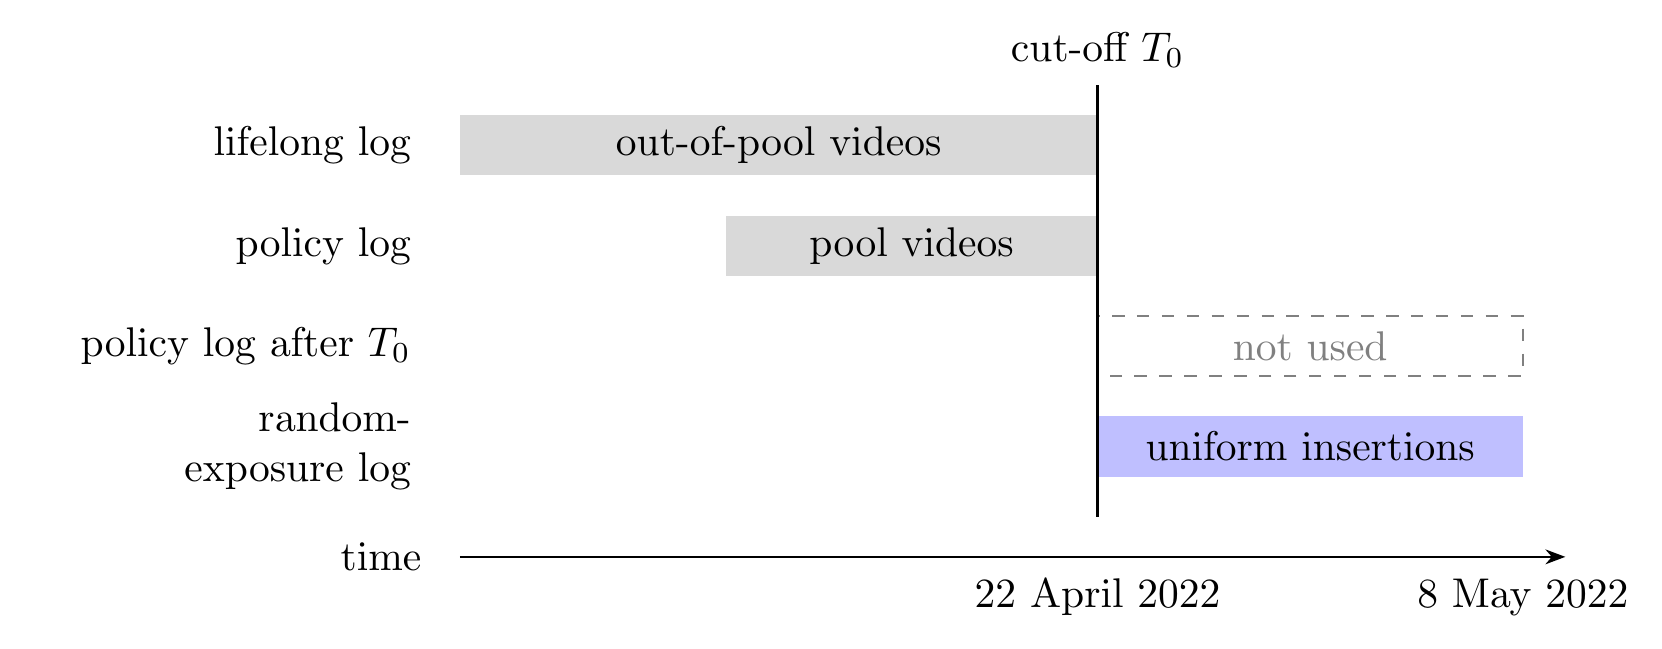
\includegraphics[width=\linewidth]{fig_timeline.png}
\caption{The three logs in time. The lifelong log and the policy log end at the cut-off $T_0$, and the random-exposure log starts
  there. Only the random-exposure log supplies candidates and labels, and only to the validation and test users. The policy log after
  the cut-off is not used. The bars are schematic and not to scale.}
\label{fig:timeline}
\end{figure}

\subsection{LEAF: lifelong exposure-conditional affinities}
\label{sec:method-leaf}

If the viewer clicked cooking videos much more often than her other videos \emph{when they were shown to her}, she probably likes
cooking, and this preference should carry over to the clip. Two details matter. The statistic must be conditional on exposure: the
number of cooking videos she clicked depends on how many the policy chose to show her, whereas the fraction of shown cooking videos she
clicked does not. And a rate from few impressions must be shrunk towards her overall rate.

\paragraph{Statistics} For a user $u$, a key family $k$ and a key value $v$, let $n^k_{uv}$ and $c^k_{uv}$ be the impressions and clicks
in the lifelong log of $u$ on videos whose key in family $k$ is $v$. Let $M_u$ and $C_u^{\mathrm{life}}$ be the total impressions and
clicks of $u$ in that log. The lifelong base rate is the smoothed click rate
\begin{equation}
  r_u=\frac{C_u^{\mathrm{life}}+1}{M_u+2}.
  \label{eq:base-rate}
\end{equation}
The \emph{lift} of value $v$ for $u$ is her click rate on the key, shrunk towards the base rate with $\eta$ pseudo-impressions, minus
the base rate:
\begin{equation}
  \ell^k_{uv}=\frac{c^k_{uv}+\eta\,r_u}{n^k_{uv}+\eta}-r_u .
  \label{eq:lift}
\end{equation}
The lift is positive when she clicks the key more often than her other videos once it is shown, and close to zero when the evidence is
thin. The \emph{familiarity} is
\begin{equation}
  f^k_{uv}=\log\bigl(1+n^k_{uv}\bigr),
  \label{eq:familiarity}
\end{equation}
which records her exposure to the key whatever her response. The two carry different information: a user may have seen a popular author
often and still click that author at her average rate.

\paragraph{Channels} For a candidate $i$, LEAF looks up the statistics of $u$ at the three key values of $i$, which gives the channel vector
\begin{equation}
  z_{ui}=\Bigl(\tilde\ell^{\mathrm{tag}}_{u,v_{\mathrm{tag}}(i)},\ \tilde f^{\mathrm{tag}}_{u,v_{\mathrm{tag}}(i)},\
  \tilde\ell^{\mathrm{author}}_{u,v_{\mathrm{author}}(i)},\ \tilde f^{\mathrm{author}}_{u,v_{\mathrm{author}}(i)},\
  \tilde\ell^{\mathrm{music}}_{u,v_{\mathrm{music}}(i)},\ \tilde f^{\mathrm{music}}_{u,v_{\mathrm{music}}(i)}\Bigr)\in\mathbb R^6,
  \label{eq:channels}
\end{equation}
where each tilde divides a statistic by the standard deviation of its non-zero values over all pairs of users and pool videos, computed
separately for each channel. The channels are not centred, so a channel is zero when the key is absent or $u$ has no lifelong impression
with that value. The channels are computed once from the lifelong log, and scoring a pair is a table lookup.

\subsection{LEAF-LGN: lifelong channels inside a graph recommender}
\label{sec:method-leaflgn}

LightGCN \citep{he2020lightgcn} spreads user and item embeddings over the bipartite graph of clicked pairs $\{(u,i):X_{ui}=1\}$. LEAF-LGN adds
the six channels to its score of a pair:
\begin{equation}
  s^{\mathrm{LEAF}}_{ui}=\langle\bar e_u,\bar e_i\rangle+b_u+b_i+b_0+\beta\,q_i+g^{\top}z_{ui},
  \label{eq:leaflgn}
\end{equation}
where $\bar e_u$ and $\bar e_i$ are the scoring embeddings after two propagation layers, $b_u$, $b_i$ and $b_0$ are user, item and global
biases, $q_i$ is the standardised logarithm of the number of users who clicked $i$ before $T_0$, and $\beta$ and $g\in\mathbb R^6$ are its
weights. All parameters, including $\beta$ and $g$, are learned together, so the model decides how much each lifelong channel is worth
relative to the collaborative signal.

\paragraph{Training} The parameters are fitted with the Bayesian personalised ranking loss \citep{rendle2009bpr},
\begin{equation}
  \mathcal L=-\frac{1}{|B|}\sum_{(u,i,j)\in B}\log\sigma\bigl(s^{\mathrm{LEAF}}_{ui}-s^{\mathrm{LEAF}}_{uj}\bigr)
  +\frac{\rho}{|B|}\sum_{(u,i,j)\in B}\bigl(\|\bar e_u\|^2+\|\bar e_i\|^2+\|\bar e_j\|^2\bigr),
  \label{eq:bpr}
\end{equation}
where $B$ is a mini-batch of triples $(u,i,j)$ in which $i$ is a clicked pair, $\sigma$ is the logistic function and $\rho$ the weight
decay. The negative $j$ is drawn uniformly from the items that $u$ was not shown before $T_0$ (or, when the policy channel is off, did not click).

A policy-log channel, which adds shown but unclicked pairs as weak positives with a weight $w$, was also tried. The LEAF-LGN of the separate search (Section~\ref{sec:protocol-baselines}) selects $w=0$ in four of five splits and
does not lose score without the channel (Section~\ref{sec:res-controls}). The backbone selected for LEAF-LGN+DAX uses $w=0.25$ or
$0.5$ in every split, so the channel is part of that model. Its definition and
its control are in \ref{app:supp}.

\subsection{DAX: detection-adjusted attractiveness}
\label{sec:method-dax}

\paragraph{Idea} A non-click is ambiguous. When the cooking clip is shown and not clicked, either the viewer looked at it and did not find
it attractive, or she never really looked at it, for instance because she was scrolling quickly in a scenario where few videos are watched.
A raw click rate treats every non-click as the first case, and so penalises items that the policy happened to show to inattentive users or
in inattentive scenarios. Occupancy models in ecology \citep{mackenzie2002occupancy} face the same ambiguity: a site can be occupied and still
yield no detection. Click models for web search \citep{richardson2007predicting,craswell2008cascade,chuklin2015clickmodels} write a click as
examination times attraction, with examination depending on rank. DAX applies this separation to a feed. An impression plays the role of a
survey, a click the role of a detection, and the attractiveness of the item the role of presence. A feed slot has no rank, so examination
depends on who is watching and in which scenario.

\paragraph{Generative model} For an impression $r$ of the policy log, DAX introduces latent examination and attraction indicators $E_r$ and
$R_r$:
\begin{equation}
  E_r\sim\mathrm{Bernoulli}\bigl(\theta_{u_r}\kappa_{t_r}\bigr),\qquad
  R_r\sim\mathrm{Bernoulli}\bigl(\alpha_{i_r}\bigr),\qquad
  y_r=E_rR_r ,
  \label{eq:dax-model}
\end{equation}
with $E_r$ and $R_r$ independent. Here $\theta_u\in(0,1]$ is the examination propensity of user $u$, $\kappa_t>0$ is the relative
examination factor of scenario $t$, with $\kappa_1=1$ for the evaluation scenario, and $\alpha_i\in(0,1)$ is the probability that item $i$
is clicked once examined. The quantity of interest is $\alpha_i$. The factors $\theta_u$ and $\kappa_t$ are nuisance parameters that
absorb who saw the item and where.

\paragraph{What a non-click says} Write $\tau_r=\theta_{u_r}\kappa_{t_r}$ for the examination probability of impression $r$. A click implies
$E_r=R_r=1$. After a non-click, Bayes' rule gives
\begin{equation}
  \begin{aligned}
  p_{E,r}&=P(E_r=1\mid y_r=0)=\frac{\tau_r(1-\alpha_{i_r})}{1-\tau_r\alpha_{i_r}},\\
  p_{R,r}&=P(R_r=1\mid y_r=0)=\frac{(1-\tau_r)\,\alpha_{i_r}}{1-\tau_r\alpha_{i_r}} .
  \end{aligned}
  \label{eq:posterior}
\end{equation}
If examination is unlikely, $p_{R,r}\to\alpha_{i_r}$ and the non-click leaves the belief about the item almost unchanged. If examination is
nearly certain, $p_{R,r}\to0$ and the non-click counts fully against the item. A non-click by an attentive user in an attentive scenario is
therefore strong evidence, and one by an inattentive user is weak evidence. An additive model on the logit scale does not have this property
(Section~\ref{sec:res-ablate}).

\paragraph{Priors} Three factors are regularised by pseudo-counts. The attractiveness of item $i$ has a Beta prior with centre $c_{g(i)}$,
the pooled attractiveness of its tag $g(i)$ (items without a tag form one group), and strength $\nu$, so an item with few impressions is pulled
towards its tag. The examination propensity has a Beta prior centred on the user's lifelong rate, $\theta_u\sim\mathrm{Beta}\bigl(\lambda\tilde c_u,\,
\lambda(1-\tilde c_u)\bigr)$ with strength $\lambda$, so a user who clicks rarely on the platform is presumed to examine rarely. The lifelong log
enters DAX only through this one number per user. Each scenario factor receives one pseudo-count in the numerator and one in the denominator of
its update, which pulls the factor of a rarely used scenario towards one.

\paragraph{Estimation} The latent indicators make the likelihood of Equation~\eqref{eq:dax-model} awkward to maximise directly and easy to
handle by EM. The E-step computes $p_{E,r}$ and $p_{R,r}$ of Equation~\eqref{eq:posterior} for every impression, with both equal to one for a
click. The M-step re-estimates the factors in the order $\theta$, $\kappa$, $\alpha$, each time with the most recent values of the others:
\begin{align}
  \theta_u&\leftarrow\frac{\sum_{r:\,u_r=u}p_{E,r}+\lambda\,\tilde c_u}{\sum_{r:\,u_r=u}\kappa_{t_r}+\lambda},
  \label{eq:m-theta}\\
  \kappa_t&\leftarrow\frac{\sum_{r:\,t_r=t}p_{E,r}+1}{\sum_{r:\,t_r=t}\theta_{u_r}+1},\qquad\text{followed by}\quad
  \kappa_t\leftarrow\kappa_t/\kappa_1,
  \label{eq:m-kappa}\\
  \alpha_i&\leftarrow\frac{\sum_{r:\,i_r=i}p_{R,r}+\nu\,c_{g(i)}}{n_i+\nu},
  \label{eq:m-alpha}
\end{align}
where $n_i$ is the number of impressions of item $i$. The attractiveness of an item is its expected number of attractions per impression,
with $\nu$ pseudo-impressions at the tag level added. The ratio-form update for $\theta$ is the exact M-step of the likelihood term when all of a user's impressions come from one
scenario, and the update for $\kappa$ is exact only when examination is constant within a scenario; otherwise both are approximations.
At the fitted values the ratio and exact updates for $\theta$ agree closely, and fitting with exact M-steps does not change the ranking
significantly (\ref{app:em} gives the check and the clamps). The fit runs for a fixed number of iterations from fixed initial values, without a convergence test (\ref{app:em}).

The two prior centres are re-estimated at every iteration. The tag centre is the pooled attraction rate of the tag,
\begin{equation}
  c_g=\frac{\sum_{i:\,g(i)=g}\ \sum_{r:\,i_r=i}p_{R,r}+1}{\sum_{i:\,g(i)=g}n_i+2},
  \label{eq:tag-centre}
\end{equation}
and the lifelong centre rescales the user's lifelong rate to the average examination rate of the policy log,
\begin{equation}
  \tilde c_u=\operatorname{clip}_{[10^{-3},\,1]}\Bigl(\frac{r_u}{\bar r}\cdot\frac{\sum_{r\in\mathcal D}p_{E,r}}{\sum_{r\in\mathcal D}\kappa_{t_r}}\Bigr),
  \label{eq:life-centre}
\end{equation}
where $\bar r$ is the mean of $r_u$ over users. The only user-specific factor is $r_u/\bar r$, and a user without lifelong history receives the
mean centre.

\paragraph{Output} After the fixed number of iterations, DAX returns the attractiveness of every pool item and discards the examination
factors. The item score passed on is the standardised logit
\begin{equation}
  \zeta_i=\frac{\operatorname{logit}\alpha_i-\mu_\alpha}{\sigma_\alpha},
  \label{eq:zeta}
\end{equation}
where $\mu_\alpha$ and $\sigma_\alpha$ are the mean and standard deviation of $\operatorname{logit}\alpha$ over $\mathcal I$. The score
$\zeta_{ui}$ of a candidate in Section~\ref{sec:method-combine} equals $\zeta_i$, unless the user-group refinement is used, in which case
it is the score of the user's group (\ref{app:em}). In the running
example, if most of the clip's non-clicks came from users with a low lifelong click rate or from a scenario with a small factor $\kappa_t$, DAX
attributes them mostly to missed examination, and the clip receives a higher attractiveness than its raw click rate suggests.

\paragraph{Optional refinements} The DAX module has two refinements, chosen on validation users. The first replaces the tag centre, after a fixed number of initial iterations, by a ridge regression on content codes in the spirit of small-area estimation \citep{fay1979smallarea}:
\begin{equation}
  c_i=\sigma\bigl(\mu_0+\mathbf x_i^{\top}\boldsymbol\beta\bigr),\qquad
  \boldsymbol\beta=\bigl(\mathbf X^{\top}W\mathbf X+\xi\,I\bigr)^{-1}\mathbf X^{\top}W\bigl(\mathbf y-\mu_0\mathbf 1\bigr),
  \label{eq:content-centre}
\end{equation}
where $\mathbf y$ is the vector of $\operatorname{logit}\alpha_i$ over the pool, $\mathbf X$ stacks the one-hot content codes $\mathbf x_i$ of the
pool videos, $W=\operatorname{diag}(w_i)$ with $w_i=\sqrt{n_i+1}$, $\mu_0$ is the weighted mean of $\mathbf y$, and $\xi$ is a fixed ridge penalty. The validation selection chose this centre in one of the
five splits.
The second refinement estimates the attractiveness separately for six groups of users, defined by the lifelong base rate. It was on in
all five splits of the reported model, but it is optional and adds no measurable gain (Section~\ref{sec:res-exam}),
and its description is in \ref{app:em}. Each lifelong, tag and scenario component can be turned off in the ablations
(Section~\ref{sec:res-ablate}).

\subsection{Combining LEAF-LGN and DAX}
\label{sec:method-combine}

DAX produces one number per item and does not depend on the backbone, so it is added after the backbone has been trained. For a user
$u$ with candidate list $C_u$, the final score of a candidate $i\in C_u$ is
\begin{equation}
  s_{ui}=\operatorname{std}_{C_u}\bigl(s^{\mathrm{LEAF}}_{ui}\bigr)+\gamma\,\operatorname{std}_{C_u}\bigl(\zeta_{ui}\bigr),
  \label{eq:combine}
\end{equation}
where $\operatorname{std}_{C_u}$ subtracts the mean over the candidate list and divides by its standard deviation, so that both terms are on
the same scale for every user, and $\gamma\ge0$ is the weight of DAX. With $\gamma=0$ the score is that of the backbone.

The weight $\gamma$, the DAX settings and the training epoch are selected together on validation users. At every epoch, every DAX configuration
and every value of $\gamma$ are scored, and the best validation combination is kept. Because $\gamma=0$ is among the candidates, the combination
cannot be worse than its backbone on validation users, and the weight is a hyperparameter rather than a learned parameter. The same rule defines a
DAX variant of every other backbone in our experiments. Algorithms~\ref{alg:dax} and~\ref{alg:leaflgn} in \ref{app:supp} summarise the fit and the selection.

\subsection{What the attractiveness measures}
\label{sec:method-identify}

The probability of a click depends on the parameters only through $\theta_u\kappa_t\alpha_i$. For any constant $a>0$, the transformation
$(\theta,\alpha)\mapsto(a\theta,\alpha/a)$ leaves the likelihood unchanged while all values stay in $[0,1]$. The normalisation $\kappa_1=1$ fixes
the scale of the scenario factors, but one global scale shared by $\theta$ and $\alpha$ remains, and the priors and bounds fix it in practice.
The ordering of items by $\alpha_i$ is therefore meaningful, but its values are not click probabilities. The logit in Equation~\eqref{eq:zeta} is
not scale-invariant, which is why $\nu$ and $\lambda$ are selected on validation users. The factors $\theta_u$ and $\kappa_t$ should not be read as
user traits or scenario properties; their role is to explain away non-clicks that carry little information about the item. Finally, $\alpha_i$ is
model-based under the independence of examination and attraction in Equation~\eqref{eq:dax-model}. We do not claim that it is an unbiased or
causally identified measure of item quality. We test only whether it improves the ranking of randomly inserted items.

\section{Experimental protocol}
\label{sec:protocol}

This section defines the temporal split, the data, the selection rule, the significance rule and the baselines. Leakage checks,
search grids and the secondary controls are in \ref{app:supp} and~\ref{app:grids}.

\subsection{Temporal protocol}
\label{sec:protocol-temporal}

The random-exposure period starts on 22 April 2022 at 00:00 UTC+8, and this instant is the cut-off $T_0$. Every quantity used for training
or selection is computed before $T_0$. This includes the in-pool click matrix and the standard log used by the backbones, the lifelong
tables, the DAX fit, the popularity offset and the negative sampler. A pair shown before $T_0$ is excluded from its user's candidate list.
The cut-off matters because the policy keeps logging after a random impression, so a log that extends past $T_0$ can contain the user's
later responses to the inserted video. The random-exposure data serve two purposes only. The candidate lists and labels of validation users
select the configuration, and those of test users measure the score. No model reads them for training, since a method trained on uniform
labels would be measured on its own training target.

\subsection{Data, users and splits}
\label{sec:protocol-data}

The primary dataset is KuaiRand-27K \citep{gao2022kuairand}. Its users are all users that appear in both the standard log and the random log,
and its pool is the set of random-log videos. Table~\ref{tab:data} gives the sizes. The secondary dataset, KuaiRand-1K, comes from the same
release, with 1,000 users of whom 993 appear in both logs. Its identifiers are those of the 27K release, so it is a replication at smaller
scale rather than an independent sample (\ref{app:counts}). Coat \citep{schnabel2016} and Yahoo! R3 \citep{marlin2009collaborative} have no impressions that were shown and left unrated, and no history on other items. KuaiRec \citep{gao2022kuairec} has no scenario field and no history outside its matrix, and the Open Bandit Dataset \citep{saito2021obd} has no persistent user identifiers.

\begin{table}[tbp]
\centering
\caption{Sizes of the two KuaiRand settings under the temporal protocol.}
\label{tab:data}
\footnotesize
\begin{tabular}{p{0.5\textwidth}p{0.22\textwidth}p{0.22\textwidth}}
\toprule
Quantity & KuaiRand-27K & KuaiRand-1K \\
\midrule
Users in both logs (dataset users) & 27,077 & 993 \\
Pool items & 7,583 & 7,388 \\
Pre-cut training clicks & 523,176 & 18,873 \\
Pre-cut training impressions & 1,141,300 & 40,738 \\
Users with a pre-cut lifelong history & 26,904 (LEAF statistics); 26,723 (sequence models) & 983 (LEAF statistics); 977 (sequence models) \\
Out-of-pool impressions before $T_0$ & 135,219,168 & 5,016,818 \\
Random-exposure rows & 1,186,059 & 42,944 \\
Test users (candidate lists) & 27,077 & 993 \\
Test users with a click, pooled & 22,612 & 842 \\
Test users with a click, per split & 15,809 to 15,913 & 579 to 591 \\
Candidates per user (temporal), mean (median) & 43.6 (22) & 43.2 (22) \\
\bottomrule
\end{tabular}
\end{table}

Each split partitions the test users by user, not by impression. Split $s\in\{0,\dots,4\}$ takes a random permutation of the users with seed
$s$, and the first 30\% of the permuted users (rounded to the nearest integer) form the validation set. For KuaiRand-27K this is 8,123
validation and 18,954 test users in each split. The backbones are trained once for each hyperparameter setting on the whole pre-cut log, and
every split reads the same training trajectory. The splits change only which users select the epoch, the configuration and $\gamma$, and which
users are scored. This is why a split-level test is reported next to the per-user test.

\subsection{Ranking metrics}
\label{sec:protocol-metrics}

Six ranking metrics are reported for every method: nDCG@5, nDCG@10, nDCG@20, Recall@10, Recall@20 and the mean reciprocal rank (MRR). Each is
computed for each test user on that user's candidate list, in which the clicked candidates are the relevant items. Users without a clicked
candidate are excluded, since nDCG and recall are then undefined. nDCG@$k$ discounts the candidate at rank $r$ by $1/\log_2(r+1)$ and divides the
discounted gain of the top $k$ by the largest gain attainable with the same number of relevant items in $k$ positions. Recall@$k$ is the share of
the user's clicked candidates that appear in the top $k$. MRR is the reciprocal of the rank of the first clicked candidate. The split value of each
metric is the mean over the users of that split, and the table entries are means over the five splits.

\subsection{Selection and search budgets}
\label{sec:protocol-selection}

For each split the selected configuration is the one with the largest validation nDCG@10, and no other metric enters the choice of any
configuration; the other five metrics are read at the configuration so selected. The test labels are read only for the configuration
that is best on validation so far, and no test label influences the choice of any configuration. The configurations searched are the backbone
trainings times the DAX configurations times the values of $\gamma$; epochs are selected inside each training and counted as evaluations, not
as configurations. LEAF-LGN+DAX searches $12\times32\times10=3{,}840$ configurations, PW-LightGCN+DAX $10\times32\times10=3{,}200$, DIN+DAX 1,280,
and PW-LightGCN itself 20. The budgets are not matched. The fair comparator for the DAX module is PW-LightGCN with the same module
(Section~\ref{sec:res-fair}), and every count and mean is listed in \ref{app:counts}.

\subsection{Statistics and the significance rule}
\label{sec:protocol-stats}

There is one significance rule. A comparison is called significant only when its Holm-adjusted split-level p value, for the test named in the
table, is below 0.05, where the adjustment runs over the family named in that table. An adjusted value between 0.04 and 0.05 is called
significant but narrow, and is not rounded in either direction. Comparisons outside a stated family are reported unadjusted and are not called
significant.

The split-level test is the Nadeau-Bengio corrected resampled t test \citep{nadeau2003} applied to the five split means $\bar d$ of the split
differences $d_s$. With $J=5$ splits the variance of the mean is estimated as
$\widehat{\mathrm{Var}}=s_d^2\bigl(\tfrac1J+\tfrac{n_{\mathrm{test}}}{n_{\mathrm{val}}}\bigr)=s_d^2\bigl(\tfrac15+\tfrac73\bigr)$, where $s_d^2$ is the
sample variance of the split differences. The statistic $t=\bar d/\sqrt{\widehat{\mathrm{Var}}}$ is compared with a t distribution with four
degrees of freedom. The correction assumes resampled training sets, and here all splits share one training run, so the split-level values are
approximate. With four degrees of freedom, a two-sided test at 0.05 needs a ratio of mean to standard deviation of the split differences of at
least $t_{0.975,4}\sqrt{1/5+7/3}\approx4.42$. With five splits the test has low power.

The per-user test is secondary. For two methods $A$ and $B$, the difference of a user is the mean, over the splits in which the user is scored,
of the difference of the two nDCG@10 values. Tables report the mean of these user differences, multiplied by $10^{3}$, with a 95\% half-width from
the two-sided t interval over users. The per-user p value is that of a two-sided one-sample t test. Users appear in several splits and share one
training run, so this test treats users as independent when they are not, and it is reported only in \ref{app:sens}.

Two quantities appear in the tables. The \emph{mean} is the mean of the five split means. The \emph{difference} is the mean over the pooled test
users of each user's paired difference. These weight users and splits differently, so a difference need not equal the difference of the two means
shown.

Holm's step-down procedure \citep{holm1979} adjusts each family. The families are as follows.
\begin{itemize}
\item Main family, thirteen comparisons, each against LEAF-LGN+DAX: PW-LightGCN, PW-LightGCN+DAX, LEAF-LGN, r-AdjNorm, LightGCN, DIN, DIN+DAX,
  SIM, SIM+DAX, NAVIP, IPS-MF, DR-JL and MRDR.
\item Sensitivity family, fifteen comparisons: the main family plus EASE and EASE+DAX (\ref{app:sens}).
\item The six DAX increments of Table~\ref{tab:backbone}.
\item The four matched-capacity comparisons of Table~\ref{tab:deep}, the four comparisons of the examination control of
  Table~\ref{tab:exam}, and the seed comparisons of Tables~\ref{tab:seeds-din} and~\ref{tab:seeds-pw}, each adjusted over the two seeds of its comparator.
\item Seven gains and six full-minus-variant differences of the ablations (Section~\ref{sec:res-ablate}).
\item Three LEAF-LGN controls (Section~\ref{sec:res-controls}), and three comparisons on KuaiRand-1K.
\end{itemize}
The primary criterion was written down before the main experiment, when the primary family had five members: LEAF-LGN+DAX against PW-LightGCN,
PW-LightGCN+DAX, the LEAF-LGN backbone, r-AdjNorm and LightGCN. It requires a margin of at least $15\times10^{-3}$ over PW-LightGCN and both
adjusted values below 0.05. Later the main family was extended by DIN, SIM and the four published estimators, which is why the adjusted value
against PW-LightGCN is 0.023 in the family of five and 0.0456 in the family of thirteen. The family of thirteen is the test used in the main
text, and both values are reported in Section~\ref{sec:res-main}.

\subsection{Baselines}
\label{sec:protocol-baselines}

The baselines are LightGCN, r-AdjNorm (LightGCN with a normalisation exponent in $\{0.3,0.7\}$), EASE, PW-LightGCN, LEAF-LGN without DAX, two
lifelong deep models and four published debiased estimators. PW-LightGCN is our own propensity-weighted LightGCN, described in full in
\ref{app:qp}; it has not been published, and it searches 20 configurations. DIN \citep{zhou2018din} attends over the last 200 pre-cut
events of the user on videos outside the pool. SIM-hard \citep{pi2020sim} keeps the 50 most recent of these events that share the tag or author
of the candidate, and attends over them. Both use identifier embeddings and the BPR loss, and both are searched over four trainings, of dimension
16, at most 12 epochs and patience 2. The published estimators are NAVIP \citep{kim2022navip}, IPS-MF \citep{schnabel2016}, DR-JL \citep{wang2019drjl}
and MRDR \citep{guo2021mrdr}. All four use a propensity estimated from item popularity, dimension 64, at most 40 epochs and four configurations.
Their search is much narrower than that of LEAF-LGN+DAX, and their values are conditional on it. Matched-capacity runs of the same two
lifelong models, with dimension 64, are described in Section~\ref{sec:res-deep}. TWIN \citep{chang2023twin} is not used as a
baseline. Every backbone with DAX gets the same DAX module and the same $\gamma$ grid as LEAF-LGN. \ref{app:grids} gives the grids.

Several values of LightGCN and LEAF-LGN appear, each from its own search. The main table uses the four-configuration LightGCN (0.4576). The DAX increment on
LightGCN is measured against a LightGCN trained in the same run as its DAX variant (0.4597), because the base and the variant must come from the
same search. The LEAF-LGN of the main table (0.4736) is selected from twelve trainings over the learning rate, the weight decay and the policy
weight $w\in\{0,0.25,0.5\}$. That grid includes $w=0$, and the selected $w$ is zero in every split, whereas the LEAF-LGN+DAX backbone selects
$w=0.25$ or $0.5$ in every split. The DAX increment on LEAF-LGN therefore also contains the difference between these two backbone trainings. A
second search, run separately over the backbone alone with 197 configurations (the separate search), gives 0.4728 for LEAF-LGN.

\subsection{Ablation design}
\label{sec:protocol-ablation}

The ablations use a reduced search, chosen to keep the cost manageable. Each variant is selected per split in the same way as full DAX, with the
two backbone trainings and the epoch window of three around the epoch chosen in the main experiment, and five values of $\gamma$,
$\{0.1,0.25,0.5,0.7,1.0\}$. The variants are the three DAX switches (without scenario factors, without lifelong prior, without tag prior; 16
configurations each), the additive logit model with user and scenario effects (32 configurations), and the two permutations of attractiveness,
within tags and across all items, each with three permutation seeds. The ablation base is its own LEAF-LGN, selected inside the restricted window.
It is lower than the main LEAF-LGN, so gains against it are not the main-table increment, and comparisons between variants use the full-minus-variant
differences, which do not use the base. Full DAX in the ablation search selects the same configurations as in the main experiment on all five
splits and reproduces its test values. The examination control of Section~\ref{sec:res-exam} uses the same search with the
examination factors fixed to one.

\subsection{Kinds of number}
\label{sec:protocol-kinds}

Main results are selected on validation users and measured on test users. Diagnostic quantities use random-exposure labels to locate headroom;
they are never used to select or train a method, and they are marked as diagnostic. Preliminary analyses on fixed backbone scores appear only in
\ref{app:controls}.

\section{Results}
\label{sec:results}

Differences are means of per-user nDCG@10 differences, multiplied by $10^{3}$, with the 95\% half-width in brackets. Each table states
the Holm family of its adjusted values. Each subsection gives the question and the answer first.

\subsection{Headroom diagnosis}
\label{sec:res-headroom}

This subsection is a diagnostic. It uses random-exposure labels, including those of the test users, and it is never used to select or train a
method. We ask how much accuracy the item level could add. On the 22,661 users with a click in some candidate list, a leave-one-user-out item
oracle, which scores each candidate by the uniform click rate of the item among the other users, reaches nDCG@10 0.5068. LEAF-LGN, with the
configuration selected on the first split, reaches 0.4735, a gap of $33.31\times10^{-3}$. The method, LEAF-LGN+DAX, reaches 0.4854 as a mean over
five splits, which closes about 36\% of the gap. The two sides use slightly different user sets, so this share is approximate. The lifelong user
channels alone gain $10.65$ to $11.46\times10^{-3}$ (Section~\ref{sec:res-controls}), so the remaining headroom lies at the user level as well as at
the item level, and this diagnostic does not separate the two.

\subsection{Main comparison}
\label{sec:res-main}

We ask whether LEAF-LGN+DAX is more accurate than each baseline. The answer is yes on the per-user test against all thirteen comparators, and on the
split-level test against all thirteen after Holm correction. Two of these margins are significant but narrow (adjusted split-level value 0.0456). Table~\ref{tab:main} gives the paired
comparisons, and Figure~\ref{fig:forest} shows that the sign of each difference is positive in every split.

The closest comparator is DIN+DAX (0.4796), with a difference of $+5.73$ [1.64] and an adjusted split-level p value of 0.0456. The margin is consistent in sign and significant in each re-run, under matched capacity (Section~\ref{sec:res-deep}) and under two further training seeds (Section~\ref{sec:res-seeds}): $+9.67$ under matched capacity and $+9.99$ and $+6.76$ under the two seeds, against $+5.73$ in the main comparison. The second narrow
comparison is PW-LightGCN (0.4634), with a difference of $+22.32$ [1.83] and the same adjusted value of 0.0456 in the family of thirteen. Under two further training seeds the margin is unchanged, at about $22\times10^{-3}$, and the split-level p value is below 0.001 (Section~\ref{sec:res-seeds}). The
pre-specified criterion of the primary family of five, a margin of at least $15\times10^{-3}$ with both adjusted values below 0.05, is met, with an
adjusted split-level value of 0.023 in that family. The four published estimators are far below LEAF-LGN+DAX. NAVIP (0.4579) is close to LightGCN
(0.4576), with a difference of $+27.80$ [1.91]. IPS-MF (0.3765), DR-JL (0.3823) and MRDR (0.3826) each use four configurations, and their values are
conditional on that budget. Adding EASE and EASE+DAX to the family (\ref{app:sens}) leaves every conclusion at the 0.05 level unchanged.

\begin{table}[tbp]
\centering
\footnotesize
\caption{Main results on KuaiRand-27K: LEAF-LGN+DAX against every comparator of the main family, with the paired per-user difference and the split-level (Nadeau-Bengio) test.}
\label{tab:main}
\begin{adjustbox}{max width=\linewidth}
\begin{tabular}{lrccc}
\toprule
Comparator & Mean & Diff.\ [95\% hw] & NB $p$ & NB $p_{\mathrm{Holm}}$ \\
\midrule
LEAF-LGN+DAX (reference) & 0.4854 & n/a & n/a & n/a \\
\midrule
\multicolumn{5}{l}{Holm family: LEAF-LGN+DAX minus each comparator} \\
PW-LightGCN & 0.4634 & +22.32 [1.83] & 0.023 & $4.56\times10^{-2}$ \\
PW-LightGCN+DAX & 0.4733 & +12.04 [1.63] & 0.006 & $2.23\times10^{-2}$ \\
LEAF-LGN & 0.4736 & +11.96 [1.47] & 0.001 & $8.22\times10^{-3}$ \\
r-AdjNorm & 0.4620 & +23.79 [1.96] & $<0.001$ & $3.52\times10^{-4}$ \\
LightGCN & 0.4576 & +28.15 [1.86] & 0.008 & $2.44\times10^{-2}$ \\
DIN & 0.4675 & +18.26 [1.97] & 0.001 & $7.73\times10^{-3}$ \\
DIN+DAX & 0.4796 & +5.73 [1.64] & 0.043 & $4.56\times10^{-2}$ \\
SIM & 0.4590 & +26.44 [2.01] & $<0.001$ & $2.85\times10^{-4}$ \\
SIM+DAX & 0.4706 & +14.72 [1.77] & $<0.001$ & $6.13\times10^{-3}$ \\
NAVIP & 0.4579 & +27.80 [1.91] & 0.003 & $1.26\times10^{-2}$ \\
IPS-MF & 0.3765 & +108.09 [3.09] & $<0.001$ & $2.80\times10^{-6}$ \\
DR-JL & 0.3823 & +102.17 [3.05] & $<0.001$ & $1.17\times10^{-5}$ \\
MRDR & 0.3826 & +102.00 [3.01] & $<0.001$ & $5.14\times10^{-6}$ \\
\midrule
\multicolumn{5}{l}{Outside the main family (split-level values not adjusted)} \\
EASE & 0.4507 & +35.24 [2.24] & $<0.001$ & n/a \\
EASE+DAX & 0.4623 & +23.26 [1.98] & $<0.001$ & n/a \\
\bottomrule
\end{tabular}
\end{adjustbox}
\par\smallskip
\begin{minipage}{\linewidth}\raggedright\footnotesize Mean: the mean of the five split means. Diff.: the mean over the pooled test users of each user's paired difference (a user's difference is averaged over the splits in which the user is scored). The two are computed over different weightings, so a difference need not equal the difference of the two means shown. Diff. is in units of $10^{-3}$, with the 95\% half-width of the t interval over the n = 22,612 pooled test users. NB: Nadeau-Bengio corrected resampled t test over the five split means. NB $p_{\mathrm{Holm}}$: Holm adjustment over the 13 comparators of the main family. NAVIP, IPS-MF, DR-JL and MRDR are published debiased estimators, each tuned over four configurations. LightGCN is the four-configuration LightGCN baseline (a LightGCN trained in the same run as its DAX variant appears in Table~\ref{tab:backbone}). SIM denotes SIM-hard. Per-user p values are in Table~\ref{tab:sens}.\end{minipage}
\end{table}


\begin{figure}[tbp]
\centering
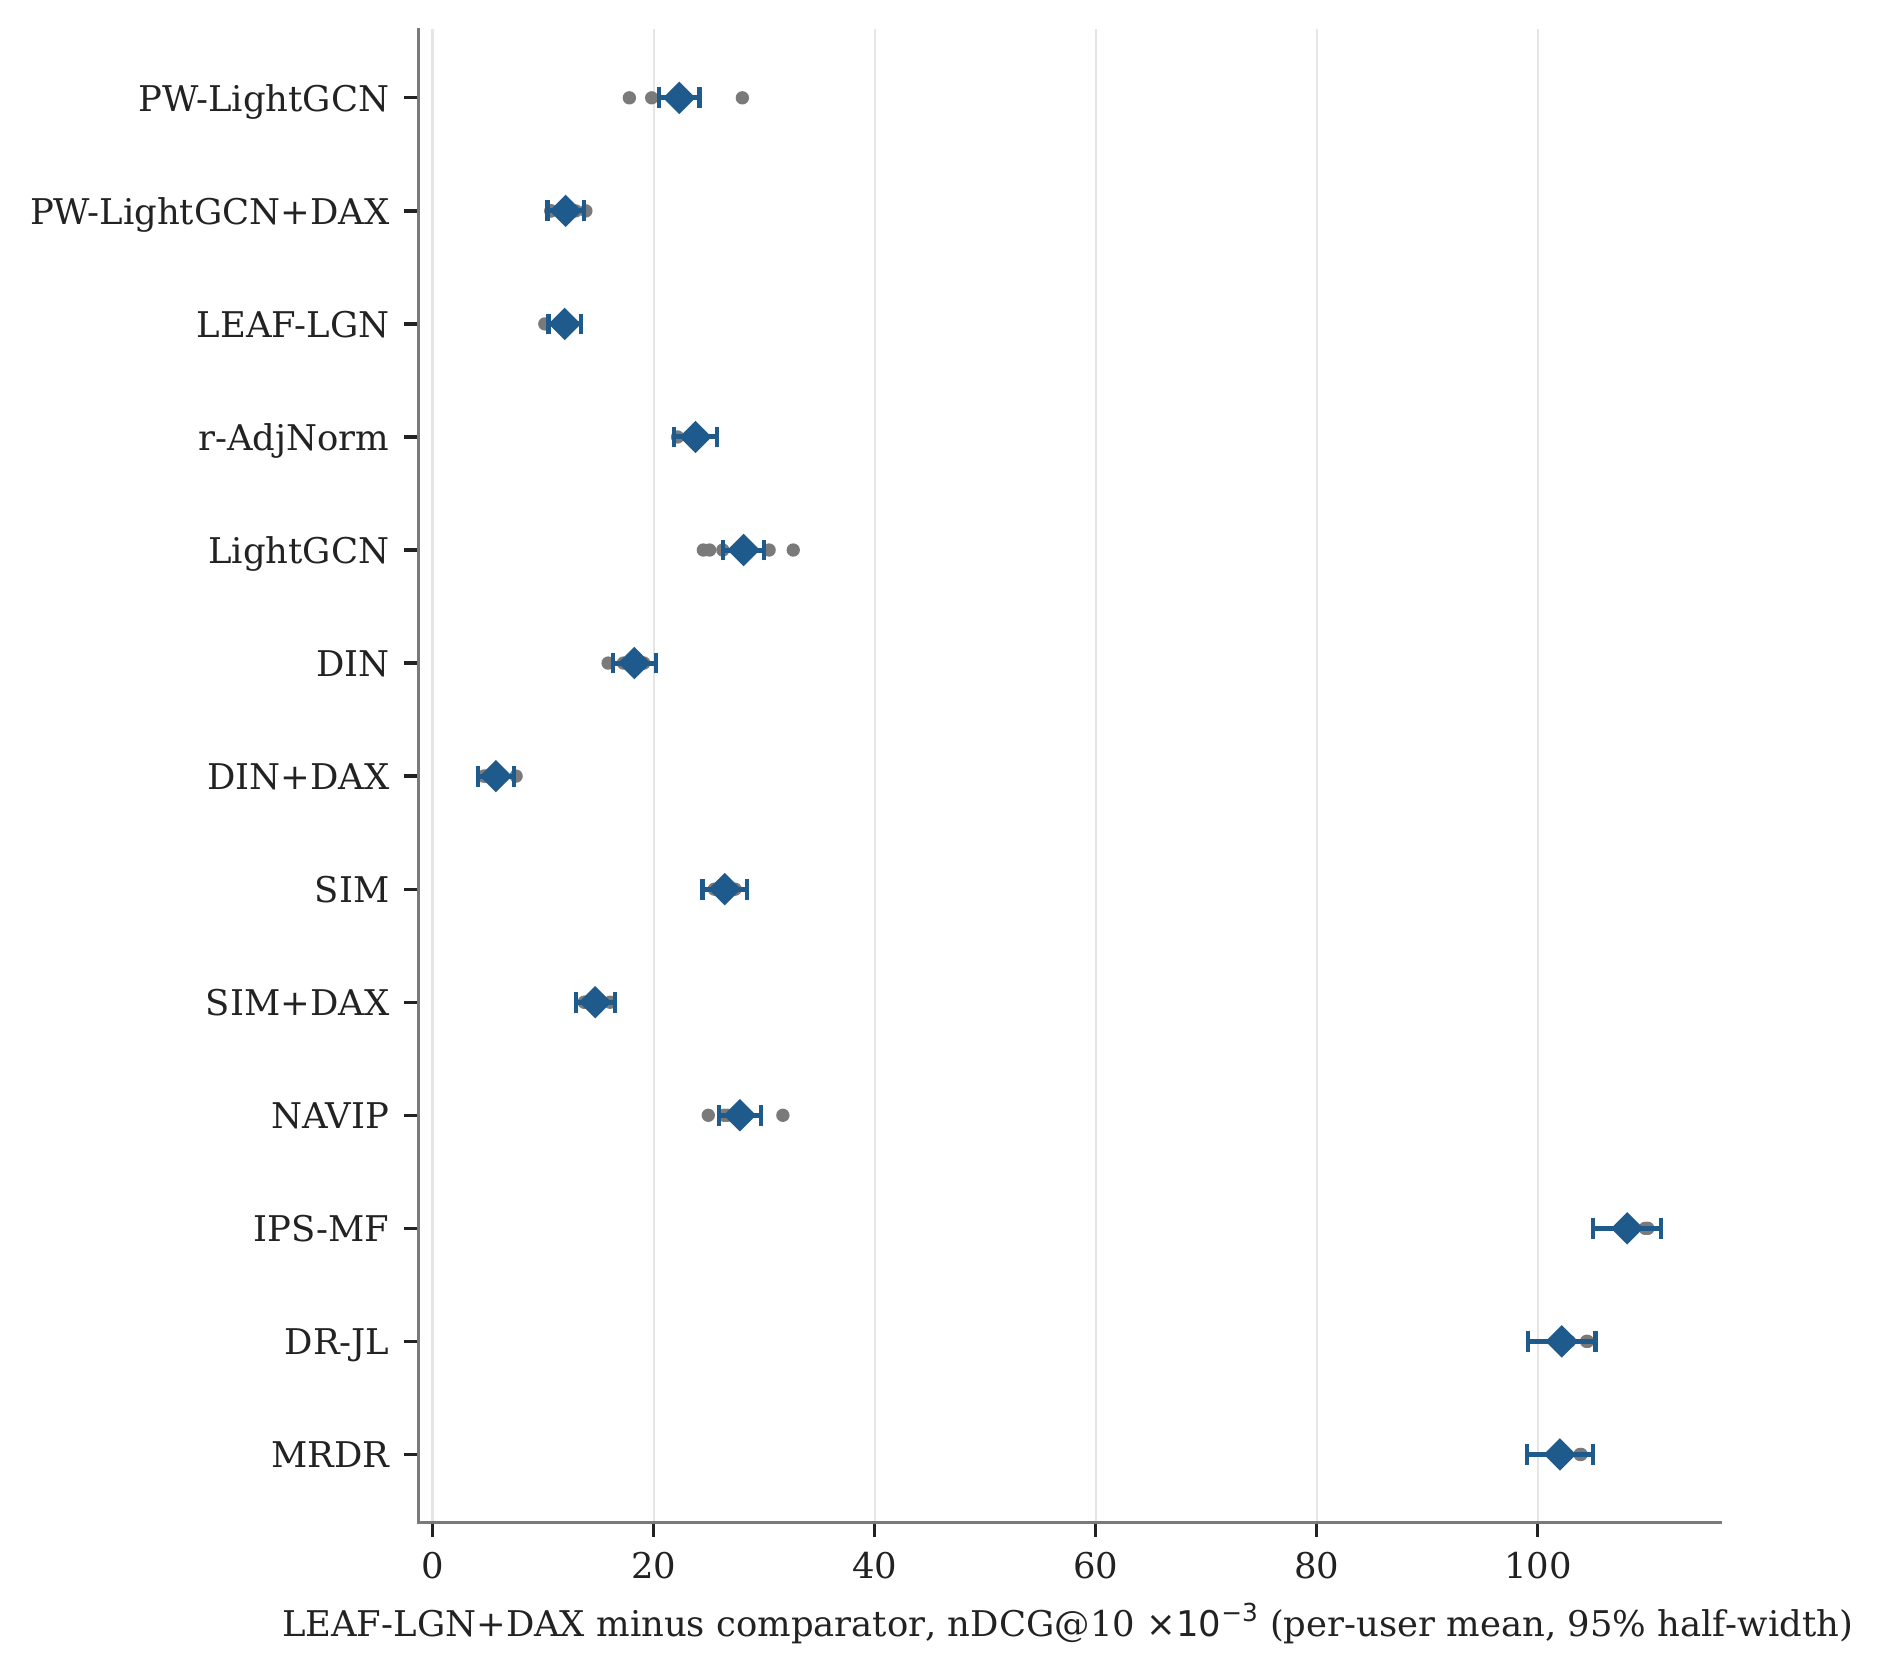
\includegraphics[width=0.85\linewidth]{fig_forest.png}
\caption{Paired differences of LEAF-LGN+DAX against each of the thirteen comparators of the main family, in units of $10^{-3}$ nDCG@10.
  Each grey dot is the difference in one of the five splits. The diamond is the pooled per-user mean difference, with its 95\%
  half-width. Positive values favour LEAF-LGN+DAX. SIM denotes SIM-hard, and PW-LightGCN is the propensity-weighted LightGCN.}
\label{fig:forest}
\end{figure}

\subsection{Other ranking metrics}
\label{sec:res-metrics}

We ask whether the ordering of the methods depends on the metric. The leader does not change: LEAF-LGN+DAX is highest on all six metrics, and
DIN+DAX is second on all six. Table~\ref{tab:metrics} in \ref{app:metrics} gives the six means and marks each cell whose split-level difference from LEAF-LGN+DAX
is not significant at 0.05. Without adjustment for the number of metrics, every other difference is significant at split level. Against DIN+DAX only nDCG@10
is significant, and narrowly (p 0.043); the other five metrics give p values between 0.079 and 0.192. Against PW-LightGCN+DAX the MRR difference is
not significant (p 0.070). Below the leading two, the order shifts with the metric: under the two recall metrics LEAF-LGN and DIN rank above the DAX
variants of PW-LightGCN and LightGCN, and under the other four metrics they rank below them.

\subsection{Comparison with the same DAX module}
\label{sec:res-fair}

We ask whether the advantage comes from the DAX module or from the search budget. The answer is that the module accounts for part of it: against PW-LightGCN with the same module (Table~\ref{tab:fair}), LEAF-LGN+DAX is higher by $+12.04$ [1.63], with an adjusted split-level value of 0.0223. PW-LightGCN gains $+10.28$ [1.37]
from DAX on its own backbone, but the split-level p value is 0.105, so that increment is not established at split level. The LEAF-LGN backbone with its
separate search is $+9.63$ [1.60] above PW-LightGCN, with an unadjusted split-level p value of 0.063. The LEAF backbone alone is therefore not established
as an improvement over PW-LightGCN at split level, whereas the combination is. PW-LightGCN with DAX searches only the backbones selected without DAX,
which is conservative for the method.

\begin{table}[tbp]
\centering
\footnotesize
\caption{Fair-baseline reading: the DAX increments, and LEAF-LGN without DAX against the PW-LightGCN, with the configurations searched by each method (first and second method in the second column).}
\label{tab:fair}
\begin{adjustbox}{max width=\linewidth}
\begin{tabular}{lcccc}
\toprule
Comparison & Configurations & Diff.\ [95\% hw] & NB $p$ & NB $p_{\mathrm{Holm}}$ \\
\midrule
LEAF-LGN+DAX minus PW-LightGCN+DAX (fair baseline) & 3,840 / 3,200 & +12.04 [1.63] & 0.006 & $2.23\times10^{-2}$ \\
PW-LightGCN+DAX minus PW-LightGCN (DAX on the PW-LightGCN backbone) & 3,200 / 20 & +10.28 [1.37] & 0.105 & n/a \\
LEAF-LGN+DAX minus LEAF-LGN (DAX on the LEAF backbone) & 3,840 / 12 & +11.96 [1.47] & 0.001 & $8.22\times10^{-3}$ \\
LEAF-LGN (separate search) minus PW-LightGCN & 197 / 20 & +9.63 [1.60] & 0.063 & n/a \\
\bottomrule
\end{tabular}
\end{adjustbox}
\par\smallskip
\begin{minipage}{\linewidth}\raggedright\footnotesize Diff. and NB $p$ are defined as in Table~\ref{tab:main}. NB $p_{\mathrm{Holm}}$ is given for the two comparisons of the main family; the other two values are not adjusted. The PW-LightGCN with DAX searches only the PW-LightGCN backbone configurations selected without DAX.\end{minipage}
\end{table}


\subsection{DAX on six backbones}
\label{sec:res-backbone}

We ask whether DAX helps backbones other than LEAF-LGN. Table~\ref{tab:backbone} gives the six increments. The answer is that the per-user increment is positive on all six, and that the split-level
increment is significant on five after Holm correction over the six. PW-LightGCN is the exception, with a split-level p value of 0.105. The LightGCN
increment depends on its base. Against the LightGCN of the same run it is $+11.60$ [1.51] (adjusted 0.005). Against the four-configuration LightGCN of the
main table it is $+13.73$ [1.46], with an unadjusted split-level p value of 0.091, which is not significant after adjustment over the six (0.182). Each
row uses its own base, so the increments are not comparable with the main difference of LEAF-LGN+DAX.

\begin{table}[tbp]
\centering
\footnotesize
\caption{DAX on six backbones on KuaiRand-27K: nDCG@10 without and with the DAX module, the paired per-user difference in units of $10^{-3}$ with its 95\% half-width, and the split-level Nadeau-Bengio test. SIM denotes SIM-hard.}
\label{tab:backbone}
\begin{adjustbox}{max width=\linewidth}
\begin{tabular}{lrrccc}
\toprule
Backbone & Without DAX & With DAX & Diff.\ [95\% hw] & NB $p$ & NB $p_{\mathrm{Holm}}$ \\
\midrule
EASE & 0.4507 & 0.4623 & +11.98 [1.64] & $<0.001$ & $<0.001$ \\
LightGCN (same-run base) & 0.4597 & 0.4709 & +11.60 [1.51] & $<0.001$ & 0.005 \\
PW-LightGCN & 0.4634 & 0.4733 & +10.28 [1.37] & 0.105 & 0.105 \\
LEAF-LGN & 0.4736 & 0.4854 & +11.96 [1.47] & 0.001 & 0.005 \\
DIN & 0.4675 & 0.4796 & +12.53 [1.41] & 0.011 & 0.025 \\
SIM & 0.4590 & 0.4706 & +11.72 [1.46] & 0.008 & 0.025 \\
\bottomrule
\end{tabular}
\end{adjustbox}
\par\smallskip
\begin{minipage}{\linewidth}\raggedright\footnotesize Mean: the mean of the five split means. Diff.: the mean over the pooled test users of each user's paired difference (a user's difference is averaged over the splits in which the user is scored). The two are computed over different weightings, so a difference need not equal the difference of the two means shown. NB $p$: split-level Nadeau-Bengio test of each increment. NB $p_{\mathrm{Holm}}$: Holm adjustment over the six increments of this table, the family used for the split-level statements of Section~\ref{sec:res-backbone}. The LightGCN row uses the LightGCN of the same experiment as its DAX variant (three base configurations; 960 with DAX). Against the four-configuration LightGCN of Table~\ref{tab:main} the increment is +13.73 [1.46] (NB $p$ 0.091; NB $p_{\mathrm{Holm}}$ 0.182 over the six increments with that base).\end{minipage}
\end{table}


\subsection{Ablations of DAX}
\label{sec:res-ablate}

We ask which parts of DAX matter. The answer is that the full DAX gain over its base is significant (adjusted 0.037), that permuting attractiveness across items reduces it to zero per user, and that permuting within tags keeps 41.6\% of it. Across items the gain is $-0.27$ [0.36], which is not distinguishable from zero (adjusted
0.754). Within tags it is $+6.28$ [1.10] (adjusted 0.007). Over the three permutation seeds the across-item gains lie between $-0.44$ and $-0.16$, and the
within-tag gains between $+5.66$ and $+6.84$ (Table~\ref{tab:ablate}, lower block). Each removal of a DAX component lowers the per-user score. Removing the scenario factors lowers the score by $1.51$ [0.79], removing the lifelong prior by $1.78$ [0.61], removing the tag prior by $3.41$ [0.99], and the additive model by $6.09$ [0.96]. None of these six full-minus-variant differences is significant at split level: the smallest adjusted value over the six is 0.088.
The per-user evidence therefore favours full DAX over each variant, but the split-level evidence does not separate the three switches or the additive
model from full DAX.

\begin{table}[tbp]
\centering
\footnotesize
\caption{DAX ablations on KuaiRand-27K: gain over the LEAF-LGN base of the ablation experiment, the difference of full DAX to each variant, and the permutation controls.}
\label{tab:ablate}
\begin{adjustbox}{max width=\linewidth}
\begin{tabular}{lrrrcrcr}
\toprule
Variant & Configs & Mean & Gain [95\% hw] & NB $p_{\mathrm{Holm}}$ & Share (\%) & Full minus variant [95\% hw] & NB $p_{\mathrm{Holm}}$ \\
\midrule
full DAX & 320 & 0.4854 & +15.10 [1.42] & 0.037 & 100.0 & n/a & n/a \\
without scenario factors $\kappa_t$ & 160 & 0.4839 & +13.59 [1.43] & 0.037 & 90.0 & +1.51 [0.79] & 0.228 \\
without lifelong prior on $\theta_u$ & 160 & 0.4836 & +13.31 [1.43] & 0.033 & 88.2 & +1.78 [0.61] & 0.263 \\
without tag prior on $\alpha_i$ & 160 & 0.4820 & +11.68 [1.22] & 0.009 & 77.4 & +3.41 [0.99] & 0.233 \\
additive logit model & 320 & 0.4794 & +9.01 [1.25] & 0.048 & 59.7 & +6.09 [0.96] & 0.088 \\
$\alpha$ permuted across items & 960 & 0.4704 & -0.27 [0.36] & 0.754 & -1.8 & +15.36 [1.40] & 0.088 \\
$\alpha$ permuted within tags & 960 & 0.4768 & +6.28 [1.10] & 0.007 & 41.6 & +8.81 [1.00] & 0.125 \\
\midrule
\multicolumn{8}{l}{Permutation seeds 0 to 2 (each a separate run)} \\
$\alpha$ permuted across items, seed 0 &  &  & -0.44 [0.50] &  & -2.9 &  &  \\
$\alpha$ permuted across items, seed 1 &  &  & -0.16 [0.53] &  & -1.0 &  &  \\
$\alpha$ permuted across items, seed 2 &  &  & -0.20 [0.51] &  & -1.3 &  &  \\
$\alpha$ permuted within tags, seed 0 &  &  & +5.66 [1.14] &  & 37.5 &  &  \\
$\alpha$ permuted within tags, seed 1 &  &  & +6.84 [1.13] &  & 45.3 &  &  \\
$\alpha$ permuted within tags, seed 2 &  &  & +6.35 [1.24] &  & 42.1 &  &  \\
\bottomrule
\end{tabular}
\end{adjustbox}
\par\smallskip
\begin{minipage}{\linewidth}\raggedright\footnotesize Gain: variant minus the LEAF-LGN base of the ablation experiment (mean 0.4706; two backbone trainings, an epoch window of three around the epoch selected in the main experiment, and five values of $\gamma$). That base is lower than the LEAF-LGN of Table~\ref{tab:main} (0.4736), so the gain of full DAX here (+15.10) exceeds the main increment by 3.14. Mean: the mean of the five split means. Diff.: the mean over the pooled test users of each user's paired difference (a user's difference is averaged over the splits in which the user is scored). The two are computed over different weightings, so a difference need not equal the difference of the two means shown. For full DAX, the mean minus the base mean is +14.7, against the gain of +15.10. The full-minus-variant columns do not use the base. Share of full gain: the gain as a percentage of the full gain of this experiment. NB $p_{\mathrm{Holm}}$ in the gain column is Holm over the seven gains; in the last column it is Holm over the six full-minus-variant differences.\end{minipage}
\end{table}


The examination structure is tested against a shrunk click rate in Section~\ref{sec:res-exam}.

\subsection{Examination control and stand-alone item scores}
\label{sec:res-exam}

We ask whether the examination model contributes to DAX, and what the item score does without the rest of the model. The answer is that
the examination model contributes, and that the item score is useful only once click rates are corrected for examination. Used alone, DAX
does no better than popularity, so its value lies in complementing a personalised backbone.

The control sets the user and scenario examination factors to one, so that the item score becomes the tag-shrunk click rate of the pre-cut
log, with the same prior strengths, post-hoc combination and validation selection (Table~\ref{tab:exam}). Its search has 80 configurations
against 320, because the examination settings collapse. Setting the factors to one lowers the score by $8.80$ [1.10] against full DAX (NB
$p$ 0.008, adjusted 0.025). The control is still $6.30$ [0.95] above LEAF-LGN trained on the same runs (adjusted 0.045, significant but
narrow). The adjusted values are Holm corrections over the four difference rows of the table.

As stand-alone item scores on the same candidate lists, DAX reaches 0.4206, the tag-shrunk click rate 0.3720 and popularity, the pre-cut click
count, 0.4194, and a random order 0.3307. DAX alone is $+48.56$ [2.48] above the click rate (NB $p$ below 0.001). Against popularity the difference is $+1.40$ [2.84],
which is not significant (NB $p$ 0.620).

\begin{table}[tbp]
\centering
\footnotesize
\caption{Examination control and stand-alone item scores on KuaiRand-27K.}
\label{tab:exam}
\begin{adjustbox}{max width=\linewidth}
\begin{tabular}{lrrrcc}
\toprule
Setting or comparison & Configs & Mean & Difference [95\% hw] & NB $p$ & NB $p_{\mathrm{Holm}}$ \\
\midrule
LEAF-LGN+DAX, examination on & 320 & 0.4854 &  &  &  \\
LEAF-LGN+DAX, examination off & 80 & 0.4767 &  &  &  \\
LEAF-LGN, same trainings & 2 & 0.4706 &  &  &  \\
\midrule
Examination on minus off &  &  & +8.80 [1.10] & 0.008 & 0.025 \\
Examination off minus LEAF-LGN &  &  & +6.30 [0.95] & 0.023 & 0.045 \\
\midrule
Random order (reference, no model) &  & 0.3307 &  &  &  \\
DAX alone & 320 & 0.4206 &  &  &  \\
Tag-shrunk click rate alone (examination off) & 80 & 0.3720 &  &  &  \\
Popularity (pre-cut click count) & 1 & 0.4194 &  &  &  \\
\midrule
DAX alone minus tag-shrunk click rate &  &  & +48.56 [2.48] & $<0.001$ & $<0.001$ \\
DAX alone minus popularity &  &  & +1.40 [2.84] & 0.620 & 0.620 \\
\bottomrule
\end{tabular}
\end{adjustbox}
\par\smallskip
\begin{minipage}{\linewidth}\raggedright\footnotesize Examination on is the full DAX of the ablation search, which reproduces the main test values. Examination off sets the user and scenario examination factors to one, so the item score is the tag-shrunk click rate of the pre-cut log. Both settings use the same prior strengths, the same post-hoc combination and the same validation selection; the examination-off search has fewer configurations because the examination settings collapse. The bottom block scores the same candidate lists with the item score alone, and the random-order row ranks each list at random. Mean: mean of the five split means. Difference: mean over the pooled test users of the paired per-user difference, times $10^{3}$, with the 95\% half-width. NB $p$ is the split-level Nadeau-Bengio value; NB $p_{\mathrm{Holm}}$ is Holm correction over the four difference rows.\end{minipage}
\end{table}


Two simpler item scores serve as controls: log popularity, the logarithm of one plus the pre-cut clicks of an item, and the raw
pre-cut click rate. Added to LEAF-LGN in the same post-hoc combination, with the same trainings, weights and validation selection,
log popularity gives 0.4711 and the raw click rate 0.4744, against 0.4706 for LEAF-LGN alone and 0.4854 for LEAF-LGN+DAX in the same
setting (Table~\ref{tab:item}). The gain of DAX over these two item scores is $+14.68$ [1.37] and $+11.27$ [1.26] per user, with
split-level p values 0.005 and 0.002 (adjusted 0.011 and 0.005 over the three difference rows of the table). The gain therefore does
not come from popularity or from click rate alone. The user-group refinement is optional: without it, DAX scores 0.4844, a difference
of $+1.13$ [0.53] with split-level p 0.377, which is no detectable contribution.

\begin{table}[tbp]
\centering
\footnotesize
\caption{Item-term controls on KuaiRand-27K: LEAF-LGN with log popularity or the raw click rate of each item in place of DAX, and DAX without user groups (nDCG@10).}
\label{tab:item}
\begin{adjustbox}{max width=\linewidth}
\begin{tabular}{lrrrcc}
\toprule
Setting or comparison & Configs & Mean & Difference [95\% hw] & NB $p$ & NB $p_{\mathrm{Holm}}$ \\
\midrule
LEAF-LGN, same trainings & 2 & 0.4706 &  &  &  \\
LEAF-LGN + log popularity & 10 & 0.4711 &  &  &  \\
LEAF-LGN + raw pre-cut click rate & 10 & 0.4744 &  &  &  \\
\midrule
LEAF-LGN+DAX & 320 & 0.4854 &  &  &  \\
LEAF-LGN+DAX without user groups & 160 & 0.4844 &  &  &  \\
\midrule
LEAF-LGN+DAX minus LEAF-LGN + log popularity &  &  & +14.68 [1.37] & 0.005 & 0.011 \\
LEAF-LGN+DAX minus LEAF-LGN + raw click rate &  &  & +11.27 [1.26] & 0.002 & 0.005 \\
LEAF-LGN+DAX minus LEAF-LGN+DAX without user groups &  &  & +1.13 [0.53] & 0.377 & 0.377 \\
\bottomrule
\end{tabular}
\end{adjustbox}
\par\smallskip
\begin{minipage}{\linewidth}\raggedright\footnotesize Log popularity is $\log(1+x)$, where $x$ is the number of clicks on the item before the cut-off. The raw click rate is $(x+1)/(n+2)$, where $n$ is the number of pre-cut impressions of the item. Each item term enters the same post-hoc combination as DAX, with the same trainings, the same weight grid and the same validation selection. The last row removes the user-group refinement of DAX and keeps everything else. Mean: mean of the five split means. Difference: mean over the pooled test users of the paired per-user difference, times $10^{3}$, with the 95\% half-width. NB $p$ is the split-level Nadeau-Bengio value; NB $p_{\mathrm{Holm}}$ is Holm correction over the three difference rows.\end{minipage}
\end{table}


\subsection{Lifelong deep baselines}
\label{sec:res-deep}

We ask whether lifelong deep models do as well. The answer is no on the main family. DIN is $+18.26$ [1.97] below LEAF-LGN+DAX (adjusted 0.0077) and SIM-hard is
$+26.44$ [2.01] below it (adjusted 0.0003). With DAX, DIN+DAX (0.4796) is $+5.73$ [1.64] below (adjusted 0.0456, significant but narrow), and SIM+DAX (0.4706)
is $+14.72$ [1.77] below (adjusted 0.0061). On KuaiRand-1K the same order holds. Those differences are not adjusted and are not called significant
(Table~\ref{tab:deep}). Each default deep baseline is tuned over four configurations, so the deep models are tuned less widely than LEAF-LGN.

With matched capacity the deep models still fall short. We ran DIN and SIM-hard with embedding and hidden dimension 64, at most 20 epochs
with patience 2, a learning rate of $10^{-2}$ and two weight decays, with and without DAX. DIN reaches 0.4624 and SIM-hard 0.4573, and their
+DAX variants reach 0.4759 and 0.4688. LEAF-LGN+DAX is $+23.35$ [1.97] above DIN, $+9.67$ [1.83] above DIN+DAX, $+28.17$ [2.24] above SIM-hard
and $+16.86$ [1.88] above SIM+DAX. The split-level p values in Table~\ref{tab:deep} are unadjusted, and Holm correction over these four
comparisons keeps every one below 0.05. The larger dimension did not help the deep models in these runs (DIN falls from 0.4675 to 0.4624, and DIN+DAX from 0.4796 to 0.4759), so capacity alone does not close the gap, although these runs are less tuned (Section~\ref{sec:limits}).

\begin{table}[tbp]
\centering
\footnotesize
\caption{Lifelong deep baselines (DIN and SIM-hard) with and without DAX on KuaiRand-27K and KuaiRand-1K: the paired difference of LEAF-LGN+DAX minus each comparator, in units of $10^{-3}$ nDCG@10. SIM denotes SIM-hard.}
\label{tab:deep}
\begin{adjustbox}{max width=\linewidth}
\begin{tabular}{lrrcc}
\toprule
Comparator & Mean & Configs & Diff.\ [95\% hw] & NB $p$ \\
\midrule
\multicolumn{5}{l}{KuaiRand-27K} \\
DIN & 0.4675 & 4 & +18.26 [1.97] & 0.001 \\
DIN+DAX & 0.4796 & 1280 & +5.73 [1.64] & 0.043 \\
SIM & 0.4590 & 4 & +26.44 [2.01] & $<0.001$ \\
SIM+DAX & 0.4706 & 1280 & +14.72 [1.77] & $<0.001$ \\
\midrule
\multicolumn{5}{l}{KuaiRand-27K, matched capacity (embedding and hidden dimension 64)} \\
DIN & 0.4624 & 2 & +23.35 [1.97] & 0.002 \\
DIN+DAX & 0.4759 & 640 & +9.67 [1.83] & 0.007 \\
SIM & 0.4573 & 2 & +28.17 [2.24] & $<0.001$ \\
SIM+DAX & 0.4688 & 640 & +16.86 [1.88] & $<0.001$ \\
\midrule
\multicolumn{5}{l}{KuaiRand-1K} \\
DIN & 0.4189 & 4 & +39.26 [10.37] & 0.002 \\
DIN+DAX & 0.4228 & 1280 & +35.89 [9.25] & 0.002 \\
SIM & 0.4246 & 4 & +35.26 [9.24] & 0.007 \\
SIM+DAX & 0.4357 & 1280 & +23.29 [8.69] & 0.095 \\
\midrule
\bottomrule
\end{tabular}
\end{adjustbox}
\par\smallskip
\begin{minipage}{\linewidth}\raggedright\footnotesize NB $p$ values are not adjusted. DIN and SIM are each tuned over four configurations (learning rate $\{10^{-2},3\times10^{-3}\}$ times weight decay $\{10^{-4},10^{-5}\}$), and their +DAX variants use the DAX grid. The matched-capacity rows use embedding and hidden dimension 64, at most 20 epochs with patience 2, a learning rate of $10^{-2}$ and two weight decays (two configurations for each plain model, 640 for each +DAX variant). Their NB $p$ values are not adjusted; Holm correction over the four matched-capacity rows is in the text. The 1K rows use the 842 KuaiRand-1K test users.\end{minipage}
\end{table}


\subsection{Controls}
\label{sec:res-controls}

We ask whether the signals depend on what they are meant to capture. The lifelong channels do. Removing them from LEAF-LGN lowers the score by $11.46$ [1.71] (Table~\ref{tab:leafctl-lgn})
(adjusted 0.036 over the three controls). Shuffling the users' lifelong tables across users lowers it by $10.65$ [1.77] (adjusted 0.005), to a level
close to the model without lifelong channels. The gain therefore depends on each user's own history rather than on lifelong features in general.
Removing the policy channel does not lower the score. The variant without it scores $0.55$ [0.33] higher (adjusted 0.793) and gives identical test scores in four of the five splits. These controls use the separately tuned LEAF-LGN, not LEAF-LGN+DAX. The controls on a closed-form scorer in \ref{app:leafctl} agree
in direction.

\begin{table}[tbp]
\centering
\footnotesize
\caption{LEAF-LGN controls on KuaiRand-27K: the reference against the same model with the lifelong channels removed, and with the lifelong tables shuffled across users (nDCG@10).}
\label{tab:leafctl-lgn}
\begin{adjustbox}{max width=\linewidth}
\begin{tabular}{lrrrrrr}
\toprule
Variant & Configurations & Mean & Difference [95\% hw] & Per-user $p$ & NB $p$ & NB $p_{\mathrm{Holm}}$ \\
\midrule
LEAF-LGN (separate search, reference) & 197 & 0.4728 & n/a & n/a & n/a & n/a \\
\midrule
without lifelong channels & 12 & 0.4614 & +11.46 [1.71] & $2.82\times10^{-39}$ & 0.018 & 0.036 \\
lifelong tables shuffled across users & 12 & 0.4624 & +10.65 [1.77] & $4.04\times10^{-32}$ & 0.002 & 0.005 \\
\bottomrule
\end{tabular}
\end{adjustbox}
\par\smallskip
\begin{minipage}{\linewidth}\raggedright\footnotesize Difference: the reference minus the variant, so a positive value means that the removed signal helps. Each variant is selected on validation users over its own grid (12, 12 configurations), and the reference over 197 configurations, which favours the reference. Per-user $p$: two-sided paired t test over the pooled test users. NB $p$: Nadeau-Bengio test over the five split means. NB $p_{\mathrm{Holm}}$: Holm adjustment over the three controls of this table and of Table~\ref{tab:policy} in Appendix~D.\end{minipage}
\end{table}


\subsection{KuaiRand-1K replication}
\label{sec:res-1k}

We ask whether the result holds on the smaller release. The answer is yes in direction and size, with wider intervals. On 842 pooled test users,
LEAF-LGN+DAX (0.4590) is $+37.58$ [11.10] above PW-LightGCN (0.4246, adjusted 0.0228) and $+25.82$ [9.66] above PW-LightGCN with DAX (0.4358, adjusted
0.0218). The DAX increment on PW-LightGCN, $+11.76$ [8.54], is not significant (adjusted 0.160). The table is in \ref{app:counts}.

\subsection{Training seeds}
\label{sec:res-seeds}

We ask whether the result is specific to one training seed. The gain is positive in every seed tested, and the two narrow comparisons keep their margins under the same seeds, but the evidence is limited. The LEAF-LGN+DAX mean is
0.4854 for seed 0, and 0.4858, 0.4856 and 0.4844 for seeds 1 to 3, a spread of $0.4853\pm0.0006$. Seeds 1 to 3 use a reduced backbone search, and their
bases are lower (0.4714, 0.4708 and 0.4716), so their gains of $+14.67$, $+15.10$ and $+12.89$ are not comparable with the seed-0 gain of $+11.96$ [1.47].
Their split-level p values are unadjusted, between 0.0009 and 0.0023. Table~\ref{tab:seeds} in \ref{app:supp} gives the seeds.

The closest comparator was also re-trained under seeds 1 and 2, with its default configuration grid, and compared with LEAF-LGN+DAX under
the same seed (Table~\ref{tab:seeds-din}). LEAF-LGN+DAX, with its reduced backbone search of Table~\ref{tab:seeds}, is higher in both: by $+9.99$ [1.66] under seed 1 (0.4858 against 0.4756, NB $p$
0.011) and by $+6.76$ [1.79] under seed 2 (0.4856 against 0.4785, NB $p$ 0.004). Both split-level values are below 0.05 unadjusted and after
Holm correction over the two seeds, so the margin over DIN with DAX is not specific to seed 0. 

\begin{table}[tbp]
\centering
\footnotesize
\caption{Training seeds 1 and 2 on KuaiRand-27K: LEAF-LGN+DAX against DIN+DAX, each re-trained with the same seed.}
\label{tab:seeds-din}
\begin{adjustbox}{max width=\linewidth}
\begin{tabular}{lrrrcc}
\toprule
Seed & LEAF-LGN+DAX & DIN+DAX & Difference [95\% hw] & NB $p$ & NB $p_{\mathrm{Holm}}$ \\
\midrule
1 & 0.4858 & 0.4756 & +9.99 [1.66] & 0.011 & 0.011 \\
2 & 0.4856 & 0.4785 & +6.76 [1.79] & 0.004 & 0.009 \\
\bottomrule
\end{tabular}
\end{adjustbox}
\par\smallskip
\begin{minipage}{\linewidth}\raggedright\footnotesize Difference: LEAF-LGN+DAX minus DIN+DAX, in units of $10^{-3}$ nDCG@10 per user, with the 95\% half-width. The LEAF-LGN+DAX values are those of Table~\ref{tab:seeds}; DIN+DAX is searched over its default configuration grid in each seed. NB $p$ is split-level. Holm correction runs over the two seeds.\end{minipage}
\end{table}


The PW-LightGCN comparator and its DAX variant were also re-trained under seeds 1 and 2, at the configurations chosen in the main comparison, with the epoch within three of the chosen epoch and the DAX grid and mixing weights of the main comparison (Table~\ref{tab:seeds-pw}). LEAF-LGN+DAX is higher in both seeds: by $+22.60$ [1.90] under seed 1 (0.4858 against 0.4635) and by $+21.84$ [1.93] under seed 2 (0.4856 against 0.4639). The margin is therefore unchanged from the main comparison, at about $22\times10^{-3}$, and the split-level p values are below 0.001 under both seeds after Holm correction over the two seeds. The margin of LEAF-LGN+DAX over the DAX variant of PW-LightGCN is $+13.76$ [1.62] under seed 1 (0.4858 against 0.4721) and $+13.32$ [1.62] under seed 2 (0.4856 against 0.4722), with Holm-adjusted split-level values of 0.004 and 0.001. The other comparators remain single-seed: DIN, SIM, SIM+DAX, r-AdjNorm, LightGCN, EASE, the DAX variants of LightGCN and EASE, and the four published estimators.

\begin{table}[tbp]
\centering
\footnotesize
\caption{Training seeds 1 and 2 on KuaiRand-27K: LEAF-LGN+DAX against PW-LightGCN and PW-LightGCN+DAX, each re-trained with the same seed.}
\label{tab:seeds-pw}
\begin{adjustbox}{max width=\linewidth}
\begin{tabular}{llrrrcc}
\toprule
Seed & Comparator & LEAF-LGN+DAX & Comparator mean & Difference [95\% hw] & NB $p$ & NB $p_{\mathrm{Holm}}$ \\
\midrule
1 & PW-LightGCN & 0.4858 & 0.4635 & +22.60 [1.90] & $<0.001$ & $<0.001$ \\
1 & PW-LightGCN+DAX & 0.4858 & 0.4721 & +13.76 [1.62] & 0.004 & 0.004 \\
2 & PW-LightGCN & 0.4856 & 0.4639 & +21.84 [1.93] & $<0.001$ & $<0.001$ \\
2 & PW-LightGCN+DAX & 0.4856 & 0.4722 & +13.32 [1.62] & $<0.001$ & 0.001 \\
\bottomrule
\end{tabular}
\end{adjustbox}
\par\smallskip
\begin{minipage}{\linewidth}\raggedright\footnotesize Difference: LEAF-LGN+DAX minus the comparator, in units of $10^{-3}$ nDCG@10 per user, with the 95\% half-width. The LEAF-LGN+DAX values are those of Table~\ref{tab:seeds}. Each comparator is re-trained with the configurations chosen in the main comparison, with the epoch within three of the chosen epoch and the DAX grid and mixing weights as in the main comparison. NB $p$ is split-level. Holm correction runs over the two seeds of each comparator.\end{minipage}
\end{table}

\section{Discussion}
\label{sec:discussion}

\paragraph{Why the multiplicative form} The additive alternative keeps the same covariates and scenario effects, but replaces the product of
examination and attractiveness by an additive logit. It is the weakest variant in the ablations, $6.09$ [0.96] per user below full DAX, but its split-level
difference is not significant after Holm correction. For the cooking clip the difference is easy to state. Under the multiplicative model, a
non-click from a viewer who rarely examines videos barely lowers the estimated attractiveness of the clip, because such a non-click is weak
evidence. Under the additive model, once the user effect is absorbed, the same non-click lowers the item effect as much as any other
non-click. This is a fit comparison under one protocol, and it does not show that the multiplicative form is correct.

\paragraph{Item-level and tag-level parts} Permuting attractiveness within tags keeps 41.6\% of the gain, and permuting it across items reduces the gain to zero per user. A tag mean alone captures part of the signal (\ref{app:controls}), and the rest lies in item deviations from that
mean. The permutations keep the marginal distribution of attractiveness fixed, so the decomposition is only as strong as these controls.

\paragraph{Lifelong channels} Shuffling the lifelong tables across users brings LEAF-LGN back to the level of a model without lifelong channels, and removing the policy channel
does not lower its score. Whether the policy channel adds to LEAF-LGN+DAX was not tested. The signal that transfers to randomly exposed items
is therefore the users' own lifelong affinities for content keys.

\paragraph{Published and deep baselines} The published estimators were each tuned over four configurations, and NAVIP is close to LightGCN, so
the comparison says little about these estimators in general. The closest comparator is DIN+DAX. Its adjusted split-level value is 0.0456 under the default search, and its margin is positive and significant in each matched-capacity and seed re-run, so the default margin is not the whole picture. The margin over PW-LightGCN is also unchanged under two further training seeds.
Whether a wider search for the deep models would change the order of the deep and published baselines is open.

\paragraph{Examination and item appeal} The examination control shows that the examination model adds to the item score, and that the
tag-shrunk click rate is a weaker item score than DAX. Adding popularity or the raw click rate to the backbone gives much less than DAX, so the gain is not explained by either alone. Used alone, DAX matches popularity, so the corrected item score does not on its own
outrank popularity. Its value in these results lies in complementing a personalised backbone. This is a reading of one platform
and one protocol, and it does not show that the item score recovers item quality.

\paragraph{Remaining headroom} LEAF-LGN+DAX closes about 36\% of the gap to the item oracle (Section~\ref{sec:res-headroom}). The lifelong user
channels and the item-level attractiveness both contribute to the gains reported here. Further gains would need a different source of
information about item quality for random viewers, such as richer content or a direct measure of responses to uniform exposure, rather than a
larger search over the present hyperparameters. This is an interpretation of the controls and not a tested claim.

\section{Limitations}
\label{sec:limits}

The paper does not claim unbiasedness, causal identification of item quality, or generality beyond one platform family. The limitations
below set the scope of the results.

\paragraph{One platform family} KuaiRand-27K and KuaiRand-1K come from one platform and one period, with overlapping users. The 1K users are a
subset of the 27K users, so the 1K results are not an independent replication.

\paragraph{Few splits and low power} The main comparisons use five user-level splits, and the split-level test has low power. Two adjusted values are 0.0456, so the split-level evidence for the two closest comparisons would need more splits to be firmly established. The per-user test gives far smaller values, but it treats users
as independent across splits, which they are not. The training-seed replicates of PW-LightGCN and DIN+DAX reuse the same five splits, so they check the training run but add no splits.

\paragraph{Examination and user taste} The examination control sets the examination factors to one in a single setting, on one platform,
and its comparison is one of four in its family. Examination and user taste are also confounded by construction, because the centre of
the examination prior is the user's lifelong click rate. The attractiveness is therefore a model-based quantity under strong assumptions,
and part of the gain may reflect user activity rather than examination.

\paragraph{The combination is fitted after training} The mixing weight $\gamma$ is selected on validation users, and DAX is not trained jointly with
the backbone in the reported results. We did not evaluate a variant in which $\gamma$ is learned jointly with the backbone.

\paragraph{Unequal budgets and grid edges} LEAF-LGN+DAX searches 3,840 configurations per split, PW-LightGCN 20, and PW-LightGCN with DAX 3,200. On
KuaiRand-1K, PW-LightGCN with DAX searches 6,400 configurations, which favours the baseline. The prior strength $\nu$ and the lifelong strength
$\lambda$ were selected at the edges of the default grid. A wider grid, with $\nu$ in $\{10,20,40,80,160\}$ and $\lambda$ in $\{0,100,200,400,1000\}$,
gives 0.4860 against 0.4854, a difference of $+0.55$ [0.52] (split-level Nadeau-Bengio p 0.367, unadjusted). The wider grid does not change the test score detectably, although the selected prior strength depends on the grid (\ref{app:grids}).

\paragraph{One cut-off, one platform and an unpublished reference} The results come from one temporal cut-off and one platform, so the ordering of the methods under other cut-offs or platforms is not tested. The six ranking metrics share the same splits and test users, so they are not independent evidence. The reference in the headline comparisons, PW-LightGCN, is our own unpublished baseline, searched over 20 configurations. The published estimators and the deep baselines complement it, but each is tuned over fewer configurations, so they are not a published benchmark.

\paragraph{Identifiability up to scale} The examination and attractiveness factors are identified only up to a scale shared by $\theta_u$ and
$\alpha_i$. The order of $\alpha_i$ is unaffected, but the logit used in the combination is not scale-invariant, so the prior strengths are
validation hyperparameters.

\paragraph{Reduced runs and separate searches} The ablations and the seeds of LEAF-LGN+DAX use reduced grids (Sections~\ref{sec:res-ablate}
and~\ref{sec:res-seeds}), so their gains are not compared with the main increment. Two further training seeds were run for PW-LightGCN, its DAX variant and DIN+DAX, and the other comparators (DIN, SIM, SIM+DAX, r-AdjNorm, LightGCN, EASE, the DAX variants of LightGCN and EASE, and the four published estimators) were trained once. The LEAF-LGN controls use the separately tuned model, with 12, 12 and 4 configurations against 197 for the
reference, which favours the reference. The closed-form controls were run on the closed-form LEAF scorer, not on a graph model. The headline
LEAF-LGN+DAX backbone selects a policy weight of 0.25 or 0.5, and the DAX increment on LEAF-LGN compares it with a backbone that selects 0.

\paragraph{Deep and published baselines} DIN and SIM-hard are each tuned over four configurations, and the four published estimators over four
configurations each. The matched-capacity runs of the deep models use two configurations for each plain model and 640 for each +DAX variant. A
deeper search, or a sequence length other than 200 for DIN, may close the gap; we did not test either.

\paragraph{Click label only} We used the click label only. We did not evaluate a long-view label, or a protocol in which the training log extends
past $T_0$ for the full model.

\paragraph{Content and scenario} The content keys are the tag, the author and the music track, and the evaluation scenario is the one with
$\kappa_1=1$. The transfer of the scenario factors to other scenarios is not tested, and the combination does not close the item-level gap to the
uniform-rate oracle (Section~\ref{sec:res-headroom}).

\section{Conclusion}
\label{sec:conclusion}

Recommendation for randomly inserted items is a learning problem in which only the policy log may be used for training, and the random insertions
serve for selection and testing. We proposed two log-only signals for it. LEAF summarises each user's lifelong behaviour outside the evaluated pool as
exposure-conditional affinities for content keys, and these reach candidates from the pool through shared tags, authors and music tracks. DAX treats
a logged click as an examination, which depends on the user and the scenario, followed by an attraction, which depends on the item, and estimates the
attractiveness by expectation-maximisation.

On KuaiRand-27K, under a temporal protocol with five user-level splits, the combined model reaches an nDCG@10 of 0.4854, against 0.4634 for PW-LightGCN.
It ranks above each of the thirteen comparators of the main family. The margins over PW-LightGCN and over DIN with DAX are significant at split level after Holm correction, though close to the 0.05 threshold in the main comparison. The margin over PW-LightGCN is unchanged under two further training seeds, and the margin over DIN with DAX is consistent in sign and significant in each matched-capacity and seed re-run. DAX increases per-user nDCG@10 on all six backbones, and at split level on five. The evidence comes
from one platform family, and it is a controlled ranking gain under the stated protocol. The examination model adds to the item score, and the corrected
item score does no better than popularity when used alone. Adding popularity or the raw click rate to the backbone gives much less than DAX. Open questions are whether the two signals hold on other platforms, whether a wider
search for the deep baselines narrows the margin further, whether joint training of DAX with the backbone adds to the increment, and whether
richer content would close the remaining gap to an oracle on item appeal.

\section*{Data and code availability}
The KuaiRand data are publicly available \citep{gao2022kuairand}. The code and the scripts that reproduce every experiment are available at \url{https://github.com/vinhqdang/causal_learning_graph_recommendation}.

\section*{Declaration of generative AI and AI-assisted technologies in the writing process}
During the preparation of this work the author used AI-assisted tools to support the writing. After using these tools, the author reviewed and edited the content as needed and takes full responsibility for the content of the publication.
\begin{thebibliography}{35}
\expandafter\ifx\csname natexlab\endcsname\relax\def\natexlab#1{#1}\fi
\providecommand{\url}[1]{\texttt{#1}}
\providecommand{\href}[2]{#2}
\providecommand{\path}[1]{#1}
\providecommand{\DOIprefix}{doi:}
\providecommand{\ArXivprefix}{arXiv:}
\providecommand{\URLprefix}{URL: }
\providecommand{\Pubmedprefix}{pmid:}
\providecommand{\doi}[1]{\href{http://dx.doi.org/#1}{\path{#1}}}
\providecommand{\Pubmed}[1]{\href{pmid:#1}{\path{#1}}}
\providecommand{\bibinfo}[2]{#2}
\ifx\xfnm\relax \def\xfnm[#1]{\unskip,\space#1}\fi
\bibitem[{Chang et~al.(2023)Chang, Zhang, Fu, Zang, Guan, Lu, Hui, Leng, Niu,
  Song and Gai}]{chang2023twin}
\bibinfo{author}{Chang, J.}, \bibinfo{author}{Zhang, C.}, \bibinfo{author}{Fu,
  Z.}, \bibinfo{author}{Zang, X.}, \bibinfo{author}{Guan, L.},
  \bibinfo{author}{Lu, J.}, \bibinfo{author}{Hui, Y.}, \bibinfo{author}{Leng,
  D.}, \bibinfo{author}{Niu, Y.}, \bibinfo{author}{Song, Y.},
  \bibinfo{author}{Gai, K.}, \bibinfo{year}{2023}.
\newblock \bibinfo{title}{{TWIN}: {TWo}-stage interest network for lifelong
  user behavior modeling in {CTR} prediction at {Kuaishou}}, in:
  \bibinfo{booktitle}{Proceedings of the 29th ACM SIGKDD Conference on
  Knowledge Discovery and Data Mining}, \bibinfo{publisher}{ACM}. pp.
  \bibinfo{pages}{3785--3794}.
\newblock \DOIprefix\doi{10.1145/3580305.3599922}.
\bibitem[{Chapelle and Zhang(2009)}]{chapelle2009dbn}
\bibinfo{author}{Chapelle, O.}, \bibinfo{author}{Zhang, Y.},
  \bibinfo{year}{2009}.
\newblock \bibinfo{title}{A dynamic {Bayesian} network click model for web
  search ranking}, in: \bibinfo{booktitle}{Proceedings of the 18th
  International Conference on World Wide Web}, \bibinfo{publisher}{ACM}. pp.
  \bibinfo{pages}{1--10}.
\newblock \DOIprefix\doi{10.1145/1526709.1526711}.
\bibitem[{Chen et~al.(2021)Chen, Dong, Qiu, He, Xin, Chen, Lin and
  Yang}]{chen2021autodebias}
\bibinfo{author}{Chen, J.}, \bibinfo{author}{Dong, H.}, \bibinfo{author}{Qiu,
  Y.}, \bibinfo{author}{He, X.}, \bibinfo{author}{Xin, X.},
  \bibinfo{author}{Chen, L.}, \bibinfo{author}{Lin, G.}, \bibinfo{author}{Yang,
  K.}, \bibinfo{year}{2021}.
\newblock \bibinfo{title}{{AutoDebias}: Learning to debias for recommendation},
  in: \bibinfo{booktitle}{Proceedings of the 44th International ACM SIGIR
  Conference on Research and Development in Information Retrieval}, pp.
  \bibinfo{pages}{21--30}.
\newblock \DOIprefix\doi{10.1145/3404835.3462919}.
\bibitem[{Chuklin et~al.(2015)Chuklin, Markov and
  de~Rijke}]{chuklin2015clickmodels}
\bibinfo{author}{Chuklin, A.}, \bibinfo{author}{Markov, I.},
  \bibinfo{author}{de~Rijke, M.}, \bibinfo{year}{2015}.
\newblock \bibinfo{title}{Click Models for Web Search}.
\newblock Synthesis Lectures on Information Concepts, Retrieval, and Services,
  \bibinfo{publisher}{Springer International Publishing}.
\newblock \DOIprefix\doi{10.1007/978-3-031-02294-4}.
\bibitem[{Craswell et~al.(2008)Craswell, Zoeter, Taylor and
  Ramsey}]{craswell2008cascade}
\bibinfo{author}{Craswell, N.}, \bibinfo{author}{Zoeter, O.},
  \bibinfo{author}{Taylor, M.}, \bibinfo{author}{Ramsey, B.},
  \bibinfo{year}{2008}.
\newblock \bibinfo{title}{An experimental comparison of click position-bias
  models}, in: \bibinfo{booktitle}{Proceedings of the International Conference
  on Web Search and Web Data Mining (WSDM '08)}, \bibinfo{publisher}{ACM}.
  p.~\bibinfo{pages}{87}.
\newblock \DOIprefix\doi{10.1145/1341531.1341545}.
\bibitem[{Fay and Herriot(1979)}]{fay1979smallarea}
\bibinfo{author}{Fay, R.E.}, \bibinfo{author}{Herriot, R.A.},
  \bibinfo{year}{1979}.
\newblock \bibinfo{title}{Estimates of income for small places: An application
  of {James-Stein} procedures to census data}.
\newblock \bibinfo{journal}{Journal of the American Statistical Association}
  \bibinfo{volume}{74}, \bibinfo{pages}{269--277}.
\newblock \DOIprefix\doi{10.1080/01621459.1979.10482505}.
\bibitem[{Gao et~al.(2022a)Gao, Li, Lei, Chen, Li, Jiang, He, Mao and
  Chua}]{gao2022kuairec}
\bibinfo{author}{Gao, C.}, \bibinfo{author}{Li, S.}, \bibinfo{author}{Lei, W.},
  \bibinfo{author}{Chen, J.}, \bibinfo{author}{Li, B.}, \bibinfo{author}{Jiang,
  P.}, \bibinfo{author}{He, X.}, \bibinfo{author}{Mao, J.},
  \bibinfo{author}{Chua, T.S.}, \bibinfo{year}{2022}a.
\newblock \bibinfo{title}{{KuaiRec}: A fully-observed dataset and insights for
  evaluating recommender systems [data set]}, in:
  \bibinfo{booktitle}{Proceedings of the 31st ACM International Conference on
  Information and Knowledge Management (CIKM)}, pp. \bibinfo{pages}{540--550}.
\newblock \DOIprefix\doi{10.1145/3511808.3557220}.
\bibitem[{Gao et~al.(2022b)Gao, Li, Zhang, Chen, Li, Lei, Jiang and
  He}]{gao2022kuairand}
\bibinfo{author}{Gao, C.}, \bibinfo{author}{Li, S.}, \bibinfo{author}{Zhang,
  Y.}, \bibinfo{author}{Chen, J.}, \bibinfo{author}{Li, B.},
  \bibinfo{author}{Lei, W.}, \bibinfo{author}{Jiang, P.}, \bibinfo{author}{He,
  X.}, \bibinfo{year}{2022}b.
\newblock \bibinfo{title}{{KuaiRand}: An unbiased sequential recommendation
  dataset with randomly exposed videos [data set]}, in:
  \bibinfo{booktitle}{Proceedings of the 31st ACM International Conference on
  Information \& Knowledge Management (CIKM)}, pp. \bibinfo{pages}{3953--3957}.
\newblock \DOIprefix\doi{10.1145/3511808.3557624}.
\bibitem[{Guo et~al.(2021)Guo, Zou, Liu, Ye, Cheng, Wang, Chen, Yin and
  Chang}]{guo2021mrdr}
\bibinfo{author}{Guo, S.}, \bibinfo{author}{Zou, L.}, \bibinfo{author}{Liu,
  Y.}, \bibinfo{author}{Ye, W.}, \bibinfo{author}{Cheng, S.},
  \bibinfo{author}{Wang, S.}, \bibinfo{author}{Chen, H.}, \bibinfo{author}{Yin,
  D.}, \bibinfo{author}{Chang, Y.}, \bibinfo{year}{2021}.
\newblock \bibinfo{title}{Enhanced doubly robust learning for debiasing
  post-click conversion rate estimation}, in: \bibinfo{booktitle}{Proceedings
  of the 44th International ACM SIGIR Conference on Research and Development in
  Information Retrieval}, pp. \bibinfo{pages}{275--284}.
\newblock \DOIprefix\doi{10.1145/3404835.3462917}.
\bibitem[{He et~al.(2020)He, Deng, Wang, Li, Zhang and Wang}]{he2020lightgcn}
\bibinfo{author}{He, X.}, \bibinfo{author}{Deng, K.}, \bibinfo{author}{Wang,
  X.}, \bibinfo{author}{Li, Y.}, \bibinfo{author}{Zhang, Y.},
  \bibinfo{author}{Wang, M.}, \bibinfo{year}{2020}.
\newblock \bibinfo{title}{{LightGCN}: Simplifying and powering graph
  convolution network for recommendation}, in: \bibinfo{booktitle}{Proceedings
  of the 43rd International ACM SIGIR Conference on Research and Development in
  Information Retrieval}, pp. \bibinfo{pages}{639--648}.
\bibitem[{Holm(1979)}]{holm1979}
\bibinfo{author}{Holm, S.}, \bibinfo{year}{1979}.
\newblock \bibinfo{title}{A simple sequentially rejective multiple test
  procedure}.
\newblock \bibinfo{journal}{Scandinavian Journal of Statistics}
  \bibinfo{volume}{6}, \bibinfo{pages}{65--70}.
\newblock \URLprefix \url{https://www.jstor.org/stable/4615733},
  \DOIprefix\doi{10.2307/4615733}.
\bibitem[{Hu et~al.(2025)Hu, Sun, Liu, Wu and Wang}]{hu2025uncertainty}
\bibinfo{author}{Hu, W.}, \bibinfo{author}{Sun, X.}, \bibinfo{author}{Liu, Q.},
  \bibinfo{author}{Wu, L.}, \bibinfo{author}{Wang, L.}, \bibinfo{year}{2025}.
\newblock \bibinfo{title}{Uncertainty calibration for counterfactual propensity
  estimation in recommendation}.
\newblock \bibinfo{journal}{IEEE Transactions on Knowledge and Data
  Engineering} \bibinfo{volume}{37}, \bibinfo{pages}{3781--3793}.
\newblock \DOIprefix\doi{10.1109/TKDE.2025.3552658}.
\bibitem[{Joachims et~al.(2017)Joachims, Swaminathan and
  Schnabel}]{joachims2017unbiased}
\bibinfo{author}{Joachims, T.}, \bibinfo{author}{Swaminathan, A.},
  \bibinfo{author}{Schnabel, T.}, \bibinfo{year}{2017}.
\newblock \bibinfo{title}{Unbiased learning-to-rank with biased feedback}, in:
  \bibinfo{booktitle}{Proceedings of the Tenth ACM International Conference on
  Web Search and Data Mining}, \bibinfo{publisher}{ACM}. pp.
  \bibinfo{pages}{781--789}.
\newblock \DOIprefix\doi{10.1145/3018661.3018699}.
\bibitem[{Kim et~al.(2022)Kim, Oh, Do and Lee}]{kim2022navip}
\bibinfo{author}{Kim, M.}, \bibinfo{author}{Oh, J.}, \bibinfo{author}{Do, J.},
  \bibinfo{author}{Lee, S.}, \bibinfo{year}{2022}.
\newblock \bibinfo{title}{Debiasing neighbor aggregation for graph neural
  network in recommender systems}, in: \bibinfo{booktitle}{Proceedings of the
  31st ACM International Conference on Information and Knowledge Management
  (CIKM)}, pp. \bibinfo{pages}{4128--4132}.
\newblock \DOIprefix\doi{10.1145/3511808.3557576}.
\bibitem[{Liang et~al.(2016)Liang, Charlin, McInerney and
  Blei}]{liang2016exposure}
\bibinfo{author}{Liang, D.}, \bibinfo{author}{Charlin, L.},
  \bibinfo{author}{McInerney, J.}, \bibinfo{author}{Blei, D.M.},
  \bibinfo{year}{2016}.
\newblock \bibinfo{title}{Modeling user exposure in recommendation}, in:
  \bibinfo{booktitle}{Proceedings of the 25th International Conference on World
  Wide Web}, pp. \bibinfo{pages}{951--961}.
\newblock \DOIprefix\doi{10.1145/2872427.2883090}.
\bibitem[{MacKenzie et~al.(2002)MacKenzie, Nichols, Lachman, Droege, Royle and
  Langtimm}]{mackenzie2002occupancy}
\bibinfo{author}{MacKenzie, D.I.}, \bibinfo{author}{Nichols, J.D.},
  \bibinfo{author}{Lachman, G.B.}, \bibinfo{author}{Droege, S.},
  \bibinfo{author}{Royle, J.A.}, \bibinfo{author}{Langtimm, C.A.},
  \bibinfo{year}{2002}.
\newblock \bibinfo{title}{Estimating site occupancy rates when detection
  probabilities are less than one}.
\newblock \bibinfo{journal}{Ecology} \bibinfo{volume}{83},
  \bibinfo{pages}{2248--2255}.
\newblock \DOIprefix\doi{10.1890/0012-9658(2002)083[2248:ESORWD]2.0.CO;2}.
\bibitem[{Marlin and Zemel(2009)}]{marlin2009collaborative}
\bibinfo{author}{Marlin, B.M.}, \bibinfo{author}{Zemel, R.S.},
  \bibinfo{year}{2009}.
\newblock \bibinfo{title}{Collaborative prediction and ranking with non-random
  missing data [data set]}, in: \bibinfo{booktitle}{Proceedings of the Third
  ACM Conference on Recommender Systems (RecSys)}, pp. \bibinfo{pages}{5--12}.
\newblock \DOIprefix\doi{10.1145/1639714.1639717}.
\bibitem[{Maurera et~al.(2025)Maurera, Dacrema, Castells and
  Cremonesi}]{perezmaurera2025iars}
\bibinfo{author}{Maurera, F.B.P.}, \bibinfo{author}{Dacrema, M.F.},
  \bibinfo{author}{Castells, P.}, \bibinfo{author}{Cremonesi, P.},
  \bibinfo{year}{2025}.
\newblock \bibinfo{title}{Impression-aware recommender systems}.
\newblock \bibinfo{journal}{ACM Transactions on Recommender Systems}
  \bibinfo{volume}{3}, \bibinfo{pages}{1--46}.
\newblock \DOIprefix\doi{10.1145/3712292}.
\bibitem[{Nadeau and Bengio(2003)}]{nadeau2003}
\bibinfo{author}{Nadeau, C.}, \bibinfo{author}{Bengio, Y.},
  \bibinfo{year}{2003}.
\newblock \bibinfo{title}{Inference for the generalization error}.
\newblock \bibinfo{journal}{Machine Learning} \bibinfo{volume}{52},
  \bibinfo{pages}{239--281}.
\newblock \DOIprefix\doi{10.1023/a:1024068626366}.
\bibitem[{Pi et~al.(2020)Pi, Zhou, Zhang, Wang, Ren, Fan, Zhu and
  Gai}]{pi2020sim}
\bibinfo{author}{Pi, Q.}, \bibinfo{author}{Zhou, G.}, \bibinfo{author}{Zhang,
  Y.}, \bibinfo{author}{Wang, Z.}, \bibinfo{author}{Ren, L.},
  \bibinfo{author}{Fan, Y.}, \bibinfo{author}{Zhu, X.}, \bibinfo{author}{Gai,
  K.}, \bibinfo{year}{2020}.
\newblock \bibinfo{title}{Search-based user interest modeling with lifelong
  sequential behavior data for click-through rate prediction}, in:
  \bibinfo{booktitle}{Proceedings of the 29th ACM International Conference on
  Information and Knowledge Management}, \bibinfo{publisher}{ACM}. pp.
  \bibinfo{pages}{2685--2692}.
\newblock \DOIprefix\doi{10.1145/3340531.3412744}.
\bibitem[{Rendle et~al.(2009)Rendle, Freudenthaler, Gantner and
  Schmidt-Thieme}]{rendle2009bpr}
\bibinfo{author}{Rendle, S.}, \bibinfo{author}{Freudenthaler, C.},
  \bibinfo{author}{Gantner, Z.}, \bibinfo{author}{Schmidt-Thieme, L.},
  \bibinfo{year}{2009}.
\newblock \bibinfo{title}{{BPR}: Bayesian personalized ranking from implicit
  feedback}, in: \bibinfo{booktitle}{Proceedings of the 25th Conference on
  Uncertainty in Artificial Intelligence (UAI)}, pp. \bibinfo{pages}{452--461}.
\newblock \href{http://arxiv.org/abs/1205.2618}{{\tt arXiv:1205.2618}}.
\bibitem[{Richardson et~al.(2007)Richardson, Dominowska and
  Ragno}]{richardson2007predicting}
\bibinfo{author}{Richardson, M.}, \bibinfo{author}{Dominowska, E.},
  \bibinfo{author}{Ragno, R.}, \bibinfo{year}{2007}.
\newblock \bibinfo{title}{Predicting clicks: Estimating the click-through rate
  for new ads}, in: \bibinfo{booktitle}{Proceedings of the 16th International
  Conference on World Wide Web}, \bibinfo{publisher}{ACM}. pp.
  \bibinfo{pages}{521--530}.
\newblock \DOIprefix\doi{10.1145/1242572.1242643}.
\bibitem[{Saito et~al.(2021)Saito, Aihara, Matsutani and Narita}]{saito2021obd}
\bibinfo{author}{Saito, Y.}, \bibinfo{author}{Aihara, S.},
  \bibinfo{author}{Matsutani, M.}, \bibinfo{author}{Narita, Y.},
  \bibinfo{year}{2021}.
\newblock \bibinfo{title}{Open bandit dataset and pipeline: Towards realistic
  and reproducible off-policy evaluation}, in: \bibinfo{booktitle}{Advances in
  Neural Information Processing Systems 34: Datasets and Benchmarks Track
  (Round 2)}.
\newblock \href{http://arxiv.org/abs/2008.07146}{{\tt arXiv:2008.07146}}.
\bibitem[{Saito et~al.(2020)Saito, Yaginuma, Nishino, Sakata and
  Nakata}]{saito2020unbiased}
\bibinfo{author}{Saito, Y.}, \bibinfo{author}{Yaginuma, S.},
  \bibinfo{author}{Nishino, Y.}, \bibinfo{author}{Sakata, H.},
  \bibinfo{author}{Nakata, K.}, \bibinfo{year}{2020}.
\newblock \bibinfo{title}{Unbiased recommender learning from
  missing-not-at-random implicit feedback}, in: \bibinfo{booktitle}{Proceedings
  of the 13th International Conference on Web Search and Data Mining (WSDM)},
  pp. \bibinfo{pages}{501--509}.
\bibitem[{Schnabel et~al.(2016)Schnabel, Swaminathan, Singh, Chandak and
  Joachims}]{schnabel2016}
\bibinfo{author}{Schnabel, T.}, \bibinfo{author}{Swaminathan, A.},
  \bibinfo{author}{Singh, A.}, \bibinfo{author}{Chandak, N.},
  \bibinfo{author}{Joachims, T.}, \bibinfo{year}{2016}.
\newblock \bibinfo{title}{Recommendations as treatments: Debiasing learning and
  evaluation}, in: \bibinfo{booktitle}{Proceedings of the 33rd International
  Conference on Machine Learning (ICML)}, pp. \bibinfo{pages}{1670--1679}.
\bibitem[{Steck(2019)}]{steck2019ease}
\bibinfo{author}{Steck, H.}, \bibinfo{year}{2019}.
\newblock \bibinfo{title}{Embarrassingly shallow autoencoders for sparse data},
  in: \bibinfo{booktitle}{The World Wide Web Conference},
  \bibinfo{publisher}{ACM}. pp. \bibinfo{pages}{3251--3257}.
\newblock \DOIprefix\doi{10.1145/3308558.3313710}.
\bibitem[{Wang et~al.(2025)Wang, Shi, Zhang, Wang, Pan and
  Feng}]{wang2025debiasunreliable}
\bibinfo{author}{Wang, C.}, \bibinfo{author}{Shi, W.}, \bibinfo{author}{Zhang,
  J.}, \bibinfo{author}{Wang, W.}, \bibinfo{author}{Pan, H.},
  \bibinfo{author}{Feng, F.}, \bibinfo{year}{2025}.
\newblock \bibinfo{title}{Debias can be unreliable: Mitigating bias in
  evaluating debiasing recommendation}, in: \bibinfo{booktitle}{Companion
  Proceedings of the ACM Web Conference 2025}, \bibinfo{publisher}{ACM}. pp.
  \bibinfo{pages}{1341--1345}.
\newblock \DOIprefix\doi{10.1145/3701716.3715548}.
\bibitem[{Wang et~al.(2016)Wang, Bendersky, Metzler and
  Najork}]{wang2016selection}
\bibinfo{author}{Wang, X.}, \bibinfo{author}{Bendersky, M.},
  \bibinfo{author}{Metzler, D.}, \bibinfo{author}{Najork, M.},
  \bibinfo{year}{2016}.
\newblock \bibinfo{title}{Learning to rank with selection bias in personal
  search}, in: \bibinfo{booktitle}{Proceedings of the 39th International ACM
  SIGIR Conference on Research and Development in Information Retrieval},
  \bibinfo{publisher}{ACM}. pp. \bibinfo{pages}{115--124}.
\newblock \DOIprefix\doi{10.1145/2911451.2911537}.
\bibitem[{Wang et~al.(2018)Wang, Golbandi, Bendersky, Metzler and
  Najork}]{wang2018regressionem}
\bibinfo{author}{Wang, X.}, \bibinfo{author}{Golbandi, N.},
  \bibinfo{author}{Bendersky, M.}, \bibinfo{author}{Metzler, D.},
  \bibinfo{author}{Najork, M.}, \bibinfo{year}{2018}.
\newblock \bibinfo{title}{Position bias estimation for unbiased learning to
  rank in personal search}, in: \bibinfo{booktitle}{Proceedings of the Eleventh
  ACM International Conference on Web Search and Data Mining},
  \bibinfo{publisher}{ACM}. pp. \bibinfo{pages}{610--618}.
\newblock \DOIprefix\doi{10.1145/3159652.3159732}.
\bibitem[{Wang et~al.(2019)Wang, Zhang, Sun and Qi}]{wang2019drjl}
\bibinfo{author}{Wang, X.}, \bibinfo{author}{Zhang, R.}, \bibinfo{author}{Sun,
  Y.}, \bibinfo{author}{Qi, J.}, \bibinfo{year}{2019}.
\newblock \bibinfo{title}{Doubly robust joint learning for recommendation on
  data missing not at random}, in: \bibinfo{booktitle}{Proceedings of the 36th
  International Conference on Machine Learning (ICML)}, pp.
  \bibinfo{pages}{6638--6647}.
\bibitem[{Zhang et~al.(2021)Zhang, Feng, He, Wei, Song, Ling and
  Zhang}]{zhang2021pda}
\bibinfo{author}{Zhang, Y.}, \bibinfo{author}{Feng, F.}, \bibinfo{author}{He,
  X.}, \bibinfo{author}{Wei, T.}, \bibinfo{author}{Song, C.},
  \bibinfo{author}{Ling, G.}, \bibinfo{author}{Zhang, Y.},
  \bibinfo{year}{2021}.
\newblock \bibinfo{title}{Causal intervention for leveraging popularity bias in
  recommendation}, in: \bibinfo{booktitle}{Proceedings of the 44th
  International ACM SIGIR Conference on Research and Development in Information
  Retrieval}, pp. \bibinfo{pages}{11--20}.
\newblock \DOIprefix\doi{10.1145/3404835.3462875}.
\bibitem[{Zhang et~al.(2026)Zhang, Wang, Lu and Li}]{zhang2026categorymeans}
\bibinfo{author}{Zhang, Y.}, \bibinfo{author}{Wang, Z.}, \bibinfo{author}{Lu,
  Y.}, \bibinfo{author}{Li, S.}, \bibinfo{year}{2026}.
\newblock \bibinfo{title}{When category means move: A paired-support audit of
  recommendation logs with random insertions}.
\newblock \href{http://arxiv.org/abs/2611.05006}{{\tt arXiv:2611.05006}}.
  \bibinfo{note}{accepted at WSDM 2027 (per the arXiv comment); proceedings
  record not yet available}.
\bibitem[{Zhao et~al.(2023)Zhao, Zhang, Xu, Cai, Dong and Wen}]{zhao2023d2co}
\bibinfo{author}{Zhao, H.}, \bibinfo{author}{Zhang, L.}, \bibinfo{author}{Xu,
  J.}, \bibinfo{author}{Cai, G.}, \bibinfo{author}{Dong, Z.},
  \bibinfo{author}{Wen, J.R.}, \bibinfo{year}{2023}.
\newblock \bibinfo{title}{Uncovering user interest from biased and noised watch
  time in video recommendation}, in: \bibinfo{booktitle}{Proceedings of the
  17th ACM Conference on Recommender Systems}, \bibinfo{publisher}{ACM}. pp.
  \bibinfo{pages}{528--539}.
\newblock \DOIprefix\doi{10.1145/3604915.3608797}.
\bibitem[{Zhao et~al.(2022)Zhao, Wu, Liang, Chen, Zhang, Deng, Wang, Shen, Lv
  and Wu}]{zhao2022radjnorm}
\bibinfo{author}{Zhao, M.}, \bibinfo{author}{Wu, L.}, \bibinfo{author}{Liang,
  Y.}, \bibinfo{author}{Chen, L.}, \bibinfo{author}{Zhang, J.},
  \bibinfo{author}{Deng, Q.}, \bibinfo{author}{Wang, K.},
  \bibinfo{author}{Shen, X.}, \bibinfo{author}{Lv, T.}, \bibinfo{author}{Wu,
  R.}, \bibinfo{year}{2022}.
\newblock \bibinfo{title}{Investigating accuracy-novelty performance for
  graph-based collaborative filtering}, in: \bibinfo{booktitle}{Proceedings of
  the 45th International ACM SIGIR Conference on Research and Development in
  Information Retrieval}, \bibinfo{publisher}{ACM}. pp.
  \bibinfo{pages}{50--59}.
\newblock \DOIprefix\doi{10.1145/3477495.3532005}.
\bibitem[{Zhou et~al.(2018)Zhou, Zhu, Song, Fan, Zhu, Ma, Yan, Jin, Li and
  Gai}]{zhou2018din}
\bibinfo{author}{Zhou, G.}, \bibinfo{author}{Zhu, X.}, \bibinfo{author}{Song,
  C.}, \bibinfo{author}{Fan, Y.}, \bibinfo{author}{Zhu, H.},
  \bibinfo{author}{Ma, X.}, \bibinfo{author}{Yan, Y.}, \bibinfo{author}{Jin,
  J.}, \bibinfo{author}{Li, H.}, \bibinfo{author}{Gai, K.},
  \bibinfo{year}{2018}.
\newblock \bibinfo{title}{Deep interest network for click-through rate
  prediction}, in: \bibinfo{booktitle}{Proceedings of the 24th ACM SIGKDD
  International Conference on Knowledge Discovery \& Data Mining},
  \bibinfo{publisher}{ACM}. pp. \bibinfo{pages}{1059--1068}.
\newblock \DOIprefix\doi{10.1145/3219819.3219823}.

\end{thebibliography}

\appendix
\section{PW-LightGCN, the propensity-weighted baseline}\label{app:qp}

PW-LightGCN is our own propensity-weighted LightGCN. It has not been published, and it is described here in full so that the baseline can
be reproduced. It is a weighted Bayesian personalised ranking objective \citep{rendle2009bpr} on a LightGCN backbone, with three variants,
DR-BPR-LGN-1, DR-BPR-LGN-p2 and DR-BPR-LGN-p. The variants differ only in an offset term, and each is trained on the same pre-cut in-pool log
as LEAF-LGN.

\paragraph{Exposure model} The probability $P_{ui}$ that item $i$ was exposed to user $u$ comes from a logistic exposure model,
$P_{ui}=\sigma\bigl(a+b\,\operatorname{logit}r_u+c\,\operatorname{logit}r_i\bigr)$, where $r_u$ and $r_i$ are the exposure rates of the user and of
the item in the policy log. The coefficients are fitted by maximum likelihood on the policy log, and a feature with no variation is dropped. The
propensities are clipped below at 0.05.

\paragraph{Imputation} The outcome imputation $\hat Y_{ui}$ is an additive model of user and item effects fitted with inverse-propensity weights,
clipped to $[0,1]$ for the weights and to $[0.01, 0.99]$ for the offset. Its standardised logit $z_{ui}$ is the offset feature.

\paragraph{Unlogged-pair weight} For a pair that is not a logged positive, $Q_{ui}=\hat Y_{ui}(1-P_{ui})/(1-P_{ui}\hat Y_{ui})$, clipped to
$[0,1]$. It is the probability that such a pair is a positive after all, under $Y$ independent of exposure given the imputation.

\paragraph{Loss} For a logged positive pair $(u,i)$ and a sampled negative $j$ (resampled when $(u,j)$ is a logged positive), the weight of the
negative is $w_{uj}=\max(1-Q_{uj},10^{-3})$ and the loss is
\[
\mathcal L=-\frac{\sum_{(u,i,j)} w_{uj}\log\sigma(s_{ui}-s_{uj})}{\sum_{(u,i,j)} w_{uj}},
\]
with the score $s_{ui}=\langle e_u,e_i\rangle+\beta\,z_{ui}$. The DR-BPR-LGN-1 variant has $\beta=0$. The DR-BPR-LGN-p2 and DR-BPR-LGN-p variants use
$\beta\in\{1,2\}$ and $\beta\in\{0.5,1\}$ respectively.

\paragraph{Grids and selection} The backbone is LightGCN with two layers and dimension 64. The grid is learning rate in $\{10^{-2}, 3\times10^{-3}\}$
and weight decay in $\{10^{-5}, 10^{-4}\}$, with the offset grid above. That gives 4 configurations for DR-BPR-LGN-1, 8 for DR-BPR-LGN-p2 and 8
for DR-BPR-LGN-p, 20 in total. Training runs for at most 40 epochs with patience 3, and batch size 8,192. Validation nDCG@10 selects the
configuration in each split. The PW-LightGCN baseline in the main comparison is the variant with the largest validation value in each split,
so its search is 20 configurations per split. PW-LightGCN with DAX (Section~\ref{sec:res-fair}) reuses the PW-LightGCN backbones selected without DAX.

\section{EM for detection-adjusted attractiveness}\label{app:em}

This appendix gives the complete model and updates. Only rows with time before the cut-off $T_0$ are read.

\paragraph{Model} A logged impression of user $u$, item $i$ and scenario $t$ has an examination indicator $E$ and an attraction indicator $R$,
\[
E\sim\mathrm{Bernoulli}(\theta_u\kappa_t),\qquad R\sim\mathrm{Bernoulli}(\alpha_i),\qquad y=ER,
\]
where $y$ is the click. The factors are in $[0,1]$, except that the scenario factors are relative to the evaluation scenario, with $\kappa_1=1$.

\paragraph{Priors} The priors are $\alpha_i\sim\mathrm{Beta}\bigl(\nu c_{g(i)},\,\nu(1-c_{g(i)})\bigr)$ with $\nu$ the prior strength (80 or 160 in the search,
80 in the main experiment), $\theta_u\sim\mathrm{Beta}\bigl(\lambda\tilde c_u,\,\lambda(1-\tilde c_u)\bigr)$ with $\lambda$ the lifelong strength (100 in the
main experiment, or 0), and $\kappa_t$ free. The lifelong centre $\tilde c_u$ is the rescaled lifelong rate of Equation~\eqref{eq:life-centre}, clipped
to $[10^{-3},1]$. With $\lambda=0$ we use $\mathrm{Beta}(2,2)$ on $\theta_u$. The tag centre $c_g$ is the pooled attraction of the items of tag $g$ with
a $\mathrm{Beta}(1,1)$ smoothing. In the content-regression variant the centre $c_{g(i)}$ is replaced, after five iterations, by a weighted ridge
regression (penalty 10) of $\operatorname{logit}\alpha$ on one-hot content codes with weights $\sqrt{n_i+1}$.

\paragraph{Initialisation and iterations} $\theta_u=0.7$, $\kappa_t=1$, $\alpha_i=0.6$. There are 40 EM iterations, and no convergence test is applied.

\paragraph{E-step} Let $\tau=\theta_u\kappa_t$. A click gives $P(E=1)=P(R=1)=1$. A non-click gives
\[
P(E=1\mid y=0)=\frac{\tau(1-\alpha_i)}{1-\tau\alpha_i},\qquad
P(R=1\mid y=0)=\frac{(1-\tau)\alpha_i}{1-\tau\alpha_i}.
\]

\paragraph{M-step} Let $S^E_u=\sum P(E=1)$ over the rows of $u$ and $K_u=\sum\kappa_t$ over the same rows. Then
\[
\theta_u=\frac{S^E_u+\lambda\,\tilde c_u}{K_u+\lambda}\quad(\lambda>0),\qquad \theta_u=\frac{S^E_u+1}{K_u+2}\quad(\lambda=0),
\]
clipped to $[10^{-3},1]$. For the scenario factors,
\[
\kappa_t=\frac{\sum_{\text{rows of }t}P(E=1)+1}{\sum_{\text{rows of }t}\theta_{u}+1},
\]
and all $\kappa_t$ are divided by the value of the evaluation scenario after each update, so that it equals one. The attractiveness update is
\[
\alpha_i=\frac{\sum_{\text{rows of }i}P(R=1)+\nu\,c_{g(i)}}{n_i+\nu},
\]
clipped to $[10^{-4},1-10^{-4}]$, where $n_i$ is the number of pre-cut rows of item $i$.

\paragraph{Exactness of the closed-form updates} Let $a_u$ and $b_u$ be the prior pseudo-counts of $\theta_u$, with $a_u=\lambda\tilde c_u$ and
$b_u=\lambda(1-\tilde c_u)$ when $\lambda>0$, and $a_u=b_u=1$ when $\lambda=0$. The $\theta_u$ update above is then
$(S^E_u+a_u)/(K_u+a_u+b_u)$. Its stationarity condition for the expected complete-data log-likelihood is
\[
\sum_{r:\,u_r=u}\Bigl[\frac{P(E_r=1)}{\theta_u}-\frac{\kappa_{t_r}\bigl(1-P(E_r=1)\bigr)}{1-\theta_u\kappa_{t_r}}\Bigr]+\frac{a_u}{\theta_u}-\frac{b_u}{1-\theta_u}=0.
\]
Without the pseudo-counts, this reduces to $\sum_r P(E_r=1)=\theta_u\sum_r\kappa_{t_r}$ when $\kappa_{t_r}$ is the same for every row of $u$, which holds
when all of a user's impressions come from one scenario, and then the ratio form is exact. The $\kappa_t$ update has the same property: without the
pseudo-counts it is exact only when $\theta_{u_r}$ is the same for every row of the scenario $t$. In general both updates are approximations, and
the pseudo-counts move them further from the stationary point. The updates also clamp the values: the E-step product $\tau$ to
$[10^{-6},1-10^{-6}]$, the E-step denominator $1-\tau\alpha_i$ from below at $10^{-9}$, $\theta_u$, $\kappa_t$ and the lifelong centre to
$[10^{-3},1]$, and $\alpha_i$ to $[10^{-4},1-10^{-4}]$.

\paragraph{Check of the closed-form updates} We checked the updates on the full pre-cut data of KuaiRand-27K at the configuration chosen most
often on validation (prior 80, tag centre, lifelong strength 100, scenario factors on), recomputing the examination probabilities at the fitted
values. The median user has 88\% of her pre-cut impressions in one scenario (impression-weighted 80\%, and 25\% of users see one scenario). For
$\theta_u$, the ratio and exact updates differ by a median relative amount of 0.2\% (90th percentile 1.3\%), and their Spearman correlation is
0.998. For $\kappa_t$ they differ by 4.7\% for a non-evaluation scenario with 13\% of the pre-cut impressions, by 18\% for one with 6.6\%, and by up
to 35\% for scenarios with under 0.1\% of the impressions. Fitting the whole model with exact M-steps for $\theta$ and $\kappa$ raises the
observed-data log-likelihood of the pre-cut impressions from $-0.5558$ to $-0.5504$ per impression. The item scores hardly change (Spearman
correlation 0.998 for the logit attractiveness). LEAF-LGN+DAX reaches 0.4859 with exact M-steps against 0.4854 with the ratio updates, a paired
difference of $-0.44$ [0.42] with split-level $p$ 0.153, so the approximation does not change the ranking significantly.

\paragraph{User-group refinement} The attractiveness may also be estimated separately for six groups of users: five quantile groups of the lifelong
base rate $r_u$, and a group without lifelong history. Each group's attractiveness is shrunk towards the overall attractiveness,
\[
\alpha_{i,s}=\frac{\sum_{r:\,i_r=i,\ s(u_r)=s}P(R_r=1)+\nu_{\mathrm g}\,\alpha_i}{n_{is}+\nu_{\mathrm g}},
\]
where $s(u)$ is the group of $u$, $n_{is}$ counts the pre-cut impressions of $i$ to group $s$, and $\nu_{\mathrm g}=80$ is a fixed strength (it is not
tuned). A candidate then uses the attractiveness of its user's group, $\zeta_{ui}=(\operatorname{logit}\alpha_{i,s(u)}-\mu_\alpha)/\sigma_\alpha$, with the same
$\mu_\alpha$ and $\sigma_\alpha$ as in Equation~\eqref{eq:zeta}. The refinement was on in all five splits of the reported model. Without it, DAX
scores 0.4844 against 0.4854 (Section~\ref{sec:res-exam}), so it adds no measurable gain, and it is kept only because it was selected on validation users.

\paragraph{Output} The fit returns $\operatorname{logit}\alpha_i$, $\theta_u$ and $\kappa_t$. The combined score of Section~\ref{sec:method-combine} uses
$\operatorname{logit}\alpha_i$ standardised over the pool, as in Equation~\eqref{eq:zeta}, or the group attractiveness of the user when the
user-group refinement is used.

\section{Grids and chosen configurations}\label{app:grids}

The search spaces are as follows. The graph backbones use learning rate $\{10^{-2}, 3\times10^{-3}\}$ and weight decay $\{10^{-4}, 10^{-5}\}$, with
their own grids. LEAF-LGN uses in addition the policy weight $w\in\{0, 0.25, 0.5\}$ (\ref{app:supp}), which gives twelve trainings,
and the grid therefore includes $w=0$. EASE uses $w\in\{0,0.25,0.5\}$, $\lambda_{\mathrm{EASE}}\in\{10^{3},3\times10^{3},10^{4}\}$ and a popularity
weight $\beta\in\{0,0.25,0.5\}$, which gives 27 configurations. The DAX grid has 32 configurations: prior strength $\nu\in\{80,160\}$, centre (tag
mean or content regression), lifelong strength $\lambda\in\{0,100\}$, scenario factors on or off, and the user-group switch off or on with strength
80. The values of $\gamma$ are $\{0, 0.05, 0.1, 0.15, 0.2, 0.3, 0.4, 0.5, 0.7, 1.0\}$. A DAX search multiplies the backbone trainings by the 32 DAX
configurations and the 10 values of $\gamma$, for example $12\times32\times10=3{,}840$ for LEAF-LGN+DAX and $27\times32\times10=8{,}640$ for EASE+DAX.
PW-LightGCN with DAX searches 10 backbone trainings, or $10\times32\times10=3{,}200$, and the search on KuaiRand-1K covers 20 trainings, or 6,400
(\ref{app:qp}).

Table~\ref{tab:extgrid} repeats the comparison with a wider DAX grid: prior strength in $\{10,20,40,80,160\}$ and lifelong strength in
$\{0,100,200,400,1000\}$, under the same reduced set of values of $\gamma$ and the same epoch window as the default grid. The wider grid gives 0.4860
against 0.4854, a paired per-user difference of $+0.55$ [0.52] with Nadeau-Bengio p 0.367, unadjusted. The five splits choose the pairs (10, 400), (20,
100), (20, 400), (40, 100) and (40, 400) for (prior strength, lifelong strength). The chosen lifelong strengths lie inside the wider grid, and the chosen
prior strengths are below the default values, so the default choice was not limiting for the test score.

\begin{table}[tbp]
\centering
\footnotesize
\caption{Extended DAX grid on KuaiRand-27K: LEAF-LGN+DAX with prior strength in $\{10,20,40,80,160\}$ and lifelong strength in $\{0,100,200,400,1000\}$, against the default grid (prior $\{80,160\}$, lifelong strength $\{0,100\}$), nDCG@10.}
\label{tab:extgrid}
\begin{adjustbox}{max width=\linewidth}
\begin{tabular}{lrrrr}
\toprule
Grid & Configurations & Mean & Difference from default [95\% hw] & NB $p$ \\
\midrule
Default grid & 320 & 0.4854 & n/a & n/a \\
Extended grid & 2,000 & 0.4860 & +0.55 [0.52] & 0.367 \\
Main experiment (10 values of $\gamma$, all epochs) & 3,840 & 0.4854 & 0.00 [0.00] & 1.000 \\
\bottomrule
\end{tabular}
\end{adjustbox}
\par\smallskip
\begin{minipage}{\linewidth}\raggedright\footnotesize The extended and default grids share the same reduced set of values of $\gamma$ and the same epoch window. The difference is the paired per-user mean of the extended minus the default grid, in units of $10^{-3}$. NB $p$: Nadeau-Bengio test over the five split means, not adjusted. The main experiment is compared with the default grid for reference.\end{minipage}
\end{table}


Tables~\ref{tab:grid00} to~\ref{tab:grid17} give the configuration chosen on validation in each split, for every method. In the main experiment,
LEAF-LGN+DAX chooses the scenario factors on, the user-group switch on and $\gamma=0.5$ in every split. The attractiveness centre is the tag mean in four
splits and the content regression in the second split. The lifelong strength is 100 in every split, the upper edge of the default grid, and the prior
strength is 80 in every split, the lower edge (Section~\ref{sec:limits}). The backbone chooses learning rate $3\times10^{-3}$, weight decay $10^{-4}$ and
$w\in\{0.25,0.5\}$, with 14 to 27 epochs.

\begin{table}[tbp]
\centering
\footnotesize
\caption{Chosen configurations per split: LEAF-LGN+DAX. Mean nDCG@10 0.4854.}
\label{tab:grid00}
\begin{adjustbox}{max width=\linewidth}
\begin{tabular}{lcccccccccc}
\toprule
Split & $\mathrm{lr}$ & $\rho$ & $w$ & epoch & $\gamma$ & $\nu$ & centre & $\lambda$ & scenario factors & user groups \\
\midrule
1 & $3\times10^{-3}$ & $10^{-4}$ & 0.25 & 23 & 0.5 & 80 & tag & 100 & on & 80 \\
2 & $3\times10^{-3}$ & $10^{-4}$ & 0.5 & 25 & 0.5 & 80 & content & 100 & on & 80 \\
3 & $3\times10^{-3}$ & $10^{-4}$ & 0.5 & 27 & 0.5 & 80 & tag & 100 & on & 80 \\
4 & $3\times10^{-3}$ & $10^{-4}$ & 0.25 & 14 & 0.5 & 80 & tag & 100 & on & 80 \\
5 & $3\times10^{-3}$ & $10^{-4}$ & 0.5 & 27 & 0.5 & 80 & tag & 100 & on & 80 \\
\bottomrule
\end{tabular}
\end{adjustbox}
\par\smallskip
\begin{minipage}{\linewidth}\raggedright\footnotesize Columns that a method does not use are not shown. The centre is the tag mean or the content regression defined in Section~\ref{sec:method-dax}; user groups are none or a strength.\end{minipage}
\end{table}

\begin{table}[tbp]
\centering
\footnotesize
\caption{Chosen configurations per split: LEAF-LGN. Mean nDCG@10 0.4736.}
\label{tab:grid01}
\begin{adjustbox}{max width=\linewidth}
\begin{tabular}{lcccc}
\toprule
Split & $\mathrm{lr}$ & $\rho$ & $w$ & epoch \\
\midrule
1 & $3\times10^{-3}$ & $10^{-4}$ & 0 & 25 \\
2 & $3\times10^{-3}$ & $10^{-4}$ & 0 & 18 \\
3 & $3\times10^{-3}$ & $10^{-4}$ & 0 & 38 \\
4 & $3\times10^{-3}$ & $10^{-5}$ & 0 & 21 \\
5 & $3\times10^{-3}$ & $10^{-4}$ & 0 & 17 \\
\bottomrule
\end{tabular}
\end{adjustbox}
\par\smallskip
\begin{minipage}{\linewidth}\raggedright\footnotesize Columns that a method does not use are not shown. The centre is the tag mean or the content regression defined in Section~\ref{sec:method-dax}; user groups are none or a strength.\end{minipage}
\end{table}

\begin{table}[tbp]
\centering
\footnotesize
\caption{Chosen configurations per split: PW-LightGCN (best of its three variants per split). Mean nDCG@10 0.4634.}
\label{tab:grid02}
\begin{adjustbox}{max width=\linewidth}
\begin{tabular}{lccc}
\toprule
Split & $\mathrm{lr}$ & $\rho$ & epoch \\
\midrule
1 & $3\times10^{-3}$ & $10^{-4}$ & 38 \\
2 & $10^{-2}$ & $10^{-4}$ & 12 \\
3 & $10^{-2}$ & $10^{-4}$ & 11 \\
4 & $3\times10^{-3}$ & $10^{-4}$ & 39 \\
5 & $10^{-2}$ & $10^{-5}$ & 3 \\
\bottomrule
\end{tabular}
\end{adjustbox}
\par\smallskip
\begin{minipage}{\linewidth}\raggedright\footnotesize Columns that a method does not use are not shown. The centre is the tag mean or the content regression defined in Section~\ref{sec:method-dax}; user groups are none or a strength.\end{minipage}
\end{table}

\begin{table}[tbp]
\centering
\footnotesize
\caption{Chosen configurations per split: PW-LightGCN+DAX. Mean nDCG@10 0.4733.}
\label{tab:grid03}
\begin{adjustbox}{max width=\linewidth}
\begin{tabular}{lcccccccccc}
\toprule
Split & PW-LightGCN variant & $\mathrm{lr}$ & $\rho$ & epoch & $\gamma$ & $\nu$ & centre & $\lambda$ & scenario factors & user groups \\
\midrule
1 & DR-BPR-LGN-1 & $3\times10^{-3}$ & $10^{-4}$ & 39 & 0.5 & 80 & tag & 100 & on & none \\
2 & DR-BPR-LGN-1 & $10^{-2}$ & $10^{-4}$ & 12 & 0.5 & 80 & tag & 100 & on & none \\
3 & DR-BPR-LGN-1 & $3\times10^{-3}$ & $10^{-4}$ & 39 & 0.5 & 80 & tag & 100 & on & none \\
4 & DR-BPR-LGN-1 & $10^{-2}$ & $10^{-4}$ & 19 & 0.5 & 80 & tag & 100 & on & none \\
5 & DR-BPR-LGN-1 & $10^{-2}$ & $10^{-5}$ & 14 & 0.7 & 80 & tag & 100 & on & none \\
\bottomrule
\end{tabular}
\end{adjustbox}
\par\smallskip
\begin{minipage}{\linewidth}\raggedright\footnotesize Columns that a method does not use are not shown. The centre is the tag mean or the content regression defined in Section~\ref{sec:method-dax}; user groups are none or a strength.\end{minipage}
\end{table}

\begin{table}[tbp]
\centering
\footnotesize
\caption{Chosen configurations per split: EASE. Mean nDCG@10 0.4507.}
\label{tab:grid04}
\begin{adjustbox}{max width=\linewidth}
\begin{tabular}{lccc}
\toprule
Split & $\beta$ (popularity) & $w$ & $\lambda_{\mathrm{EASE}}$ \\
\midrule
1 & 0 & 0.5 & $10^{4}$ \\
2 & 0 & 0.5 & $10^{4}$ \\
3 & 0 & 0.5 & $10^{4}$ \\
4 & 0 & 0.5 & $10^{4}$ \\
5 & 0 & 0.5 & $10^{4}$ \\
\bottomrule
\end{tabular}
\end{adjustbox}
\par\smallskip
\begin{minipage}{\linewidth}\raggedright\footnotesize Columns that a method does not use are not shown. The centre is the tag mean or the content regression defined in Section~\ref{sec:method-dax}; user groups are none or a strength.\end{minipage}
\end{table}

\begin{table}[tbp]
\centering
\footnotesize
\caption{Chosen configurations per split: EASE+DAX. Mean nDCG@10 0.4623.}
\label{tab:grid05}
\begin{adjustbox}{max width=\linewidth}
\begin{tabular}{lccccccccc}
\toprule
Split & $\beta$ (popularity) & $w$ & $\gamma$ & $\lambda_{\mathrm{EASE}}$ & $\nu$ & centre & $\lambda$ & scenario factors & user groups \\
\midrule
1 & 0 & 0.5 & 0.15 & $10^{4}$ & 80 & tag & 100 & on & none \\
2 & 0 & 0.5 & 0.15 & $10^{4}$ & 80 & tag & 100 & on & 80 \\
3 & 0 & 0.5 & 0.2 & $10^{4}$ & 80 & tag & 100 & on & none \\
4 & 0 & 0.5 & 0.15 & $10^{4}$ & 80 & tag & 100 & on & none \\
5 & 0 & 0.5 & 0.15 & $10^{4}$ & 80 & tag & 100 & on & none \\
\bottomrule
\end{tabular}
\end{adjustbox}
\par\smallskip
\begin{minipage}{\linewidth}\raggedright\footnotesize Columns that a method does not use are not shown. The centre is the tag mean or the content regression defined in Section~\ref{sec:method-dax}; user groups are none or a strength.\end{minipage}
\end{table}

\begin{table}[tbp]
\centering
\footnotesize
\caption{Chosen configurations per split: LightGCN. Mean nDCG@10 0.4576.}
\label{tab:grid06}
\begin{adjustbox}{max width=\linewidth}
\begin{tabular}{lccc}
\toprule
Split & $\mathrm{lr}$ & $\rho$ & epoch \\
\midrule
1 & $3\times10^{-3}$ & $10^{-4}$ & 38 \\
2 & $10^{-2}$ & $10^{-4}$ & 14 \\
3 & $10^{-2}$ & $10^{-4}$ & 6 \\
4 & $10^{-2}$ & $10^{-4}$ & 12 \\
5 & $10^{-2}$ & $10^{-5}$ & 3 \\
\bottomrule
\end{tabular}
\end{adjustbox}
\par\smallskip
\begin{minipage}{\linewidth}\raggedright\footnotesize Columns that a method does not use are not shown. The centre is the tag mean or the content regression defined in Section~\ref{sec:method-dax}; user groups are none or a strength.\end{minipage}
\end{table}

\begin{table}[tbp]
\centering
\footnotesize
\caption{Chosen configurations per split: r-AdjNorm. Mean nDCG@10 0.4620.}
\label{tab:grid07}
\begin{adjustbox}{max width=\linewidth}
\begin{tabular}{lcccc}
\toprule
Split & $\mathrm{lr}$ & $\rho$ & normalisation exponent & epoch \\
\midrule
1 & $10^{-2}$ & $10^{-4}$ & 0.7 & 17 \\
2 & $10^{-2}$ & $10^{-4}$ & 0.7 & 15 \\
3 & $10^{-2}$ & $10^{-4}$ & 0.7 & 11 \\
4 & $10^{-2}$ & $10^{-5}$ & 0.7 & 18 \\
5 & $10^{-2}$ & $10^{-4}$ & 0.7 & 12 \\
\bottomrule
\end{tabular}
\end{adjustbox}
\par\smallskip
\begin{minipage}{\linewidth}\raggedright\footnotesize Columns that a method does not use are not shown. The centre is the tag mean or the content regression defined in Section~\ref{sec:method-dax}; user groups are none or a strength.\end{minipage}
\end{table}

\begin{table}[tbp]
\centering
\footnotesize
\caption{Chosen configurations per split: DIN. Mean nDCG@10 0.4675.}
\label{tab:grid08}
\begin{adjustbox}{max width=\linewidth}
\begin{tabular}{lccc}
\toprule
Split & $\mathrm{lr}$ & $\rho$ & epoch \\
\midrule
1 & $10^{-2}$ & $10^{-5}$ & 9 \\
2 & $10^{-2}$ & $10^{-5}$ & 9 \\
3 & $10^{-2}$ & $10^{-4}$ & 7 \\
4 & $10^{-2}$ & $10^{-4}$ & 7 \\
5 & $10^{-2}$ & $10^{-5}$ & 8 \\
\bottomrule
\end{tabular}
\end{adjustbox}
\par\smallskip
\begin{minipage}{\linewidth}\raggedright\footnotesize Columns that a method does not use are not shown. The centre is the tag mean or the content regression defined in Section~\ref{sec:method-dax}; user groups are none or a strength.\end{minipage}
\end{table}

\begin{table}[tbp]
\centering
\footnotesize
\caption{Chosen configurations per split: DIN+DAX. Mean nDCG@10 0.4796.}
\label{tab:grid09}
\begin{adjustbox}{max width=\linewidth}
\begin{tabular}{lccccccccc}
\toprule
Split & $\mathrm{lr}$ & $\rho$ & epoch & $\gamma$ & $\nu$ & centre & $\lambda$ & scenario factors & user groups \\
\midrule
1 & $10^{-2}$ & $10^{-5}$ & 9 & 0.4 & 80 & tag & 100 & on & none \\
2 & $10^{-2}$ & $10^{-5}$ & 9 & 0.4 & 80 & tag & 100 & on & 80 \\
3 & $3\times10^{-3}$ & $10^{-4}$ & 10 & 0.4 & 80 & tag & 100 & on & none \\
4 & $10^{-2}$ & $10^{-4}$ & 7 & 0.4 & 80 & tag & 100 & on & none \\
5 & $10^{-2}$ & $10^{-5}$ & 9 & 0.4 & 80 & tag & 100 & on & 80 \\
\bottomrule
\end{tabular}
\end{adjustbox}
\par\smallskip
\begin{minipage}{\linewidth}\raggedright\footnotesize Columns that a method does not use are not shown. The centre is the tag mean or the content regression defined in Section~\ref{sec:method-dax}; user groups are none or a strength.\end{minipage}
\end{table}

\begin{table}[tbp]
\centering
\footnotesize
\caption{Chosen configurations per split: SIM (SIM-hard). Mean nDCG@10 0.4590.}
\label{tab:grid10}
\begin{adjustbox}{max width=\linewidth}
\begin{tabular}{lccc}
\toprule
Split & $\mathrm{lr}$ & $\rho$ & epoch \\
\midrule
1 & $10^{-2}$ & $10^{-4}$ & 7 \\
2 & $10^{-2}$ & $10^{-4}$ & 9 \\
3 & $10^{-2}$ & $10^{-5}$ & 7 \\
4 & $10^{-2}$ & $10^{-5}$ & 7 \\
5 & $10^{-2}$ & $10^{-4}$ & 7 \\
\bottomrule
\end{tabular}
\end{adjustbox}
\par\smallskip
\begin{minipage}{\linewidth}\raggedright\footnotesize Columns that a method does not use are not shown. The centre is the tag mean or the content regression defined in Section~\ref{sec:method-dax}; user groups are none or a strength.\end{minipage}
\end{table}

\begin{table}[tbp]
\centering
\footnotesize
\caption{Chosen configurations per split: SIM+DAX (SIM-hard). Mean nDCG@10 0.4706.}
\label{tab:grid11}
\begin{adjustbox}{max width=\linewidth}
\begin{tabular}{lccccccccc}
\toprule
Split & $\mathrm{lr}$ & $\rho$ & epoch & $\gamma$ & $\nu$ & centre & $\lambda$ & scenario factors & user groups \\
\midrule
1 & $10^{-2}$ & $10^{-4}$ & 7 & 0.4 & 80 & content & 100 & on & 80 \\
2 & $10^{-2}$ & $10^{-4}$ & 7 & 0.4 & 80 & tag & 100 & on & 80 \\
3 & $10^{-2}$ & $10^{-5}$ & 8 & 0.5 & 80 & tag & 100 & on & none \\
4 & $10^{-2}$ & $10^{-4}$ & 5 & 0.4 & 80 & tag & 100 & on & 80 \\
5 & $10^{-2}$ & $10^{-5}$ & 8 & 0.4 & 80 & tag & 100 & on & 80 \\
\bottomrule
\end{tabular}
\end{adjustbox}
\par\smallskip
\begin{minipage}{\linewidth}\raggedright\footnotesize Columns that a method does not use are not shown. The centre is the tag mean or the content regression defined in Section~\ref{sec:method-dax}; user groups are none or a strength.\end{minipage}
\end{table}

\begin{table}[tbp]
\centering
\footnotesize
\caption{Chosen configurations per split: LEAF-LGN+DAX, KuaiRand-1K. Mean nDCG@10 0.4590.}
\label{tab:grid12}
\begin{adjustbox}{max width=\linewidth}
\begin{tabular}{lcccccccccc}
\toprule
Split & $\mathrm{lr}$ & $\rho$ & $w$ & epoch & $\gamma$ & $\nu$ & centre & $\lambda$ & scenario factors & user groups \\
\midrule
1 & $10^{-2}$ & $10^{-4}$ & 0.25 & 0 & 0.3 & 160 & tag & 0 & off & 80 \\
2 & $10^{-2}$ & $10^{-4}$ & 0.5 & 0 & 0.5 & 80 & tag & 100 & off & none \\
3 & $10^{-2}$ & $10^{-4}$ & 0.5 & 0 & 0.5 & 160 & tag & 100 & off & 80 \\
4 & $10^{-2}$ & $10^{-4}$ & 0.5 & 3 & 0.2 & 80 & content & 100 & on & none \\
5 & $10^{-2}$ & $10^{-4}$ & 0.5 & 1 & 0.15 & 80 & content & 100 & off & 80 \\
\bottomrule
\end{tabular}
\end{adjustbox}
\par\smallskip
\begin{minipage}{\linewidth}\raggedright\footnotesize Columns that a method does not use are not shown. The centre is the tag mean or the content regression defined in Section~\ref{sec:method-dax}; user groups are none or a strength.\end{minipage}
\end{table}

\begin{table}[tbp]
\centering
\footnotesize
\caption{Chosen configurations per split: PW-LightGCN+DAX, KuaiRand-1K. Mean nDCG@10 0.4358.}
\label{tab:grid13}
\begin{adjustbox}{max width=\linewidth}
\begin{tabular}{lccccccccccc}
\toprule
Split & PW-LightGCN variant & $\beta$ (offset) & $\mathrm{lr}$ & $\rho$ & epoch & $\gamma$ & $\nu$ & centre & $\lambda$ & scenario factors & user groups \\
\midrule
1 & DR-BPR-LGN-1 & n/a & $10^{-2}$ & $10^{-4}$ & 4 & 1 & 160 & tag & 100 & on & 80 \\
2 & DR-BPR-LGN-p & 0.5 & $10^{-2}$ & $10^{-4}$ & 37 & 1 & 160 & tag & 100 & on & 80 \\
3 & DR-BPR-LGN-p & 0.5 & $10^{-2}$ & $10^{-5}$ & 31 & 0.4 & 80 & tag & 100 & off & 80 \\
4 & DR-BPR-LGN-p & 0.5 & $10^{-2}$ & $10^{-4}$ & 33 & 0.7 & 80 & tag & 100 & off & 80 \\
5 & DR-BPR-LGN-1 & n/a & $10^{-2}$ & $10^{-4}$ & 10 & 0.7 & 80 & tag & 100 & on & none \\
\bottomrule
\end{tabular}
\end{adjustbox}
\par\smallskip
\begin{minipage}{\linewidth}\raggedright\footnotesize Columns that a method does not use are not shown. The centre is the tag mean or the content regression defined in Section~\ref{sec:method-dax}; user groups are none or a strength.\end{minipage}
\end{table}

\begin{table}[tbp]
\centering
\footnotesize
\caption{Chosen configurations per split: DIN, KuaiRand-1K. Mean nDCG@10 0.4189.}
\label{tab:grid14}
\begin{adjustbox}{max width=\linewidth}
\begin{tabular}{lccc}
\toprule
Split & $\mathrm{lr}$ & $\rho$ & epoch \\
\midrule
1 & $3\times10^{-3}$ & $10^{-4}$ & 0 \\
2 & $3\times10^{-3}$ & $10^{-4}$ & 0 \\
3 & $3\times10^{-3}$ & $10^{-4}$ & 0 \\
4 & $10^{-2}$ & $10^{-5}$ & 1 \\
5 & $3\times10^{-3}$ & $10^{-4}$ & 0 \\
\bottomrule
\end{tabular}
\end{adjustbox}
\par\smallskip
\begin{minipage}{\linewidth}\raggedright\footnotesize Columns that a method does not use are not shown. The centre is the tag mean or the content regression defined in Section~\ref{sec:method-dax}; user groups are none or a strength.\end{minipage}
\end{table}

\begin{table}[tbp]
\centering
\footnotesize
\caption{Chosen configurations per split: DIN+DAX, KuaiRand-1K. Mean nDCG@10 0.4228.}
\label{tab:grid15}
\begin{adjustbox}{max width=\linewidth}
\begin{tabular}{lccccccccc}
\toprule
Split & $\mathrm{lr}$ & $\rho$ & epoch & $\gamma$ & $\nu$ & centre & $\lambda$ & scenario factors & user groups \\
\midrule
1 & $3\times10^{-3}$ & $10^{-4}$ & 0 & 0.7 & 160 & tag & 100 & off & none \\
2 & $10^{-2}$ & $10^{-4}$ & 1 & 1 & 160 & tag & 100 & on & 80 \\
3 & $3\times10^{-3}$ & $10^{-4}$ & 0 & 0.7 & 160 & tag & 100 & off & none \\
4 & $10^{-2}$ & $10^{-5}$ & 1 & 0.4 & 80 & tag & 100 & off & 80 \\
5 & $3\times10^{-3}$ & $10^{-4}$ & 1 & 1 & 160 & tag & 100 & on & none \\
\bottomrule
\end{tabular}
\end{adjustbox}
\par\smallskip
\begin{minipage}{\linewidth}\raggedright\footnotesize Columns that a method does not use are not shown. The centre is the tag mean or the content regression defined in Section~\ref{sec:method-dax}; user groups are none or a strength.\end{minipage}
\end{table}

\begin{table}[tbp]
\centering
\footnotesize
\caption{Chosen configurations per split: SIM (SIM-hard), KuaiRand-1K. Mean nDCG@10 0.4246.}
\label{tab:grid16}
\begin{adjustbox}{max width=\linewidth}
\begin{tabular}{lccc}
\toprule
Split & $\mathrm{lr}$ & $\rho$ & epoch \\
\midrule
1 & $3\times10^{-3}$ & $10^{-4}$ & 0 \\
2 & $10^{-2}$ & $10^{-4}$ & 1 \\
3 & $3\times10^{-3}$ & $10^{-4}$ & 0 \\
4 & $3\times10^{-3}$ & $10^{-5}$ & 7 \\
5 & $3\times10^{-3}$ & $10^{-4}$ & 1 \\
\bottomrule
\end{tabular}
\end{adjustbox}
\par\smallskip
\begin{minipage}{\linewidth}\raggedright\footnotesize Columns that a method does not use are not shown. The centre is the tag mean or the content regression defined in Section~\ref{sec:method-dax}; user groups are none or a strength.\end{minipage}
\end{table}

\begin{table}[tbp]
\centering
\footnotesize
\caption{Chosen configurations per split: SIM+DAX (SIM-hard), KuaiRand-1K. Mean nDCG@10 0.4357.}
\label{tab:grid17}
\begin{adjustbox}{max width=\linewidth}
\begin{tabular}{lccccccccc}
\toprule
Split & $\mathrm{lr}$ & $\rho$ & epoch & $\gamma$ & $\nu$ & centre & $\lambda$ & scenario factors & user groups \\
\midrule
1 & $3\times10^{-3}$ & $10^{-4}$ & 0 & 0.2 & 160 & content & 100 & off & none \\
2 & $10^{-2}$ & $10^{-5}$ & 1 & 0.4 & 160 & tag & 0 & on & 80 \\
3 & $10^{-2}$ & $10^{-5}$ & 1 & 0.3 & 160 & tag & 100 & on & none \\
4 & $3\times10^{-3}$ & $10^{-4}$ & 6 & 0.5 & 80 & tag & 0 & off & none \\
5 & $10^{-2}$ & $10^{-5}$ & 1 & 0.5 & 160 & tag & 100 & on & 80 \\
\bottomrule
\end{tabular}
\end{adjustbox}
\par\smallskip
\begin{minipage}{\linewidth}\raggedright\footnotesize Columns that a method does not use are not shown. The centre is the tag mean or the content regression defined in Section~\ref{sec:method-dax}; user groups are none or a strength.\end{minipage}
\end{table}

\section{Supplementary methods, controls and tables}
\label{app:supp}

This appendix holds the material that the argument does not need: the other DAX options, the detailed settings, the policy-log channel and its
control, run times, the algorithms, the checks of the pipeline, the search grids of the baselines, the closed-form controls, the six ranking metrics, the sensitivity of the
Holm adjustment and the training seeds.

\subsection{Other DAX options}\label{app:fh}

The main experiment uses the switches described in Section~\ref{sec:method-dax}. The remaining values of the search grid are a prior strength of 160, a
lifelong strength of zero, the scenario factors switched off and no user groups. The main experiment did not select any of these in any split, so the user-group refinement is on in all five splits. The
ablation without a tag prior replaces the centre by one global mean. The grid tables in \ref{app:grids} give the chosen values.

\subsection{Detailed settings of LEAF, LEAF-LGN and DAX}\label{app:impl}

\paragraph{Temporal boundary} The cut-off $T_0$ is 22 April 2022, 00:00 (UTC+8), the start of the random-exposure period. The latest impression used for
training precedes $T_0$ by about two seconds, and the earliest random impression used for evaluation follows it by about ten hours. The lifelong
statistics, the DAX fit, the popularity offset and the negative sampler read only events before $T_0$.

\paragraph{LEAF statistics} The shrinkage strength of the lift in Equation~\eqref{eq:lift} is $\eta=5$ pseudo-impressions. On KuaiRand-27K, 26,904 users
have a lifelong history before $T_0$, and 44 tag values, 6,510 author values and 7,202 music values occur on pool videos. A missing key value, or a value
that the user never saw, gives a channel of exactly zero.

\paragraph{LEAF-LGN} The embedding dimension is $d=64$. The scoring embeddings mix the layer-zero embedding and the two propagated layers. The biases
$b_u$, $b_i$ and $b_0$, the popularity weight $\beta$ and the channel weights $g$ are initialised at zero, and weight decay applies to the embeddings only.
Training uses Adam with batches of 8,192 triples and at most 40 epochs. For each split, training stops after three epochs without an improvement of the
best validation nDCG@10. A negative item that falls in the excluded set is redrawn once. The search covers the learning rate, the weight decay and the
policy weight $w\in\{0,0.25,0.5\}$, which gives twelve trainings (\ref{app:grids}).

\paragraph{DAX} The factors start at $\theta_u=0.7$, $\kappa_t=1$ and $\alpha_i=0.6$, and the EM runs for 40 iterations without a convergence test
(\ref{app:em} gives the clamps). The scenario factors are relative to the evaluation scenario and may exceed one. Without the scenario factor,
$\kappa_t=1$ for all $t$. The median number of policy-log impressions per pool item is 43. Of the pool items, 0.6\% have none and receive the centre of
their tag.

\paragraph{Combination} The weight $\gamma$ takes the ten values of \ref{app:grids}. The early-stopping rule of a split uses the best validation
value over all candidates of an epoch, the backbone and the combined scores alike.

\subsection{Policy-log channel}\label{app:policy}

For a pair $(u,i)$ let $N_{ui}=1$ if $u$ was shown $i$ before $T_0$ and never clicked it. The policy-log channel adds these shown but unclicked pairs to the
BPR loss of Equation~\eqref{eq:bpr} as positives. In each epoch each such pair is used as a positive with probability $w\in[0,1]$, which sets how much the
decision to show the item counts as weak evidence of relevance. Negatives are drawn uniformly from the items that $u$ was not shown before $T_0$ when
$w>0$, and from the items that $u$ did not click when $w=0$.

The selected weight differs between the models. The separately tuned LEAF-LGN selects $w=0$ in the first four splits and $w=0.25$ in the fifth. The
LEAF-LGN of the main table selects $w=0$ in all five splits. The LEAF-LGN+DAX backbone selects $w=0.25$ in the first and fourth splits and $w=0.5$
in the other three. In the separately tuned model, removing the channel gives identical test scores in four splits and, in the fifth, a score higher by
$2.4\times10^{-3}$ (Table~\ref{tab:policy}). The control was not run on LEAF-LGN+DAX.

\begin{table}[tbp]
\centering
\footnotesize
\caption{Policy-channel control on KuaiRand-27K: the separately tuned LEAF-LGN with and without the policy-log channel (nDCG@10). Selected weight: zero in four of the five splits.}
\label{tab:policy}
\begin{adjustbox}{max width=\linewidth}
\begin{tabular}{lrrrrrr}
\toprule
Variant & Configurations & Mean & Difference [95\% hw] & Per-user $p$ & NB $p$ & NB $p_{\mathrm{Holm}}$ \\
\midrule
LEAF-LGN (separate search, reference) & 197 & 0.4728 & n/a & n/a & n/a & n/a \\
\midrule
without policy channel & 4 & 0.4733 & -0.55 [0.33] & $1.13\times10^{-3}$ & 0.793 & 0.793 \\
\bottomrule
\end{tabular}
\end{adjustbox}
\par\smallskip
\begin{minipage}{\linewidth}\raggedright\footnotesize Difference: the reference minus the variant, so a positive value means that the removed signal helps. The variant is selected on validation users over its own grid of 4 configurations, and the reference over 197 configurations, which favours the reference. Per-user $p$: two-sided paired t test over the pooled test users. NB $p$: Nadeau-Bengio test over the five split means. NB $p_{\mathrm{Holm}}$: Holm adjustment over the three controls of Table~\ref{tab:leafctl-lgn} and this one.\end{minipage}
\end{table}


\subsection{Run times}\label{app:cost}

The LEAF tables are dense user-by-key arrays for the three key families, with one row per user. A pair is a gather, which costs a constant amount per
pair, and the tables are built in one streaming pass over the lifelong log. The LightGCN propagation costs $O(L|E|d)$ per epoch, where $|E|$ is the number
of clicked pairs, and each sampled pair adds a constant amount for the channels. Each DAX iteration is linear in the number of pre-cut impressions plus
the numbers of users, items and scenarios. The main search fitted 32 DAX tables in 1.8 to 3.3 seconds each, and trained the twelve LEAF-LGN backbones in 884
to 2,437 seconds each, with a total wall time of about 19,600 seconds on two CPU threads.

\subsection{Algorithms}
\label{sec:method-algorithms}

Algorithm~\ref{alg:dax} gives the DAX fit, and Algorithm~\ref{alg:leaflgn} gives the training and selection of LEAF-LGN+DAX.

\begin{algorithm}[t]
\caption{DAX-EM on the pre-cut log}
\label{alg:dax}
\begin{algorithmic}[1]
\Require pre-cut impressions $(u_r,i_r,t_r,y_r)$, tag groups, lifelong rates $r_u$, prior strengths $\nu,\lambda$, 40 iterations
\State $\theta_u\gets 0.7$, $\kappa_t\gets 1$, $\alpha_i\gets 0.6$
\For{$it=1,\dots,40$}
  \For{each impression $r$} \Comment{E-step}
    \If{$y_r=1$}\ $p_{E,r}\gets 1$, $p_{R,r}\gets 1$
    \Else\ $\tau_r\gets\theta_{u_r}\kappa_{t_r}$, $p_{E,r}\gets\tau_r(1-\alpha_{i_r})/(1-\tau_r\alpha_{i_r})$,
      $p_{R,r}\gets(1-\tau_r)\alpha_{i_r}/(1-\tau_r\alpha_{i_r})$
    \EndIf
  \EndFor
  \State $\tilde c_u\gets\mathrm{clip}_{[10^{-3},1]}\bigl(\tfrac{r_u}{\bar r}\sum_r p_{E,r}/\sum_r\kappa_{t_r}\bigr)$ \Comment{lifelong centre}
  \State $\theta_u\gets(\sum_{r:u_r=u}p_{E,r}+\lambda\tilde c_u)/(\sum_{r:u_r=u}\kappa_{t_r}+\lambda)$, clipped
  \State $\kappa_t\gets(\sum_{r:t_r=t}p_{E,r}+1)/(\sum_{r:t_r=t}\theta_{u_r}+1)$; \ $\kappa\gets\kappa/\kappa_1$
  \State $c_g\gets(\sum_{i\in g}\sum_{r:i_r=i}p_{R,r}+1)/(\sum_{i\in g}n_i+2)$ for each tag group $g$, \ $c_i\gets c_{\mathrm{tag}(i)}$
  \State $\alpha_i\gets(\sum_{r:i_r=i}p_{R,r}+\nu c_i)/(n_i+\nu)$, clipped
\EndFor
\State \Return $\operatorname{logit}\alpha$, $\theta$, $\kappa$
\end{algorithmic}
\end{algorithm}

\begin{algorithm}[t]
\caption{Training and selection of LEAF-LGN+DAX}
\label{alg:leaflgn}
\begin{algorithmic}[1]
\Require pre-cut log, the twelve backbone settings $(\mathrm{lr},\rho,w)$, the 32 DAX configurations, the ten values of $\gamma$, five splits of the validation and test users
\For{each backbone setting $(\mathrm{lr},\rho,w)$}
  \State train LEAF-LGN (BPR, policy weight $w$) one epoch at a time, at most 40 epochs
  \State fit DAX once per configuration (Algorithm~\ref{alg:dax}), giving $\operatorname{logit}\alpha$
  \For{each epoch}
    \State compute $s^{\mathrm{LEAF}}_{ui}$ on the candidates of every validation and test user
    \For{each DAX configuration and each $\gamma$}
      \State $s_{ui}\gets\operatorname{std}_{C_u}(s^{\mathrm{LEAF}}_{ui})+\gamma\operatorname{std}_{C_u}(\zeta_i)$ \Comment{$\gamma=0$ is the backbone}
      \For{each split $s$ still active}
        \If{validation nDCG@10 of $s_{ui}$ exceeds the best value of $s$}
          \State record the configuration, the epoch, $\gamma$, and the test nDCG@10 of $s$
        \EndIf
      \EndFor
    \EndFor
    \State each split stops after three epochs without a gain in its best validation value
  \EndFor
\EndFor
\State \Return for each split the recorded configuration with the best validation value and its test value
\end{algorithmic}
\end{algorithm}

\subsection{Checks of the pipeline and reproducibility}\label{app:controls}

The temporal boundary was checked by construction and by test. No training input postdates $T_0$. The random-exposure labels enter only the scores:
changing the labels of the validation and test users changes the reported nDCG@10 and nothing else. The lifelong tables and the DAX parameters do not change
when rows from after the cut-off, or from the pool, are altered. The sequence models see only events before the cut-off that are not pool videos. The user
identifiers of the two releases agree for 99.99\% of the joined events, and the counts of out-of-pool impressions differ by less than 0.02\% between the raw
logs and the pooled tables.

On simulated data with known parameters, the lift and familiarity statistics reproduce their definitions, and the lifelong gain of a synthetic user population
falls below 0.03 in absolute value when the users' tables are shuffled. With negligible priors the observed-data likelihood of the DAX fit does not decrease over the first 25
iterations, for three starting seeds. The recovered attractiveness has a Spearman correlation above 0.8 with the true attractiveness, and the recovered
examination propensity has one above 0.75 with the true propensity. The additive variant recovers item appeal with a correlation above 0.5. Within-tag
permutation keeps less than 30\% of a synthetic gain, and the across-item permutation is a bijection of the items.

Table~\ref{tab:controls-real} gives the preliminary controls on real data. They are computed on fixed backbone scores, and the values are diagnostic rather than
the main results. All tables of the paper are generated from the recorded per-split results by one analysis, and each number in the text is copied from its output.

\begin{table}[tbp]
\centering
\caption{Preliminary controls on the real data, on fixed backbone scores unless stated otherwise. Differences are in units of $10^{-3}$ nDCG@10, with the 95\% half-width in brackets.}
\label{tab:controls-real}
\footnotesize
\renewcommand{\arraystretch}{1.1}
\begin{tabular}{p{0.44\textwidth}p{0.48\textwidth}}
\toprule
Control & Result \\
\midrule
Users' lifelong tables shuffled, closed-form scorer & Full minus shuffled: $+18.90$ [1.99]; the shuffled variant and the variant without lifelong channels differ by $-1.02$ \\
Users' lifelong tables shuffled, LEAF-LGN & The lifelong channels on shuffled tables give $-0.93$ [0.45] \\
Attractiveness permuted across items & Gain $-0.27$ [0.36]: the gain is removed \\
Attractiveness permuted within tags & Gain $+6.28$ [1.10], that is 41.6\% of the full gain \\
Tag mean alone; within-tag permutation; full DAX & $+4.31$ [1.07]; $+3.29$ [0.99]; $+9.45$ [1.36] \\
Permutation across items, selected policy weight & The selected policy weight is zero in all five splits in this analysis \\
Full DAX in the ablation search & The same configurations are selected in all five splits, with the same test values \\
LEAF-LGN reproduction & Main-search LEAF-LGN minus separately tuned LEAF-LGN: $+0.73$ [0.52], Nadeau-Bengio $p=0.660$ \\
Off-protocol calibration & Adding the validation users' random-exposure rate to LEAF-LGN: $+36.62$ [1.79]. This uses post-cut labels and is a diagnostic, not a method \\
\bottomrule
\end{tabular}
\end{table}

\subsection{Baselines and search grids}\label{app:baselines}

All baselines are trained on the same pre-cut log with the same splits and the same selection rule, and Table~\ref{tab:baselines} lists their grids. Every backbone with DAX gets the same DAX module and the
same $\gamma$ grid as LEAF-LGN.

\begin{table}[t]
\centering
\caption{Baselines, search grids and configurations searched. SIM denotes SIM-hard; $\rho$ is the weight decay and $d$ the embedding dimension.}
\label{tab:baselines}
\footnotesize
\begin{adjustbox}{max width=\textwidth}
\begin{tabular}{p{0.22\textwidth}p{0.62\textwidth}r}
\toprule
Method & Search grid & Configurations \\
\midrule
\raggedright LightGCN \citep{he2020lightgcn} & \raggedright learning rate $\{10^{-2},3\cdot10^{-3}\}$, $\rho\in\{10^{-5},10^{-4}\}$; $d=64$, 2 layers, at most 40 epochs, patience 3 & 4 \\
\raggedright r-AdjNorm \citep{zhao2022radjnorm} & \raggedright LightGCN grid with normalisation exponent $r\in\{0.3,0.7\}$ & 8 \\
\raggedright PW-LightGCN (\ref{app:qp}) & \raggedright DR-BPR-LGN-1, -p2 and -p with their own grids; per split the best of the three & 20 \\
\raggedright PW-LightGCN + DAX & \raggedright the 10 distinct (method, configuration) trainings chosen by any split of the PW-LightGCN search, with the DAX grid & 3,200 \\
\raggedright EASE \citep{steck2019ease} & \raggedright closed form, $\lambda_{\mathrm{EASE}}\in\{1000,3000,10000\}$, $w\in\{0,0.25,0.5\}$, popularity weight $\beta\in\{0,0.25,0.5\}$ & 27 \\
\raggedright EASE + DAX & \raggedright EASE with the DAX grid & 8,640 \\
\raggedright LEAF-LGN & \raggedright 12 trainings (learning rate, $\rho$, $w$), no DAX & 12 \\
\raggedright LEAF-LGN + DAX & \raggedright 12 trainings with the DAX grid and $\gamma$ & 3,840 \\
\raggedright DIN (deep interest network; \citealp{zhou2018din}) & \raggedright 4 trainings (learning rate, $\rho$); dimension 16, hidden 16, MLP 32, batch 1024, at most 12 epochs, patience 2; last $L=200$ pre-cut events & 4 \\
\raggedright DIN + DAX & \raggedright 4 trainings with the DAX grid and $\gamma$ & 1,280 \\
\raggedright SIM-hard \citep{pi2020sim} & \raggedright as DIN, with the $K=50$ most recent events sharing the tag or author of the candidate & 4 \\
\raggedright SIM-hard + DAX & \raggedright as DIN + DAX & 1,280 \\
\raggedright NAVIP \citep{kim2022navip} & \raggedright propensity-weighted graph model with two propagation layers; learning rate $\{10^{-2},3\cdot10^{-3}\}$, $\rho\in\{10^{-5},10^{-4}\}$; $d=64$, at most 40 epochs, patience 3; propensity from item popularity & 4 \\
\raggedright IPS-MF \citep{schnabel2016} & \raggedright matrix factorisation with inverse-propensity weights; the same grid and propensity & 4 \\
\raggedright DR-JL \citep{wang2019drjl} & \raggedright doubly robust joint learning; the same grid and propensity & 4 \\
\raggedright MRDR \citep{guo2021mrdr} & \raggedright doubly robust matrix factorisation estimator; the same grid and propensity & 4 \\
\raggedright Closed-form LEAF scorer (no graph training; controls only) & \raggedright closed-form grid over the ridge penalty, the policy weight and the channel weights & 3,456 \\
\raggedright LightGCN + DAX & \raggedright the DAX grid and $\gamma$ on the same-run LightGCN base (3 trainings) & 960 \\
\bottomrule
\end{tabular}
\end{adjustbox}
\end{table}

\subsection{Closed-form LEAF scorer controls}\label{app:leafctl}

These controls use a closed-form LEAF scorer, with the same six channels and no graph training, (Table~\ref{tab:leafctl}). They are secondary to the
controls on LEAF-LGN of Section~\ref{sec:res-controls}. Shuffling the users' lifelong tables across users gives the largest loss, $+18.90$ [1.99] (Holm
adjusted over the eight arms $4.90\times10^{-76}$; Nadeau-Bengio adjusted $4.60\times10^{-3}$), and removing all lifelong channels gives $+17.88$ [2.04]. The
policy channel contributes $+5.01$ [1.20] per user, but its split-level value is not significant after Holm adjustment (Nadeau-Bengio adjusted 0.132). The
variant without music channels gives identical rankings.

\begin{table}[tbp]
\centering
\footnotesize
\caption{Closed-form LEAF scorer controls on KuaiRand-27K (secondary): variant means and full minus variant.}
\label{tab:leafctl}
\begin{adjustbox}{max width=\linewidth}
\begin{tabular}{lrccccc}
\toprule
Variant & Configs & Mean & Full minus variant [95\% hw] & $p_{\mathrm{Holm}}$ & NB $p$ & NB $p_{\mathrm{Holm}}$ \\
\midrule
Closed-form LEAF scorer (full) & 3456 & 0.4691 & n/a & n/a & n/a & n/a \\
\midrule
users' lifelong statistics shuffled & 3456 & 0.4499 & +18.90 [1.99] & $4.90\times10^{-76}$ & $<0.001$ & $4.60\times10^{-3}$ \\
without tag channels & 1152 & 0.4594 & +9.38 [1.63] & $1.17\times10^{-28}$ & 0.002 & $6.48\times10^{-3}$ \\
without author channels & 432 & 0.4628 & +6.45 [1.17] & $2.10\times10^{-26}$ & $<0.001$ & $4.42\times10^{-3}$ \\
without lifelong channels & 72 & 0.4512 & +17.88 [2.04] & $9.61\times10^{-65}$ & $<0.001$ & $2.51\times10^{-3}$ \\
without policy channel & 864 & 0.4643 & +5.01 [1.20] & $6.91\times10^{-16}$ & 0.066 & $1.32\times10^{-1}$ \\
lift only & 432 & 0.4634 & +5.78 [1.11] & $6.10\times10^{-24}$ & $<0.001$ & $4.60\times10^{-3}$ \\
familiarity only & 576 & 0.4585 & +10.26 [1.66] & $4.07\times10^{-33}$ & $<0.001$ & $4.60\times10^{-3}$ \\
without music channels & 1728 & 0.4691 & 0.00 [0.00] & 1 & 1.000 & 1 \\
\bottomrule
\end{tabular}
\end{adjustbox}
\par\smallskip
\begin{minipage}{\linewidth}\raggedright\footnotesize Full minus variant: positive means the channel helps. Holm within the eight variants; NB over the split means. The variant without music channels gives identical rankings in every split. These controls were run on the closed-form LEAF scorer.\end{minipage}
\end{table}


\subsection{Six ranking metrics}\label{app:metrics}

Table~\ref{tab:metrics} gives the means of the six ranking metrics for LEAF-LGN+DAX and each comparator, at the configurations selected on validation
nDCG@10, with the split-level test of each difference from LEAF-LGN+DAX. The definitions are in Section~\ref{sec:protocol-metrics}.

\begin{table}[tbp]
\centering
\footnotesize
\caption{Six ranking metrics on KuaiRand-27K for LEAF-LGN+DAX and each comparator, at the configurations selected on validation nDCG@10.}
\label{tab:metrics}
\begin{adjustbox}{max width=\linewidth}
\begin{tabular}{lcccccc}
\toprule
Method & nDCG@5 & nDCG@10 & nDCG@20 & Recall@10 & Recall@20 & MRR \\
\midrule
LEAF-LGN+DAX & 0.4247 & 0.4854 & 0.5473 & 0.5664 & 0.7632 & 0.5753 \\
LEAF-LGN & 0.4068 & 0.4706 & 0.5346 & 0.5578 & 0.7572 & 0.5581 \\
\midrule
PW-LightGCN & 0.4024 & 0.4634 & 0.5284 & 0.5459 & 0.7493 & n/a \\
PW-LightGCN+DAX & 0.4118 & 0.4733 & 0.5369 & 0.5536 & 0.7544 & 0.5655$^{\dagger}$ \\
\midrule
DIN & 0.4039 & 0.4675 & 0.5323 & 0.5552 & 0.7559 & 0.5549 \\
DIN+DAX & 0.4179$^{\dagger}$ & 0.4796 & 0.5427$^{\dagger}$ & 0.5624$^{\dagger}$ & 0.7610$^{\dagger}$ & 0.5684$^{\dagger}$ \\
SIM & 0.3928 & 0.4581 & 0.5240 & 0.5478 & 0.7512 & 0.5426 \\
SIM+DAX & 0.4072 & 0.4701 & 0.5343 & 0.5546 & 0.7555 & 0.5565 \\
EASE & 0.3907 & 0.4507 & 0.5182 & 0.5309 & 0.7420 & 0.5454 \\
EASE+DAX & 0.4003 & 0.4623 & 0.5277 & 0.5446 & 0.7485 & 0.5536 \\
\midrule
LightGCN & 0.3950 & 0.4576 & 0.5234 & 0.5427 & 0.7475 & n/a \\
LightGCN+DAX & 0.4096 & 0.4709 & 0.5352 & 0.5519 & 0.7542 & 0.5625 \\
r-AdjNorm & 0.3993 & 0.4620 & 0.5275 & 0.5460 & 0.7501 & n/a \\
\midrule
NAVIP & 0.3955 & 0.4579 & 0.5238 & 0.5425 & 0.7472 & n/a \\
IPS-MF & 0.3050 & 0.3765 & 0.4546 & 0.4743 & 0.7064 & n/a \\
DR-JL & 0.3077 & 0.3823 & 0.4598 & 0.4876 & 0.7150 & n/a \\
MRDR & 0.3082 & 0.3826 & 0.4603 & 0.4876 & 0.7153 & n/a \\
\bottomrule
\end{tabular}
\end{adjustbox}
\par\smallskip
\begin{minipage}{\linewidth}\raggedright\footnotesize Entries are means over the five splits. Each configuration is the one selected on validation nDCG@10 in its split; the other metrics are not used for selection. $^{\dagger}$: the split-level difference LEAF-LGN+DAX minus this row is not significant at 0.05 (Nadeau-Bengio corrected resampled t test over the five split differences, not adjusted for the number of comparisons or metrics); unmarked entries of comparator rows are significant at 0.05 on that test. MRR is not available for r-AdjNorm, LightGCN, PW-LightGCN or the published estimators, whose runs did not record it. PW-LightGCN and LightGCN are the baselines of the main table (nDCG@10 0.4634 and 0.4576). LightGCN+DAX comes from a rerun whose own LightGCN base has nDCG@10 0.4597.\end{minipage}
\end{table}


\subsection{Sensitivity of the Holm adjustment}\label{app:sens}

Table~\ref{tab:sens} extends the main family of thirteen by EASE and EASE+DAX, giving a family of fifteen. The per-user p values are given in the same table.
The conclusions at the 0.05 level are unchanged, and the two split-level values closest to the threshold stay at $4.56\times10^{-2}$.

\begin{table}[tbp]
\centering
\footnotesize
\caption{Sensitivity of the Holm adjustment: the main family extended by EASE and EASE+DAX, with per-user and split-level values (the family size is given in the column header).}
\label{tab:sens}
\begin{adjustbox}{max width=\linewidth}
\begin{tabular}{lrccc}
\toprule
Comparator & Per-user $p$ & Per-user $p_{\mathrm{Holm}}$ (family of $15$) & NB $p$ & NB $p_{\mathrm{Holm}}$ \\
\midrule
PW-LightGCN & $3.64\times10^{-125}$ & $2.91\times10^{-124}$ & 0.023 & $4.56\times10^{-2}$ \\
PW-LightGCN+DAX & $3.96\times10^{-47}$ & $7.92\times10^{-47}$ & 0.006 & $2.23\times10^{-2}$ \\
LEAF-LGN & $6.55\times10^{-57}$ & $1.97\times10^{-56}$ & 0.001 & $8.22\times10^{-3}$ \\
r-AdjNorm & $2.43\times10^{-123}$ & $1.70\times10^{-122}$ & $<0.001$ & $4.30\times10^{-4}$ \\
LightGCN & $5.33\times10^{-190}$ & $5.87\times10^{-189}$ & 0.008 & $2.44\times10^{-2}$ \\
DIN & $1.41\times10^{-73}$ & $7.03\times10^{-73}$ & 0.001 & $7.73\times10^{-3}$ \\
DIN+DAX & $7.95\times10^{-12}$ & $7.95\times10^{-12}$ & 0.043 & $4.56\times10^{-2}$ \\
SIM & $3.55\times10^{-144}$ & $3.20\times10^{-143}$ & $<0.001$ & $3.42\times10^{-4}$ \\
SIM+DAX & $1.39\times10^{-59}$ & $5.56\times10^{-59}$ & $<0.001$ & $6.90\times10^{-3}$ \\
NAVIP & $1.76\times10^{-175}$ & $1.76\times10^{-174}$ & 0.003 & $1.26\times10^{-2}$ \\
IPS-MF & $<10^{-300}$ & $<10^{-300}$ & $<0.001$ & $3.23\times10^{-6}$ \\
DR-JL & $<10^{-300}$ & $<10^{-300}$ & $<0.001$ & $1.38\times10^{-5}$ \\
MRDR & $<10^{-300}$ & $<10^{-300}$ & $<0.001$ & $5.99\times10^{-6}$ \\
EASE & $6.53\times10^{-205}$ & $7.84\times10^{-204}$ & $<0.001$ & $1.46\times10^{-3}$ \\
EASE+DAX & $1.52\times10^{-115}$ & $9.13\times10^{-115}$ & $<0.001$ & $6.90\times10^{-3}$ \\
\bottomrule
\end{tabular}
\end{adjustbox}
\par\smallskip
\begin{minipage}{\linewidth}\raggedright\footnotesize The Holm values differ from Table~\ref{tab:main} only through the family size. Per-user p values are paired t tests over the pooled test users.\end{minipage}
\end{table}


\subsection{Training seeds}\label{app:seeds}

Training seeds 1 to 3 for LEAF-LGN+DAX, with the reduced search described in Section~\ref{sec:res-seeds}. Table~\ref{tab:seeds} and Figure~\ref{fig:seeds} give the seeds.

\begin{table}[tbp]
\centering
\footnotesize
\caption{Training seeds on KuaiRand-27K: LEAF-LGN+DAX and its within-seed gain over LEAF-LGN, for seeds 0 to 3.}
\label{tab:seeds}
\begin{adjustbox}{max width=\linewidth}
\begin{tabular}{lrrrcc}
\toprule
Seed & LEAF-LGN+DAX & LEAF-LGN & Configs & Gain [95\% hw] & NB $p$ \\
\midrule
0 (main experiment) & 0.4854 & 0.4736 & 3840 & +11.96 [1.47] & 0.001 \\
1 & 0.4858 & 0.4714 & 640 & +14.67 [1.42] & $<0.001$ \\
2 & 0.4856 & 0.4708 & 640 & +15.10 [1.46] & 0.002 \\
3 & 0.4844 & 0.4716 & 640 & +12.89 [1.44] & 0.002 \\
\midrule
Spread over seeds & 0.4853 $\pm$ 0.0006 &  &  & +13.65 $\pm$ 1.48 &  \\
\bottomrule
\end{tabular}
\end{adjustbox}
\par\smallskip
\begin{minipage}{\linewidth}\raggedright\footnotesize Seed 0 is the main experiment with the full backbone search (12 trainings). Seeds 1 to 3 re-train with the training seed changed and a reduced backbone search: $\mathrm{lr}=3\times10^{-3}$ and $\rho=10^{-4}$ in every split, $w\in\{0.25,0.5\}$ for the DAX variant (two trainings) and $w=0.25$ for the base. The epoch, the DAX configuration and $\gamma$ are selected on validation in each split. NB $p$ values are not adjusted.\end{minipage}
\end{table}


\begin{figure}[tbp]
\centering
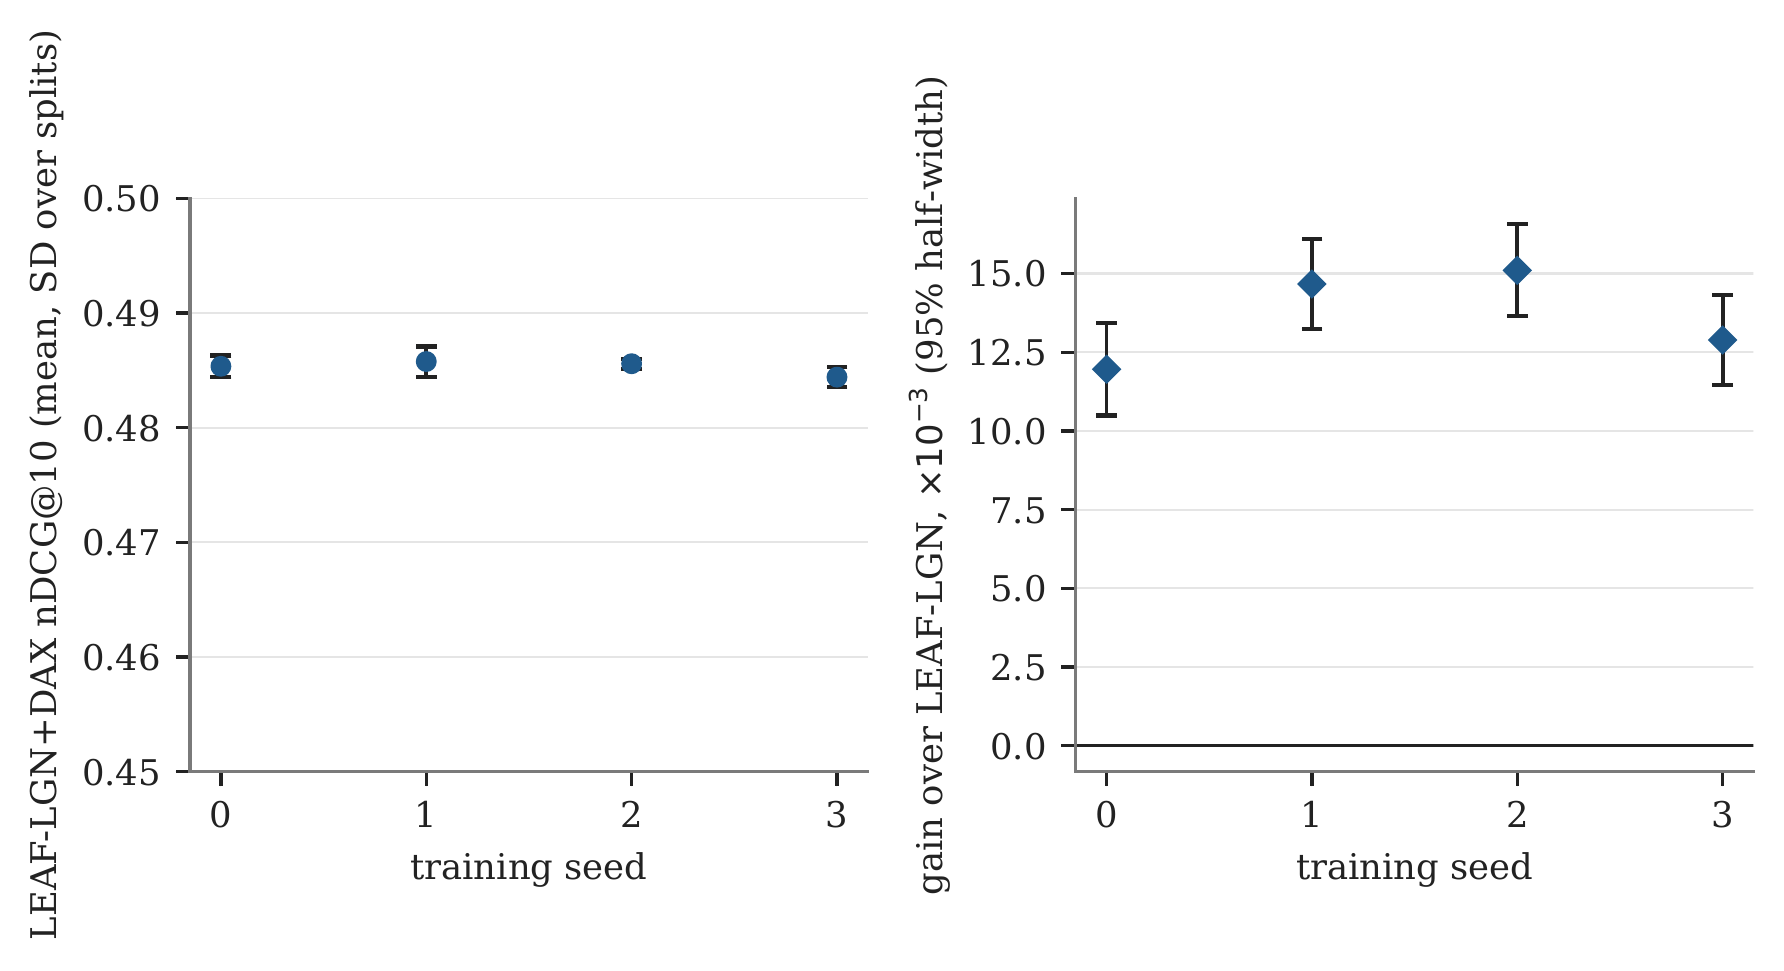
\includegraphics[width=0.85\linewidth]{fig_seeds.png}
\caption{Training seeds 0 to 3 on KuaiRand-27K. Left: LEAF-LGN+DAX mean nDCG@10 with the standard deviation over splits, on an axis from 0.45 to 0.50. Right:
within-seed gain over LEAF-LGN, in units of $10^{-3}$, with the 95\% half-width.}
\label{fig:seeds}
\end{figure}

\section{Counts, baseline values and additional results}
\label{app:counts}

\paragraph{Counts} The KuaiRand-27K data contain 27,077 dataset users. In each split, 8,123 of them form the validation part and 18,954 the test
part. A test user is scored only if a candidate was clicked, which gives 15,809 to 15,913 scored test users per split. Pooled over the five splits,
22,612 distinct users are scored in at least one split. The headroom diagnostic of Section~\ref{sec:res-headroom} uses 22,661 users, all users with
a click in some candidate list. The difference of 49 users consists of users with a click who were in the validation part of all five splits, and
so are never scored.

\paragraph{Baseline values} Table~\ref{tab:methods} gives the mean and standard deviation of each method over the five splits, with the configurations
searched. The means are the means of the split means, as defined in Section~\ref{sec:protocol-stats}.

\begin{table}[tbp]
\centering
\footnotesize
\caption{Methods on KuaiRand-27K (temporal protocol, all users): mean and standard deviation of nDCG@10 over the five splits, and the configurations searched per split.}
\label{tab:methods}
\begin{adjustbox}{max width=\linewidth}
\begin{tabular}{lrrr}
\toprule
Method & Mean & SD & Configurations \\
\midrule
LEAF-LGN+DAX & 0.4854 & 0.0009 & 3,840 \\
LEAF-LGN & 0.4736 & 0.0002 & 12 \\
LEAF-LGN (separate search) & 0.4728 & 0.0011 & 197 \\
PW-LightGCN & 0.4634 & 0.0031 & 20 \\
PW-LightGCN+DAX & 0.4733 & 0.0012 & 3,200 \\
PW-LightGCN, re-trained on its selected configurations & 0.4652 & 0.0017 & 10 \\
r-AdjNorm & 0.4620 & 0.0008 & 8 \\
LightGCN & 0.4576 & 0.0031 & 4 \\
LightGCN+DAX & 0.4709 & 0.0010 & 960 \\
EASE & 0.4507 & 0.0009 & 27 \\
EASE+DAX & 0.4623 & 0.0010 & 8,640 \\
DIN & 0.4675 & 0.0007 & 4 \\
DIN+DAX & 0.4796 & 0.0015 & 1,280 \\
SIM & 0.4590 & 0.0009 & 4 \\
SIM+DAX & 0.4706 & 0.0018 & 1,280 \\
NAVIP & 0.4579 & 0.0020 & 4 \\
IPS-MF & 0.3765 & 0.0008 & 4 \\
DR-JL & 0.3823 & 0.0012 & 4 \\
MRDR & 0.3826 & 0.0008 & 4 \\
\bottomrule
\end{tabular}
\end{adjustbox}
\par\smallskip
\begin{minipage}{\linewidth}\raggedright\footnotesize Mean and SD are taken over the five split means. Configurations searched: backbone trainings times DAX configurations times values of $\gamma$. LEAF-LGN (separate search) is a search of the backbone alone, counted per training and epoch setting, so its count is not in the same unit. PW-LightGCN is, in each split, the best of its three variants on validation. \end{minipage}
\end{table}


\paragraph{KuaiRand-1K} Table~\ref{tab:1k} repeats the primary comparisons on KuaiRand-1K, with 842 test users pooled over the five splits. The
PW-LightGCN with DAX searches 6,400 configurations on this release, against 3,200 at 27K, which favours the baseline. The results are summarised in
Section~\ref{sec:res-1k}.

\begin{table}[tbp]
\centering
\footnotesize
\caption{KuaiRand-1K replication: LEAF-LGN+DAX against the PW-LightGCN with and without DAX (nDCG@10).}
\label{tab:1k}
\begin{adjustbox}{max width=\linewidth}
\begin{tabular}{lrrrcrr}
\toprule
Method or comparison & Mean & SD & Configs & Diff.\ [95\% hw] & NB $p$ & NB $p_{\mathrm{Holm}}$ \\
\midrule
LEAF-LGN+DAX & 0.4590 & 0.0038 & 3,840 &  &  &  \\
PW-LightGCN & 0.4246 & 0.0043 & 20 &  &  &  \\
PW-LightGCN+DAX & 0.4358 & 0.0035 & 6,400 &  &  &  \\
\midrule
LEAF-LGN+DAX minus PW-LightGCN &  &  &  & +37.58 [11.10] & 0.011 & 0.023 \\
LEAF-LGN+DAX minus PW-LightGCN+DAX &  &  &  & +25.82 [9.66] & 0.007 & 0.022 \\
PW-LightGCN+DAX minus PW-LightGCN &  &  &  & +11.76 [8.54] & 0.160 & 0.160 \\
\bottomrule
\end{tabular}
\end{adjustbox}
\par\smallskip
\begin{minipage}{\linewidth}\raggedright\footnotesize Mean: the mean of the five split means. Diff.: the mean over the pooled test users of each user's paired difference (a user's difference is averaged over the splits in which the user is scored). The two are computed over different weightings, so a difference need not equal the difference of the two means shown. For example, the two means shown for LEAF-LGN+DAX and the PW-LightGCN differ by +34.3, against the paired difference of +37.58. KuaiRand-1K: 842 test users pooled over five splits (each split 30\% validation, 70\% test). The users are a subset of the 27K users, so this is a lower-power replication. The PW-LightGCN with DAX searches all 20 PW-LightGCN configurations on this release (6,400 configurations in total), whereas at 27K it searches the 10 selected ones (3,200); this favours the baseline. NB $p_{\mathrm{Holm}}$ is the Holm adjustment over the three comparisons of this table. Split differences ($\times10^{-3}$): LEAF-LGN+DAX minus PW-LightGCN: +36.7 +25.7 +35.6 +37.2 +36.6; LEAF-LGN+DAX minus PW-LightGCN+DAX: +21.3 +20.3 +23.7 +23.1 +27.8; PW-LightGCN+DAX minus PW-LightGCN: +15.4 +5.4 +11.9 +14.1 +8.8.\end{minipage}
\end{table}


\paragraph{Ablation gains} Figure~\ref{fig:ablate} shows the gains of Table~\ref{tab:ablate} with their 95\% half-widths and the five split values.

\begin{figure}[tbp]
\centering
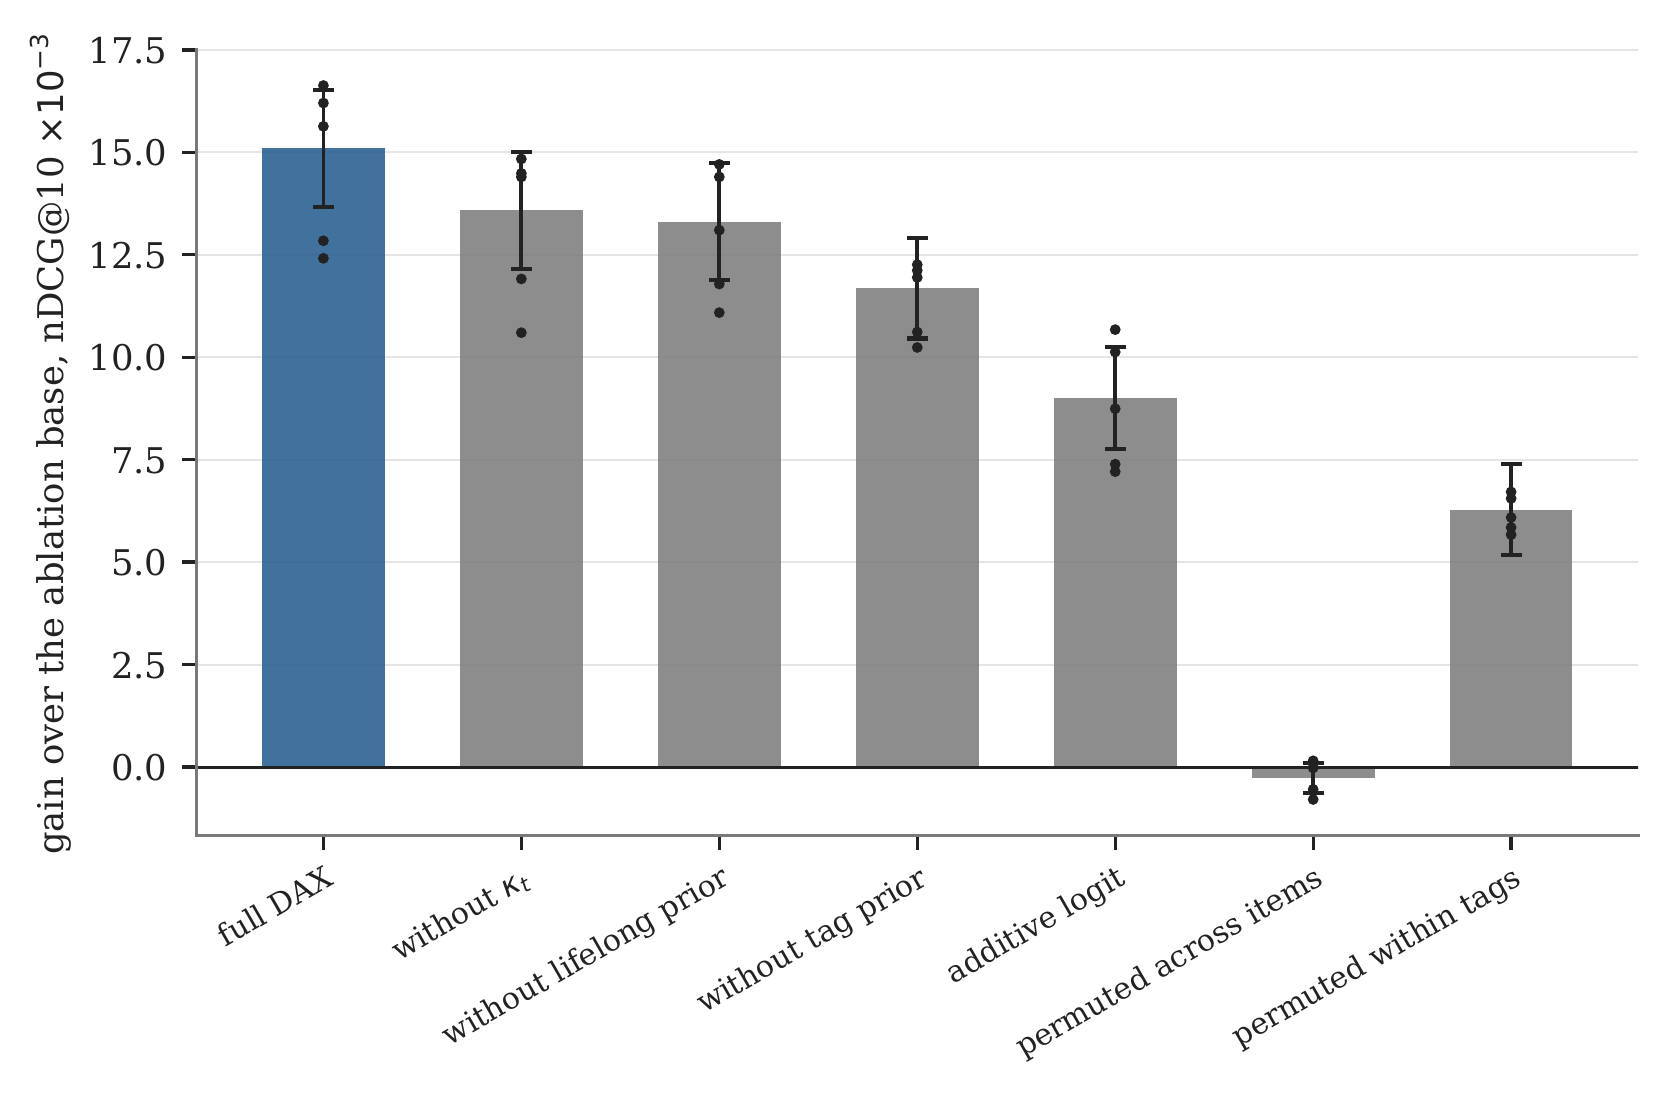
\includegraphics[width=0.8\linewidth]{fig_ablate.png}
\caption{DAX ablations on KuaiRand-27K: gain over the LEAF-LGN base of the ablation search, with the 95\% half-width. Dots are the five splits. The
base is as in Table~\ref{tab:ablate}.}
\label{fig:ablate}
\end{figure}

\paragraph{Closest works} Table~\ref{tab:positioning} collects the works closest to the present one and states the difference from each.

\begin{table}[tbp]
\caption{Closest works and the difference from the present work.}
\label{tab:positioning}
\centering
\footnotesize
\raggedright
\begin{tabular}{p{3.4cm}p{4.2cm}p{5.4cm}}
\toprule
Work & What it estimates, and from which data & Difference from this work \\
\midrule
SIM \citep{pi2020sim}; TWIN \citep{chang2023twin} & CTR from lifelong sequences; policy logs; history and target share item ids & Exposure-conditional statistics; transfer to a disjoint pool through content keys; randomised test; SIM-hard is a baseline, TWIN is not \\
DIN \citep{zhou2018din} & Attention over the last 200 lifelong events; policy logs & Same comparison with DAX added; DIN is a baseline \\
Examination models \citep{richardson2007predicting,craswell2008cascade,chuklin2015clickmodels} & Click as examination times attractiveness; position or list scan & User and scenario examination; no position term; uniform-insertion target \\
Dynamic Bayesian network \citep{chapelle2009dbn} & Perceived versus actual relevance with satisfaction & No satisfaction state \\
Regression-EM \citep{wang2018regressionem,wang2016selection} & Position bias and relevance without randomisation; personal search & Item appeal under a uniform audience; generative fit by EM over user and scenario \\
ExpoMF \citep{liang2016exposure} & Latent exposure fitted by EM & Impressions are observed; latent examination given an impression \\
Unbiased learning to rank \citep{joachims2017unbiased} & Inverse-propensity weighted losses & Generative model instead of a weighted loss \\
Occupancy \citep{mackenzie2002occupancy} & Presence and detection from repeated surveys & Same likelihood structure; no recommender use found \\
Small-area estimation \citep{fay1979smallarea} & Small-area estimates & Used for one centre option of the DAX module \\
NAVIP \citep{kim2022navip} & Propensity-weighted propagation in LightGCN & No lifelong data; no examination model \\
KuaiRand evaluations \citep{gao2022kuairand,zhang2026categorymeans} & Random insertion as the test set & No out-of-pool lifelong history in the test \\
\bottomrule
\end{tabular}
\end{table}

\end{document}
